\documentclass[12pt]{book}

%\usepackage{color}
\usepackage{xcolor}
\usepackage{float}
\usepackage{listings}
\usepackage{array}
\usepackage{geometry}
\usepackage{graphicx}
\usepackage{longtable}
\usepackage{tabu}
\usepackage{cite}
\usepackage{url}
% \usepackage{hyperref}

\title{Discrete-Event Simulation\\
       of Queueing Systems in \texttt{Java}:\\
       The \texttt{jsimulation}
       and
       \texttt{jqueues}
       Libraries\\
       \mbox{ } \\
       Guided Tour}
\author{Jan de Jongh}
\date{Release 5.2\\
	  \mbox{ } \\
	  {\bf DRAFT}\\
	  \mbox{ }
	  \\{\bf Print/Release Date 20180407}}

\lstset
{
  language=Java,
  basicstyle=\ttfamily,
  commentstyle=\textit,
  keywordstyle=\color{red}\bfseries,
  tabsize=2,
  frame=single,
  escapeinside={<@}{@>}
}

\newfloat{lstfloat}{htbp}{lop}
\floatname{lstfloat}{Listing}

\begin{document}

\maketitle

% \chapter*{}
% \begin{center}
% {\em Dedicated to Graham Birtwistle.} \\
% \mbox{ } \\
% {\em In memory of Ole-Johan Dahl and Kristen Nygaard.}
% \end{center}

\chapter*{Preface}
\label{chap:preface}
Personally,
  I (merely) scratched the surface of queueing theory
  at Twente University back in the eighties,
  while working on my Master's Thesis
  on an operating system for {\em transputers}.
Transputers are fast RISC processors
  with multiple on-chip communication links;
  back then, they were envisioned to become the building blocks
  of future massively parallel computer systems.
Since our main applications of interest were in robotics,
  I attempted basic queueing theory in an attempt to find
  hard real-time response-time guarantees,
  in order to meet physical-world, mostly safety-related, deadlines.

During the largest part of the nineties,
  I worked on my PhD at Delft University of Technology.
This time,
  I got to study queueing systems modeling
  {\em distributed computing systems},
  which by then had overtaken parallel systems
  in terms of scientific interest.
The main purpose of the research was to devise
  and analyze scheduling strategies for
  dividing in space and in time
  the computing resources of a
  (closed) distributed system among groups of users,
  according to predefined policies (named
  {\em share scheduling\/} at that time).
In order to gain quantitative insight,
  I used the classic \lstinline|DEMOS|
  (Discrete Event Modeling On Simula) software
  running on the \lstinline|SIMULA|
  programming language.
I made several modifications and extensions to the software,
  in order for it to suit my needs.
For instance,
  it lacked support for so-called
  {\em processor-sharing\/}
  queueing disciplines in which
  a server ("processor") distributes
  at any time its service capacity
  among (a subset of) jobs present.
In addition,
  I needed a non-standard set of statistics
  gathered from the simulation runs.
In the end,
  both \lstinline|DEMOS| and \lstinline|SIMULA| itself
  proved flexible enough to study the research questions.

Like \lstinline|DEMOS|,
  the \lstinline|jsimulation|
  and \lstinline|jqueues|
  \lstinline|Java|
  software packages described in this book
  feature discrete-event simulation
  of queueing systems.
The libraries are, as a combo,
  somewhat comparable to
  the \lstinline|DEMOS|,
  yet there are important differences nonetheless.
For instance, the libraries
  focus exclusively at {\em algorithmic\/}
  modeling of queueing systems and job visits;
  they do not cover additionally required features
  like sophisticated random-number generation,
  probability distributions,
  gathering and analyzing statistics,
  and sophisticated reporting;
  features all integrated in \lstinline|DEMOS|.
In that sense, \lstinline|DEMOS|
  is a more complete package.
On the other hand,
  the packages feature a larger range of
  queueing-system types,
  and, for instance,
  a model for constructing new queueing systems
  through {\em composition\/} of
  other queues.
In addition,
  much care has been put into the
  {\em atomicity\/} of certain events,
  which allows for a wider range of
  {\em queue invariants\/} supported.
Despite these differences,
  \lstinline|DEMOS| has been a major inspiration
  in the design and implementation of
  \lstinline|jsimulation|
  and \lstinline|jqueues|.

For my current employer, TNO,
  I have performed, over the past decade
  (or even decades?),
  many simulation studies in \lstinline|Java|
  related to the vehicle-to-vehicle communications
  in (future) Intelligent Transportation Systems,
  studying, for instance,
  position dissemination over CSMA/CA wireless networks
  for Cooperative Adaptive Cruise Control
  and Platooning.
At some point,
  I realized that it would be feasible to
  extract some useful and stable
  \lstinline|Java| libraries from my ever increasing
  software repositories,
  and release them into the public domain.
So, in a way,
  the libraries can be considered "collateral damage" from a variety of projects.

% I have dedicated the software and this documentation,
%   with gratitude,
%   to the designer of \lstinline|DEMOS|,
%   Graham Birtwistle
%   and, in memory,
%   to the designers of \lstinline|SIMULA|,
%   Ole-Johan Dahl and Kristen Nygaard.

\chapter{Introduction}
\label{chap:intro}
Queueing systems deal with the general notion of {\em waiting\ }
  for (the completion of) "something".
They are ubiquitously and often annoyingly present in our everyday lives.
If there is anything we do most in life,
  it is probably {\em waiting\ } for something to
  happen (finally winning a non-trivial prize in the State Lottery
          after paying monthly tickets over the past thirty years),
  arrive (the breath-taking dress we ordered from that webshop
          against warnings in the seller's reputation blog),
  change (the reception of many severely bad hands in the poker game
          we just happened to ran into),
  stop (the constant flipping into red of traffic lights
        while we are just within breaking distance
        in our urban environment),
  or
  resume (the heater that regularly happens to have
          a mind of its own during
          winter months).

Queueing systems also appear in computer systems and networks,
  in which they schedule available shared resources
  like processors, memory, and network ports
  among clients like
  computing applications.
Or in wireless communications,
  where so-called 'listen-before-talk'
  access protocols (CSMA/CA) as used in wireless Local Area Networks
  monitor the received power level at the input stage
  in order to assess whether the
  transmission medium is idle
  before attempting to transmit.
Or in automated production lines,
  where a partial product is routed to visit
  several service stations in sequence,
  each of them performing a specific task to the
  product.

Perhaps surprisingly given their wide variety in terms of applications,
  queueing systems usually share a common concept:
  a set of objects we will call {\em jobs\/}
  has to visit a set of objects we will call {\em queues},
  in order to get something done.
Depending on the complexity of the task to be performed,
  on the service capacity of the queue,
  and on the available competition among jobs,
  such a visit may vary in length (i.e., in sojourn time).
This perhaps explains the great interest from the mathematical community
  in {\em queueing theory\/}:
  One often needs only a handful of variables and assumptions
    in order to model a wide range of applications.
In most cases,
  the effects of these assumptions
  are modeled with
  suitable stochastic processes.

Despite great results in deriving closed-form analytic expressions
  for many queueing models,
  many more others are mathematically intractable.
In order to gain quantitative insight into these models,
  one often resorts or needs to resort to {\em discrete-event simulation},
  appropriately modeling queue scheduling behavior,
  and subjecting it to a workload consisting of jobs
  with appropriate parameters
  as to the amount of work each job requires,
  and the time between consecutive job arrivals.
Even though discrete-event simulation
  does not provide closed-form solutions,
  they are often very handy and capable of,
  for instance, quantitative comparisons
  between various scheduling strategies.

This document introduces \lstinline|jsimulation|
  and \lstinline|jqueues|,
  open-source \lstinline|java|
  software libraries
  for discrete-event simulation of queueing systems.
Its main purpose is to expose you to the most
  important concepts in the libraries,
  and to get you going with your simulation studies.
By no means is this document complete
  in its description of \lstinline|jsimulation|
  and \lstinline|jqueues|,
  nor is it intended to be,
  and for more detailed information we refer the reader to the
  "JQueues Reference Manual"\footnote{
The JQueues Reference Manual is currently being written,
  and will be available as an e-Book.}
  if you need precise specification
  of the libraries, and to the "JQueues Developer Manual"\footnote{
  	The JQueues Developer Manual is currently being written,
  	and will be available as an e-Book.}
  if you want or need to extend either library
  (e.g., to add your own queueing discipline).

In Section \ref{chap:install} of the present document
  we provide installation (and build) instructions,
  and in Section \ref{chap:hello-world}
  we present our "Hello World" example.
In subsequent sections, in rather random order,
  we provide additional details and examples on
  the use of both libraries;
  attempting to allow linear reading.
However,
  this is a living document
  and sections are added on demand and when time permits.

Any feedback on the clarity and/or correctness of the text
  is highly appreciated.
Please use the {\em Issues\/} section on \lstinline|github| to that purpose\footnote{
  See \texttt{https://github.com/jandejongh/jqueues-guided-tour}.}.

\chapter{Installation}
\label{chap:install}
{\bf Author's Note:} At this time of writing (end of March 2018),
the libraries are {\em not yet\/} available from Maven Central!
{\bf Use Option 1 below!}

\section{The \texttt{jsimulation} and \texttt{jqueues} Libraries}

In order to use \lstinline|jsimulation|
  and \lstinline|jqueues|, you have to install
  them first,
  which requires an Internet connection.
The first public releases of \lstinline|jqueues| and
  \lstinline|jsimulation| have version number \lstinline|5.0.0|;
  they were released under the Apache v2.0 license.
From that version number onward,
  both libraries are distributed as \lstinline|Maven|
  projects
  available from \lstinline|github.com|
  and the Maven Central Repository
  (whichever suits you).
  
Since both \lstinline|jsimulation|
  and \lstinline|jqueues| are libraries
  and hardly support stand-alone operation,
  we assume that you intend to install
  them both as dependencies to your own project.
You have several options, but the two most obvious ones are:
\begin{itemize}
	\item Install the libraries from \lstinline|github|,
	        open them as Maven {\em projects\/} in your IDE
	        and add them as dependencies to your own project.
	      If you use Maven yourself for the latter,
	        you only have to add
	        the dependency on \lstinline|jqueues| in the
	        \lstinline|pom.xml|.
	      (You do not have to add \lstinline|jsimulation|
            because Maven does this automatically for you.)
	\item Create your own Maven project and add
	        \lstinline|jqueues| as a dependency,
	        taken from the Maven Central Repository.
\end{itemize}
In both cases,
  you will need \lstinline|maven| installed and properly configured on your system.
It is also highly recommended to install
  \lstinline|maven| support in your IDE,
  so that it can directly open \lstinline|maven| projects.

In the first case, you need \lstinline|git| as well,
  and you should clone both libraries
  from \lstinline|github| as shown below:
\begin{itemize}
	\item \lstinline|$ git clone https://www.github.com/jandejongh/jsimulation|
	\item \lstinline|$ git clone https://www.github.com/jandejongh/jqueues|
\end{itemize}
Note that \lstinline|jsimulation| and \lstinline|jqueues|
  can only be built against \lstinline|Java 1.8| and higher.

In the second case,
  add the XML fragment shown in Listing \ref{jqueues_pom_dependency}
  to the dependencies
  section in your \lstinline|pom.xml|.
Please make sure that you double-check the version number in the XML file\footnote{
You may want to verify the latest stable release number
from either \lstinline|github| or Maven Central.
This Guided Tour applies to release 5.1.0 and beyond.}. 
\begin{lstfloat}
\begin{lstlisting}[
	caption={The \texttt{dependency} section for \texttt{jqueues} in a \texttt{pom.xml}.},
	label=jqueues_pom_dependency,
	basicstyle=\tiny]
<dependency>
	<groupId>nl.jdj</groupId>
	<artifactId>jqueues</artifactId>
	<version>5.1.0</version>
	<scope>compile</scope>
	<type>jar</type>
</dependency>	
\end{lstlisting}
\end{lstfloat}
The second case is safer as it uses stable, frozen, versions
  of the libraries released to Maven Central.
These releases are signed and cannot be changed without
  increasing the version number.
  
\section{Version Numbering}

For both libraries, we use three-level version numbering:
\begin{itemize}
	\item The third, lowest, level is reserved for bug fixes,
	        \lstinline|javadoc| improvements
	        and code (layout) "beautifications".
	\item The second, middle, level is reserved for functional extensions
	        that do not break existing code (with the same major version number).
	      Think of adding another queue, job or listener type.
	\item The third, major, level is reserved for changes to the core
	        interfaces and classes that are likely to break existing code.
\end{itemize}
This implies that you can (should be able to) always "upgrade" to a later version
  from Maven Central
  as long as the major number remains the same.
Upgrading from \lstinline|github.com| requires a bit of care,
  as the latest version may not be stable yet.
  
Despite the fact that we take utmost efforts
  to {\em not\/} break existing code
  with upgrades of middle and minor version numbers,
  we cannot always avoid this.
For instance,
  we may realize that a method should be
  \lstinline|final| or \lstinline|private|
  and attempt to fix that in an apparent innocent update,
  but you may have overridden (or used)
  that particular method already in your code
  to suit your own purposes.
Needless to say,
  we did not expect you to override (or just use) that particular method in your code,
  just as well as you did not expect that you were not supposed to do so.
But in the end,
  your code may not be compile-able after the upgrade.
In order to avoid this, we recommend that you
\begin{itemize}
  \item Prefer interface methods rather than specific ones from classes,
        since the chance that we consider updates of the interface
        as being "minor" is virtually nil.
  \item Only override methods for which the \lstinline|javadoc| explicitly
        states that they are intended to be overridden.
\end{itemize}

\section{The \texttt{jqueues-guided-tour} Project}

All example code shown in this document is available
  from the \lstinline|jqueues-guided-tour|
  project on \lstinline|github|.
The code is organized as a Maven project.
In addition to the example code,
  it also contains all the source 
  files (\LaTeX\ and other)
  to the present document.
Bear in mind, though, that the documentation and
  example code in \lstinline|jqueues-guided-tour|
  are both released under a more restrictive license than
  \lstinline|jsimulation| and \lstinline|jqueues|.
In short, you are allowed to use the documentation and
  example code to whatever purpose.
You may also redistribute both in unmodified form.
However,
  redistributing {\em modified\/} versions
  of either or both of them
  requires the explicit permission from
  the legal copyright holder.

\chapter{Hello World: FCFS}
\label{chap:hello-world}
In this section,
  we introduce our "Hello World" application for
  \lstinline|jqueues|\footnote{
  	In this Chapter,
  	whenever we refer to \texttt{jqueues},
  	we silently assume that \texttt{jsimulation}
  	is installed as well.},
  consisting of a \lstinline|FCFS| queue
  subject to arrivals of jobs with varying required service times.

In order to perform a simulation study in \lstinline|jqueues|,
  the following actions need to be taken:
\begin{itemize}
\item The creation of an event list;
\item The construction of one or more queues attached to the event list;
\item The selection of the method for listening to the queue(s);
\item The creation of a workload consisting of jobs
        and appropriately scheduling it onto the event list;
\item The execution of the event list;
\item The interpretation of the results,
        typically from the listener output.
\end{itemize}
Without much further ado,
  we show our "Hello World" example
  in Figure \ref{simExample1_main}.
We first create a single event list of type \lstinline|DefaultSimEventList|
  and a \lstinline|FCFS| queue attached to the event list
  (by virtue of the argument of \lstinline|FCFS|'s constructor).
On the queue, we register a newly created
  \lstinline|StdOutSimEntityListener|,
  issuing notifications to the standard output.
Note that queues and jobs are so-called {\em entities\/};
  these are the relevant objects with state subject to event invocation.
Subsequently,
  we create ten jobs named "0", "1", "2", $\ldots$,
  scheduled for arrival at the queue
  at $t=0$, $t=1$, $t=2$, $\ldots$,
  respectively,
  and set their respective service times.
We then schedule each job arrival on the event list.
Finally, we "run" the event list, i.e.,
  let it process the arrivals.

\begin{lstfloat}
\begin{lstlisting}[
  caption={A simple simulation with a single FCFS queue and ten jobs.},
  label=simExample1_main,
  basicstyle=\tiny]

  final SimEventList el = new DefaultSimEventList (0);
  final SimQueue queue = new FCFS (el);
  queue.registerSimEntityListener (new StdOutSimEntityListener ());
  for (int j = 0; j < 10; j++)
  {
    final double jobServiceTime = (double) 2.2 * j;
    final double jobArrivalTime = (double) j;
    final String jobName = Integer.toString (j);
    final SimJob job = new DefaultSimJob (null, jobName, jobServiceTime);
    SimJQEventScheduler.scheduleJobArrival (job, queue, jobArrivalTime);
  }
  el.run ();

\end{lstlisting}
\end{lstfloat}

The event list type
  \lstinline|DefaultSimEventList|
  will suffice for almost all practical cases,
  but it is essential to note already that
  a {\em single\/} event-list instance is typically used
  throughout {\em any\/} simulation program.
Its purpose of the event list is to hold scheduled {\em events\/}
  in non-decreasing order of {\em schedule time},
  and, upon request (in this case through \lstinline|el.run|),
  starts processing the scheduled events in sequence,
  invoking their associated {\em actions}.
In this case,
  the use of events remains hidden,
  because jobs are scheduled through the use of utility method
  \lstinline|scheduleJobArrival|.
The zero argument to the constructor denotes
  the simulation start time.
If you leave it out, the start time defaults to $-\infty$.

Our queue of choice is First-Come First-Served (FCFS).
The constructor takes the event list \lstinline|el|
  as argument.
The queueing system consists of a queue with infinite
  places to hold jobs,
  and a single server that "serves" the jobs in the queue in order
  of their arrival.
Once a queue has finished serving the (single) job,
  the job {\em departs\/} from the system.

So how long does it take to serve a job?
Well, in \lstinline|jqueues|,
  the default behavior is that
  a queue requests the job for its
  {\em required service time}.
In the particular case of \lstinline|DefaultSimJob|
  (there are many more job types),
  we provide a fixed service time (at {\em any\/} queue)
  upon creation through the third argument of the constructor.
  
The first argument of the \lstinline-DefaultSimJob-
  is the event list to which it is to be attached.
For jobs (well, at least the ones derived from \lstinline|DefaultSimJob|),
  it is often safe to set this to \lstinline|null|,
  although we could have equally well set it to \lstinline|el|.
However, {\em queues must always be attached to the event list\/};
  a \lstinline|null| value upon construction will throw an exception.

The (approximate) output of the code fragment
  of Listing \ref{simExample1_main}
  is shown in Listing \ref{simExample1_out} below.
Remarkably,
  the listing only shows two types of notifications,
  viz.,
  \lstinline|UPDATE|
  and
  \lstinline|STATE_CHANGED|,
  the latter of which can hold
  multiple "sub"-notifications.
Each notification outputs
  the name of the listener,
  the time on the event list,
  the queue (entity) that issues the notification,
  the notification's actual "major" type
  (\lstinline|UPDATE| or \lstinline|STATE_CHANGED|)
  and, if present,
  the sub-notifications.

\begin{lstfloat}
\begin{lstlisting}[
  caption={Example output of Listing \ref{simExample1_main}.},
  label=simExample1_out,
  basicstyle=\tiny]

StdOutSimEntityListener t=0.0, entity=FCFS: STATE CHANGED:
  => ARRIVAL [Arr[0]@FCFS]
  => START [Start[0]@FCFS]
  => DEPARTURE [Dep[0]@FCFS]
StdOutSimEntityListener t=1.0, entity=FCFS: UPDATE.
StdOutSimEntityListener t=1.0, entity=FCFS: STATE CHANGED:
  => ARRIVAL [Arr[1]@FCFS]
  => START [Start[1]@FCFS]
  => STA_FALSE [StartArmed[false]@FCFS]
StdOutSimEntityListener t=2.0, entity=FCFS: UPDATE.
StdOutSimEntityListener t=2.0, entity=FCFS: STATE CHANGED:
  => ARRIVAL [Arr[2]@FCFS]
StdOutSimEntityListener t=3.0, entity=FCFS: UPDATE.
StdOutSimEntityListener t=3.0, entity=FCFS: STATE CHANGED:
  => ARRIVAL [Arr[3]@FCFS]
StdOutSimEntityListener t=3.2, entity=FCFS: UPDATE.
StdOutSimEntityListener t=3.2, entity=FCFS: STATE CHANGED:
  => DEPARTURE [Dep[1]@FCFS]
  => START [Start[2]@FCFS]
StdOutSimEntityListener t=4.0, entity=FCFS: UPDATE.
StdOutSimEntityListener t=4.0, entity=FCFS: STATE CHANGED:
  => ARRIVAL [Arr[4]@FCFS]
StdOutSimEntityListener t=5.0, entity=FCFS: UPDATE.
StdOutSimEntityListener t=5.0, entity=FCFS: STATE CHANGED:
  => ARRIVAL [Arr[5]@FCFS]
StdOutSimEntityListener t=6.0, entity=FCFS: UPDATE.
StdOutSimEntityListener t=6.0, entity=FCFS: STATE CHANGED:
  => ARRIVAL [Arr[6]@FCFS]
StdOutSimEntityListener t=7.0, entity=FCFS: UPDATE.
StdOutSimEntityListener t=7.0, entity=FCFS: STATE CHANGED:
  => ARRIVAL [Arr[7]@FCFS]
StdOutSimEntityListener t=7.6000000000000005, entity=FCFS: UPDATE.
StdOutSimEntityListener t=7.6000000000000005, entity=FCFS: STATE CHANGED:
  => DEPARTURE [Dep[2]@FCFS]
  => START [Start[3]@FCFS]
StdOutSimEntityListener t=8.0, entity=FCFS: UPDATE.
StdOutSimEntityListener t=8.0, entity=FCFS: STATE CHANGED:
  => ARRIVAL [Arr[8]@FCFS]
StdOutSimEntityListener t=9.0, entity=FCFS: UPDATE.
StdOutSimEntityListener t=9.0, entity=FCFS: STATE CHANGED:
  => ARRIVAL [Arr[9]@FCFS]
StdOutSimEntityListener t=14.200000000000001, entity=FCFS: UPDATE.
StdOutSimEntityListener t=14.200000000000001, entity=FCFS: STATE CHANGED:
  => DEPARTURE [Dep[3]@FCFS]
  => START [Start[4]@FCFS]
StdOutSimEntityListener t=23.0, entity=FCFS: UPDATE.
StdOutSimEntityListener t=23.0, entity=FCFS: STATE CHANGED:
  => DEPARTURE [Dep[4]@FCFS]
  => START [Start[5]@FCFS]
StdOutSimEntityListener t=34.0, entity=FCFS: UPDATE.
StdOutSimEntityListener t=34.0, entity=FCFS: STATE CHANGED:
  => DEPARTURE [Dep[5]@FCFS]
  => START [Start[6]@FCFS]
StdOutSimEntityListener t=47.2, entity=FCFS: UPDATE.
StdOutSimEntityListener t=47.2, entity=FCFS: STATE CHANGED:
  => DEPARTURE [Dep[6]@FCFS]
  => START [Start[7]@FCFS]
StdOutSimEntityListener t=62.60000000000001, entity=FCFS: UPDATE.
StdOutSimEntityListener t=62.60000000000001, entity=FCFS: STATE CHANGED:
  => DEPARTURE [Dep[7]@FCFS]
  => START [Start[8]@FCFS]
StdOutSimEntityListener t=80.20000000000002, entity=FCFS: UPDATE.
StdOutSimEntityListener t=80.20000000000002, entity=FCFS: STATE CHANGED:
  => DEPARTURE [Dep[8]@FCFS]
  => START [Start[9]@FCFS]
StdOutSimEntityListener t=100.00000000000001, entity=FCFS: UPDATE.
StdOutSimEntityListener t=100.00000000000001, entity=FCFS: STATE CHANGED:
  => DEPARTURE [Dep[9]@FCFS]
  => STA_TRUE [StartArmed[true]@FCFS]

\end{lstlisting}
\end{lstfloat}

Apart from the \lstinline-STATE CHANGED-, \lstinline-UPDATE-
  and \lstinline-START_ARMED- lines in the output,
  the notifications pretty much speak for themselves.
We even get notified when jobs start service (\lstinline-START-).
The \lstinline-START_ARMED- notifications
  refer to state changes in a special \lstinline|boolean| attribute of a
  queue named its \lstinline-StartArmed- property.
Since you will hardly need it in practical applications,
  we will not delve into it,
  but it is crucial for the implementation
  of certain more complex (composite) queueing systems.
Suffice it to say that the \lstinline|StartArmed| property
  {\em in this particular case\/}
  signals whether the queue is idle.

The two top-level notification types,
  \lstinline|UPDATE| and \lstinline|STATE CHANGED|
  are essential.
Upon every change to a queue's state,
  the queue is obliged to issue the fundamental \lstinline|STATE CHANGED| notification,
  exposing the queue's new state (including its notion of time).
The \lstinline|UPDATE| notification
  has the same function,
  but it is fired {\em before\/} any changes have been applied,
  thus revealing the queue's {\em old\/} state,
  including the time at which the old state was obtained.
Hence,
  every \lstinline|STATE CHANGED| notification
  {\em must\/} be preceded with an
  \lstinline|UPDATE| notification.
The \lstinline|UPDATE| notification is
  crucial for the implementation of statistics
  (among others).
  
The use of \lstinline|STATE_CHANGED| notifications may
  appear strange at first sight
  as many other implementations would
  report each of the sub-notifications individually.
However, an important aspect of a queue's contract is that
  {\em it must report state changes atomically
       in order to meet queue invariants}.
This means that listeners,
  when notified,
  will always see the queue in a consistent state,
  i.e., in a state that respects the invariant(s).
This is one of the (we think) most distinguishing features of
  \lstinline|jqueues|.
Going back to our example: An important invariant of FCFS
  and many other queueing systems
  is that there cannot be jobs
  waiting in queue while the server is idle.
It is easy to see that individual notifications for
  \lstinline|ARRIVAL| and \lstinline|START| would
  lead to violations of this invariant:
  Suppose that a job arrives at an idle FCFS queue.
  Using individual notifications,
  the queue has no other option than to
  issue a \lstinline|ARRIVAL|
  notification
  immediately followed by a \lstinline|START|.
In between both, the queue would expose a state
  that is inconsistent with the invariant
  because the server is idle (the job has not started yet),
  while there is a job in its waiting queue.
Note that another invariant of FCFS is that
  it cannot be serving jobs with zero required service time.
This explains the arrival, start and departure sub-notifications
  for job $0$ are all in a single atomic \lstinline|STATE_CHANGED|.
  
This concludes our "Hello World" example.
There is obviously a lot more to tell,
  but the good news is that our example
  has already revealed the most important concepts
  of \lstinline|jqueues| like
  the event list, events, entities, queues, jobs, listeners
  and notifications.
The remaining complexity is in the richness and variation of these
  basic concepts.

%\chapter{Events, Actions and the Event List}
%\label{chap:events-actions-event-list}
%This chapter describes the event and event-list features
  that are available from the \lstinline{jsimulation} package.
Note that \lstinline{jsimulation} is a dependency of \lstinline{jqueues}.

\section{Creating the Event List and Events}

At the very heart of every simulation experiment
  in \lstinline{jqueues}
  is the so-called {\em event list}.
The event list obviously holds the events,
  keeps them ordered,
  and maintains a notion of "where we are" in a simulation run.
Together, an event list and the events it contains define
  the precise sequence of actions taken in a simulation.
The following code snipplet shows how to create an event list and
  schedule two (empty) events, one at $t_{1}=5.0$ and one at $t_{2}=10$,
  and print the resulting event list on \lstinline{System.out}:
\begin{lstlisting}
final SimEventList el = new DefaultSimEventList ();
final SimEvent e1 = new DefaultSimEvent (5.0);
final SimEvent e2 = new DefaultSimEvent (10.0);
el.add (e1);
el.add (e2);
el.print ();
\end{lstlisting}
In \lstinline{jsimulation},
  the event list is of type \lstinline{SimEventList};
  events are of type \lstinline{SimEvent},
  respectively.
Since both of them are Java {\em interfaces}, you need implementing classes
  to instantiate them: \lstinline{DefaultSimEventList} for an event list;
  \lstinline{DefaulSimEvent} for an event.
Typically,
  you instantiate a single event list for a simulation experiment,
  and numerous events.

The \lstinline{double} argument in the \lstinline{DefaultSimEvent} constructor
  (of which there are several)
  is the {\em schedule time\/} of the event on the event list.
Perhaps surprisingly,
  in \lstinline{jsimulation},
  the schedule time is actually held on the event,
 {\em not\/} on the event list.
Also, a \lstinline{SimEventList} is inheriting from \lstinline{SortedSet}
  from the Java Collections Framework.
These choices have the following consequences:
\begin{itemize}
  \item Each \lstinline{SimEvent} can be present {\em at most once\/} in a \lstinline{SimEventList}.
        You cannot reuse a single event instance (like a job creation and arrival event)
          by scheduling it multiple times on the event list.
        Instead, you must either use separate event instances, or reschedule the event
          the moment it leaves the event list.
  \item You cannot (more precisely, {\em should not\/}) modify the time on the event while it is
          scheduled on an event list.
  \item You always have access to the (intended) schedule time of the event, without having to
          refer to an event list (if the event is scheduled at all) or use a separate
          variable to keep and maintain that time.
  \item The events must be equipped with a {\em total ordering\/} (imposed by \lstinline{SortedSet})
          and distinct events should not be equal (imposed by us).
          This means that for each pair of (distinct) events scheduled on a \lstinline{SimEventList},
          one of them is always strictly larger than the other
          (in the ordering, they cannot be "equal").
\end{itemize}

The output of the code snipplet is something like\footnote{
We may have improved the layout in the meantime.}:
\begin{lstlisting}[basicstyle=\tiny]
SimEventList {X}.DefaultSimEventList@{Y}, class=DefaultSimEventList, time=-Infinity:
  t=5.0, name=No Name, object=null, action=null.
  t=10.0, name=No Name, object=null, action=null.
\end{lstlisting}
The output shows the name of the event list (as obtained from its \lstinline{toString} method)
  and the current time ($-\infty$) in the first row, and then the events in the list
  in the proper order.
By the way, we modified the output; the markers \lstinline|{X}| and \lstinline|{Y}|
  represents strings that most likely deviate on your system.

The output also shows the four properties of an event: its time, name, user object, and action.
These will be described in more detail in the next section.

\section{Event Properties and Event Constructors}

A \lstinline{SimEvent} has the following properties:
\begin{itemize}
\item Time:   The (intended) schedule time of the event (default $-\infty$).
\item Name:   The name of the event, which is only used for logging and output (default "No Name").
\item Object: A general-purpose object available for storing information associated with the event
              (\lstinline{jsimulation} nor \lstinline{jqueues} uses this field; its
              default value is \lstinline{null}).
\item Action: The action to take, a \lstinline{SimEventAction} (default \lstinline{null}),
                described in the next section.
\end{itemize}
Each property has corresponding getter and setter methods:

\begin{tabular}{|l|}
  \hline
  {\bf Properties of \lstinline|SimEvent|} \\
  \hline
  \lstinline[basicstyle=\footnotesize]!double getTime ()! \\
  \lstinline[basicstyle=\footnotesize]!void setTime (double)! \\
  \hline
  \lstinline[basicstyle=\footnotesize]!String getName ()! \\
  \lstinline[basicstyle=\footnotesize]!void setName (String)! \\
  \hline
  \lstinline[basicstyle=\footnotesize]!T getObject ()! \\
  \lstinline[basicstyle=\footnotesize]!void setObject (T)! \\
  \hline
  \lstinline[basicstyle=\footnotesize]!SimEventAction getEventAction ()! \\
  \lstinline[basicstyle=\footnotesize]!void setEventAction (SimEventAction)! \\
  \hline
\end{tabular}

Note that \lstinline{T} refers to the so-called {\em generic-type argument\/}
  of \lstinline{SimEvent} (and also of \lstinline|DefaultSimEvent|).
The prototype is \lstinline|SimEvent<T>|, so \lstinline|T| can be any object type.
The use of generic types is explained in some more details in the "Advanced Topics" section,
  but for now \lstinline!T! can be simply read as a \lstinline{Object}.

The next section describes the actions in more detail, but we first provide a list
  of constructors for \lstinline{DefaultSimEvent}:

\begin{tabular}{|l|}
  \hline
  {\bf Constructors of \lstinline|DefaultSimEvent|} \\
  \hline
  \lstinline[basicstyle=\footnotesize]!DefaultSimEvent (String, double, T, SimEventAction)! \\
  \lstinline[basicstyle=\footnotesize]!DefaultSimEvent (double, T, SimEventAction)! \\
  \lstinline[basicstyle=\footnotesize]!DefaultSimEvent (double, SimEventAction)! \\
  \lstinline[basicstyle=\footnotesize]!DefaultSimEvent (double)! \\
  \lstinline[basicstyle=\footnotesize]!DefaultSimEvent ()! \\
  \hline
\end{tabular}

Any non-listed property in a constructor will obtain its default value.

\section{Actions}

A \lstinline{SimEventAction} defined what needs to be done by the time an event
  is {\em executed\/} or {\em processed}.
In Java terms, a \lstinline{SimEventAction} is an interface with
  a single abstract method which is invoked when the event is processed.
Below we show the declaration of the interface:
\begin{lstlisting}[basicstyle=\tiny]
@FunctionalInterface
public interface SimEventAction<T>
{

  /** Invokes the action for supplied {@link SimEvent}.
   *
   * @param event The event.
   *
   * @throws IllegalArgumentException If <code>event</code> is <code>null</code>.
   * 
   */
  public void action (SimEvent<T> event);

}
\end{lstlisting}

There are several ways to create actions for events.
The first and most often used way in our own code is to use anonymous inner classes:
\begin{lstlisting}[basicstyle=\tiny]
final SimEventList el = new DefaultSimEventList ();
final SimEvent e =
  new DefaultSimEvent ("My First Real Event", 5.0, null, new SimEventAction ()
  {
    @Override
    public final void action (final SimEvent event)
    {
      System.out.println ("Event=" + event + ", time=" + event.getTime () + ".");
    }
    @Override
    public String toString ()
    {
      return "My First Action";
    }
  });
el.add (e);
el.print ();
el.run ();
el.print ();
\end{lstlisting}
Note that we are now using the full \lstinline{DefaultSimEvent} constructor,
  passing a name, and supplying a \lstinline{SimEventAction}
  as an anonymous inner class.
In the inner class, we define the \lstinline{action} method,
  and in the meantime override the \lstinline{toString} method
  (to be honest, this was merely to keep the generated text within bounds).
The generated output is:
\begin{lstlisting}[basicstyle=\tiny]
SimEventList {X}.DefaultSimEventList@{Y}, class=DefaultSimEventList, time=-Infinity:
  t=5.0, name=My First Real Event, object=null, action=My First Action.
Event=My First Real Event, time=5.0.
SimEventList {X}.DefaultSimEventList@{Y}, class=DefaultSimEventList, time=5.0:
  EMPTY!
\end{lstlisting}
Clearly, as expected!
However, rote that after "running" the event list, it turns out to be empty,
  and its time is now $t=5.0$, the schedule time of our event.
This is as intended, and will be explained in the next section.
But first we look at an alternative way of attaching
  actions to events:
\begin{lstlisting}[basicstyle=\tiny]
final SimEventList el = new DefaultSimEventList ()
{
  @Override
  public final String toString ()
  {
    return "My Renamed Event List";
  } 
};
final SimEventAction action = new SimEventAction ()
{
  @Override
  public final void action (final SimEvent event)
  {
      System.out.println ("Event=" + event + ", time=" + event.getTime () + ".");
  }
  @Override
  public final String toString ()
  {
    return "A Shared Action";
  }
};
for (int i = 1; i <= 10; i++)
{
  final SimEvent e = new DefaultSimEvent ("Our Event", (double) i, null, action);
  el.add (e);
}
el.print ();
el.run ();
el.print ();
\end{lstlisting}
In this example, we created a single action object
  (again using an anonymous inner class),
  and reuse it among ten distinct events we schedule
  (we cannot reuse those).
We also took the opportunity give our
  event list a friendlier name by overriding its \lstinline{toString} method.
The output is as follows:
\begin{lstlisting}[basicstyle=\tiny]
SimEventList My Renamed Event List, class=, time=-Infinity:
  t=1.0, name=Our Event, object=null, action=A Shared Action.
  t=2.0, name=Our Event, object=null, action=A Shared Action.
  t=3.0, name=Our Event, object=null, action=A Shared Action.
  t=4.0, name=Our Event, object=null, action=A Shared Action.
  t=5.0, name=Our Event, object=null, action=A Shared Action.
  t=6.0, name=Our Event, object=null, action=A Shared Action.
  t=7.0, name=Our Event, object=null, action=A Shared Action.
  t=8.0, name=Our Event, object=null, action=A Shared Action.
  t=9.0, name=Our Event, object=null, action=A Shared Action.
  t=10.0, name=Our Event, object=null, action=A Shared Action.
Event=Our Event, time=1.0.
Event=Our Event, time=2.0.
Event=Our Event, time=3.0.
Event=Our Event, time=4.0.
Event=Our Event, time=5.0.
Event=Our Event, time=6.0.
Event=Our Event, time=7.0.
Event=Our Event, time=8.0.
Event=Our Event, time=9.0.
Event=Our Event, time=10.0.
SimEventList My Renamed Event List, class=, time=10.0:
  EMPTY!
\end{lstlisting}
Again note that the time on the event list after running it
  is the time of the last event we scheduled on it.
In the output, funny enough, the \lstinline{class} of the event list
  is now reported as empty.
This is because we used an anonymous class to construct it!

So, there are different ways of attaching a \lstinline{SimEventAction}
  to a \lstinline{DefaultSimEvent}.
The abundant use of anonymous inner classes as shown here
  is certainly not to everyone's taste,
  but it results in relatively compact code
  (even more through the use of lambda expressions, see {\bf XXX}).

\section{Processing the Event List}

Once the events of your liking are scheduled on the event list,
  you can start the simulation by {\em processing\/} or {\em running\/}
  the event lists.
Processing the event list will cause the event list to
  equentially invoke the actions attached to the events
  in increasing-time order.
There are several ways to process a \lstinline{SimEventList}:
\begin{itemize}
  \item You can process the event list until it is empty with the \lstinline{run} method.
  \item You can process the event list until some specified (simulation) time with the
          \lstinline{runUtil} method.
  \item You can {\em single-step\/} through the event list with the
          \lstinline{runSingleStep} method.
\end{itemize}
You can check whether an event list is being processed through its \lstinline{isRunning}
  method.

While processing, the event list maintains a {\em clock}
  holding the (simulation) time of the current event.
You can get the time from the event list through \lstinline{getTime} nethod,
  although you can obtain it more easily from the event itself.
You can insert new events while it is being processed,
  {\em but these events must not be in the past}.
Once the event list detects insertion of events in the past,
  it will throw and exception.

Note that processing the event list
  is thread-safe in the sense that all methods involved
  need to obtain a {\em lock} before being able to process the list.
Trying to process an event list that is already being processed
  from another thread,
  or from the thread that currently processes the list,
  will lead to an exception.
Note that currently there is no safe, atomic, way
  to process an event list on the condition that is
  is not being processed already.
Though you can check with \lstinline{isRunning}
  whether the list is being processed or not,
  the answer from this method has zero validity lifetime.

The example below shows how to schedule new events
  from event actions; it also shows what happens if you schedule
  events in the past.
\begin{lstlisting}[basicstyle=\tiny]
final SimEventList el = new DefaultSimEventList ()
{
  @Override
  public final String toString ()
  {
    return "The Event List";
  } 
};

final SimEventAction schedulingAction = new SimEventAction ()
{
  private int counter = 0;
  @Override
  public final void action (final SimEvent event)
  {
      System.out.println ("Event=" + event + ", time=" + event.getTime () + ".");
      counter++;
      if (counter < 10)
        // Schedule 1 second from now.
        // Use utility method on SimEventList.
        el.schedule (event.getTime () + 1, this);
      else if (counter == 10)
      {
        // Schedule now.
        el.schedule (event.getTime (), this);
        System.out.println ("Scheduled event now.");
      }
      else
      {
        // Schedule 1 second in the past -> throws exception.
        el.schedule (event.getTime () - 1, this);
        // Never reached.
        System.out.println ("Scheduled event in the past.");
      }
  }
  @Override
  public final String toString ()
  {
    return "Scheduling Action";
  }
};
    
el.schedule (0, schedulingAction);
el.print ();
el.run ();
el.print ();
\end{lstlisting}
The code begins to look familiar.
First, we create the event list, then a single action.
The action is a bit more complicated than before;
  it has an internal \lstinline{counter} in the anynoumous class.
Using the counter, it reschedules itself ten times,
  the first nine times one second in the future,
  the tenth time at exactly the same time.
As mentioned before, this is perfectly legal
  (and, in fact, often used in our own code).
The final attempt to reschedule the action results in an
  exception, because the event is scheduled in the past.
Note that the example also showcases a utility method
  in \lstinline{SimEventList}, viz., \lstinline{schedule (double, SimEventAction)},
  which directly schedules the action on the event list at given time,
  creating a new \lstinline{SimEvent} on the fly.
In a later section we will look in more detail at more utility methods
  on event lists.

The output of the example is shown below\footnote{
  For improved reading, we have left out the full stack-trace of the exception,
  and rearranged the mixed outputs from \lstinline{System.out} and \lstinline{System.err}.
  We will do that without notice in the sequel.
}.
\begin{lstlisting}[basicstyle=\tiny]
SimEventList The Event List, class=, time=-Infinity:
  t=0.0, name=No Name, object=null, action=Scheduling Action.
Event=No Name, time=0.0.
Event=No Name, time=1.0.
Event=No Name, time=2.0.
Event=No Name, time=3.0.
Event=No Name, time=4.0.
Event=No Name, time=5.0.
Event=No Name, time=6.0.
Event=No Name, time=7.0.
Event=No Name, time=8.0.
Event=No Name, time=9.0.
Scheduled event now.
Event=No Name, time=9.0.
Exception in thread "main" java.lang.IllegalArgumentException:
Schedule time is in the past: 8.0 < 9.0!
\end{lstlisting}
Note that in this particular case,
  the exception thrown actually comes with an
  instructive message as to what caused it
  (you tried to schedule something on the event list at $t=8.0$,
   whereas the current time is beyond that, $t=9.0$).
However, in all honesty,
  such messages are not present
  for the majority of exceptions thrown
  as a result of incorrect arguments from user code.
We are currently working on improving this.

The output also shows the expected result from the first \lstinline{el.print} statement:
Only a single event is scheduled!
The others are created and scheduled while the event list is being processed.
It is important to realize that the contents of a \lstinline{SimEventList}
  can always change, as long as these are changes {\em now or in the future}.
By the way, the second invocation of \lstinline{el.print} does not stand a chance;
  it is unreachable because of the exception thrown in \lstinline{el.run}.

\section{Utility Methods for Scheduling Events}

A \lstinline{SimEventList} supports various methods for
  directly scheduling events and actions
  without the need to generate both
  the \lstinline{SimEvent} {\em and\/} the \lstinline{SimEventAction}.
In most cases, the availability of one of the object suffices.
Below we show the most common utility methods for scheduling on a \lstinline{SimEventList}.

\begin{tabular}{|l|}
  \hline
  {\bf Utility methods for scheduling} \\
  \hline
  \lstinline[basicstyle=\footnotesize]!void schedule (E)! \\
    Schedules the event at its own time.\\
  \hline
  \lstinline[basicstyle=\footnotesize]!void schedule (double, E)! \\
    Schedules the event at given time.\\
  \hline
  \lstinline[basicstyle=\footnotesize]!reschedule (double, E)! \\
    Reschedules (if present, else schedules) the event at given new time.\\
  \hline
  \lstinline[basicstyle=\footnotesize]!E schedule (double, SimEventAction, String)! \\
    Schedules the action at given time with given event name.\\
  \hline
  \lstinline[basicstyle=\footnotesize]!void scheduleNow (E)! \\
    Schedules the event now.\\
  \hline
  \lstinline[basicstyle=\footnotesize]!E schedule (double, SimEventAction)! \\
    Schedules the action at given time with default event name.\\
  \hline
  \lstinline[basicstyle=\footnotesize]!E scheduleNow (SimEventAction, String)! \\
    Schedules the action now with given event name.\\
  \hline
  \lstinline[basicstyle=\footnotesize]!E scheduleNow (SimEventAction)! \\
    Schedules the action now with default event name.\\
  \hline
\end{tabular}

Note that \lstinline{E} refers to the so-called {\em generic-type argument\/}
  of \lstinline{SimEventList}.
The prototype is \lstinline!SimEventList<E extends SimEvent>!.
The use of generic types is explained in some more details in the "Advanced Topics" section,
  but for now \lstinline!E! can be simply read as a \lstinline{SimEvent}.

For any of the utilty methods that take a \lstinline{SimEventAction}
  as argument, a new \lstinline{SimEvent} is created on the fly,
  and returned from the method.
Upon return from these methods,
  the newly created event has already been scheduled,
  and you {\em really\/} should not schedule it again.

You may wonder how to {\em remove\/} events and actions from the event list.
Well, since \lstinline{SimEventList} implements the \lstinline{Set} interface for
  \lstinline{SimEvent} members, removing an event \lstinline{e}
  from an event list \lstinline{el} is as simple as
  \lstinline{el.remove (e)}.
Currently, there is no support to remove an action from an event list.
Because actions can be reused, it would require iterating over
  all scheduled events,
  and remove all events with the given action.
It is not hard to implement at all, we just did not do it\footnote{
This code fragment has not been tested.}:
\begin{lstlisting}[basicstyle=\tiny]
public static void removeAction
(final SimEventList eventList, final SimAction action)
{
  if (eventList != null)
  {
    final Iterator it = eventList.iterator;
    while (it.hasNext ())
      if (it.next ().getEventAction () == action)
        it.remove ();
  }
}
\end{lstlisting}
The code fragment silently assumes
  the absence of \lstinline{null} events
  in the event list,
  which is indeed guaranteed,
  and works perfectly for \lstinline{null} actions.
Note the somewhat unexpected method name on \lstinline{SimEvent}
  to get its action, viz., \lstinline{getEventAction}.
This name was chosen in order to avoid potential name clashes.
At the risk of sounding pedantic,
  the explicit use of the iterator
  looks old-fashioned,
  yet allows for
  the safe removal of elements
  from a collection in a loop
  (contrary to a much fancier \lstinline{for} construction).

We conclude with an overview of
  non-scheduling related utility methods
  of \lstinline{SimEventList}:

\begin{tabular}{|l|l|}
  \hline
  {\bf Method} & {\bf Description} \\
  \hline
  \lstinline[basicstyle=\footnotesize]!void print ()! & Prints the event list to \lstinline!System.out!. \\
  \lstinline[basicstyle=\footnotesize]!void print (PrintStream)! & Prints the event list to the stream. \\
  \hline
\end{tabular}

\section{Simultaneous Events}
\label{sec:guided:simultaneous-events}

So far, all events scheduled in our examples had a unique schedule time.
But what if two events have identical schedule times?
The short answer is: The \lstinline|DefaultSimEventList| will
process them {\em in random order}.
Why not respect "insertion order"?
Well, the answers to this seemingly innocent question
are quite involved, and are given in
Section \ref{sec:events-eventlists-actions:simultaneous-events}.

By slightly modifying our first example in Listing \ref{simExample1_main},
we can easily force the occurence of simultaneous events.
In Listing \ref{simExample1_simul_main},
apart from creating and scheduling fewer jobs,
we have reduced the required service time to $1.0$,
and it is trivial to see that for this particular
schedule, the departure of job $1$ coincides
with the arrival of job $2$,
and similarly for jobs $2$ and $3$.
In the output shown in Listing \ref{simExample1_simul_out},
we indeed see that $t=2$,
job $2$ arrives {\em before\/}
the departure of job $1$,
however,
at $t=3$,
job $3$ arrives {\em after\/}
the departure of job $2$.
At both instants in time,
the relative order of the event is,
as mentioned earlied,
completely coincidental.

\begin{lstfloat}
	\begin{lstlisting}[
	caption={An example simulation program with simultaneous events.},
	label=simExample1_simul_main,
	basicstyle=\tiny]
	
	final SimEventList el = new DefaultSimEventList ();
	final int bufferSize = 2;
	final FCFS_B queue = new FCFS_B (el, bufferSize);
	final SimQueueListener listener = new StdOutSimQueueListener ();
	queue.registerSimEntityListener (listener);
	for (int j = 1; j <= 3; j++)
	{
	final double jobServiceTime = 1.0;
	final double jobArrivalTime = (double) j;
	final String jobName = Integer.toString (j);
	final SimJob job = new DefaultSimJob (null, jobName, jobServiceTime);
	SimJQEventScheduler.scheduleJobArrival (job, queue, jobArrivalTime);
	}
	el.run ();
	
	\end{lstlisting}
\end{lstfloat}

\begin{lstfloat}
	\begin{lstlisting}[
	caption={Example output of Listing \ref{simExample1_simul_main}.},
	label=simExample1_simul_out,
	basicstyle=\tiny]
	
	StdOutSimQueueListener t=1.0, entity=FCFS_B[2]: UPDATE.
	StdOutSimQueueListener t=1.0, entity=FCFS_B[2]: STATE CHANGED:
	=> ARRIVAL [Arr[1]@FCFS_B[2]]
	=> START [Start[1]@FCFS_B[2]]
	=> STA_FALSE [StartArmed[false]@FCFS_B[2]]
	StdOutSimQueueListener t=1.0, queue=FCFS_B[2]: ARRIVAL of job 1.
	StdOutSimQueueListener t=1.0, queue=FCFS_B[2]: START of job 1.
	StdOutSimQueueListener t=1.0, queue=FCFS_B[2]: START_ARMED -> false.
	StdOutSimQueueListener t=2.0, entity=FCFS_B[2]: UPDATE.
	StdOutSimQueueListener t=2.0, entity=FCFS_B[2]: STATE CHANGED:
	=> ARRIVAL [Arr[2]@FCFS_B[2]]
	StdOutSimQueueListener t=2.0, queue=FCFS_B[2]: ARRIVAL of job 2.
	StdOutSimQueueListener t=2.0, entity=FCFS_B[2]: STATE CHANGED:
	=> DEPARTURE [Dep[1]@FCFS_B[2]]
	=> START [Start[2]@FCFS_B[2]]
	StdOutSimQueueListener t=2.0, queue=FCFS_B[2]: DEPARTURE of job 1.
	StdOutSimQueueListener t=2.0, queue=FCFS_B[2]: START of job 2.
	StdOutSimQueueListener t=3.0, entity=FCFS_B[2]: UPDATE.
	StdOutSimQueueListener t=3.0, entity=FCFS_B[2]: STATE CHANGED:
	=> DEPARTURE [Dep[2]@FCFS_B[2]]
	=> STA_TRUE [StartArmed[true]@FCFS_B[2]]
	StdOutSimQueueListener t=3.0, queue=FCFS_B[2]: DEPARTURE of job 2.
	StdOutSimQueueListener t=3.0, queue=FCFS_B[2]: START_ARMED -> true.
	StdOutSimQueueListener t=3.0, entity=FCFS_B[2]: STATE CHANGED:
	=> ARRIVAL [Arr[3]@FCFS_B[2]]
	=> START [Start[3]@FCFS_B[2]]
	=> STA_FALSE [StartArmed[false]@FCFS_B[2]]
	StdOutSimQueueListener t=3.0, queue=FCFS_B[2]: ARRIVAL of job 3.
	StdOutSimQueueListener t=3.0, queue=FCFS_B[2]: START of job 3.
	StdOutSimQueueListener t=3.0, queue=FCFS_B[2]: START_ARMED -> false.
	StdOutSimQueueListener t=4.0, entity=FCFS_B[2]: UPDATE.
	StdOutSimQueueListener t=4.0, entity=FCFS_B[2]: STATE CHANGED:
	=> DEPARTURE [Dep[3]@FCFS_B[2]]
	=> STA_TRUE [StartArmed[true]@FCFS_B[2]]
	StdOutSimQueueListener t=4.0, queue=FCFS_B[2]: DEPARTURE of job 3.
	StdOutSimQueueListener t=4.0, queue=FCFS_B[2]: START_ARMED -> true.
	
	\end{lstlisting}
\end{lstfloat}

\section{Infinite Time}
\label{sec:infinite-time}

In the previous section we showed that
events can be scheduled simultaneously.
Another noteworthy feature of a \lstinline|SimEventList|
is that you can schedule events
at $t=-\infty$ and at $t=+\infty$\footnote{
	In honor of Georg Cantor.},
corresponding to the \lstinline|Java|'s
\lstinline|Double.NEGATIVE_INFINITY| and
\lstinline|Double.POSITIVE_INFINITY|,
respectively.
There are, however, some caveats:
\begin{itemize}
	\item All events scheduled at $t=-\infty$ ($t=+\infty$)
	are treated as simultaneous events.
	\item Even though most \lstinline|SimQueue|
	implementations have documented support
	for events at infinity,
	they often behave differently.
	For instance, if a job requires
	a finite amount of service,
	it will most likely depart immediately
	(informally: "$x + \infty = \infty$ for real $x$").
\end{itemize}
In short, caution is advised when scheduling events at infinity.

In our next example shown in Listing \ref{simExample1_infty_main},
with corresponding output in Listing \ref{simExample1_infty_out},
we show how to schedule events at $-\infty$.
We increase to buffer size of the \lstinline|FCFS_B| queue to four
because we do not want to run into job drops in this example.

\begin{lstfloat}
	\begin{lstlisting}[
	caption={An example simulation program with events at $t=-\infty$ and $t=\infty$.},
	label=simExample1_infty_main,
	basicstyle=\tiny]
	
	final SimEventList el = new DefaultSimEventList ();
	final int bufferSize = 4;
	final FCFS_B queue = new FCFS_B (el, bufferSize);
	final SimQueueListener listener = new StdOutSimQueueListener ();
	queue.registerSimEntityListener (listener);
	for (int j = 1; j <= 2; j++)
	{
	final double jobServiceTime = Double.POSITIVE_INFINITY;
	final double jobArrivalTime = Double.NEGATIVE_INFINITY;
	final String jobName = Integer.toString (j);
	final SimJob job = new DefaultSimJob (null, jobName, jobServiceTime);
	SimJQEventScheduler.scheduleJobArrival (job, queue, jobArrivalTime);
	}
	final SimJob job3 = new DefaultSimJob (null, "3", Double.POSITIVE_INFINITY);
	SimJQEventScheduler.scheduleJobArrival (job3, queue, 0.0);
	final SimJob job4 = new DefaultSimJob (null, "4", Double.POSITIVE_INFINITY);
	SimJQEventScheduler.scheduleJobArrival (job4, queue, Double.POSITIVE_INFINITY);
	el.run ();
	
	\end{lstlisting}
\end{lstfloat}

In the example, we schedule two jobs, "1" and "2" at $t=-\infty$.
This is only allowed because the \lstinline|DefaultSimEventList|
initialized itself at $t=-\infty$
(you are not allowed to schedule events "in the past"!).
The jobs have unity required service time,
but as the output shows, this really is irrelevant:
Both jobs arrive (in order of scheduling, but that is a mere coincidence!),
are taken into service, and depart immediately,
all at the moment ($-\infty$) of arrival,
because the required service time is finite.
We also schedule a third job at $t=0$ yet with infinite
required service time,
which is allowed for many queue types.
However, this job never leaves, not even at $t=+\infty$;
it is {\em sticky\/}.
The same goes for job $4$,
also requiring infinite service time,
yet arriving at $t=+\infty$

\begin{lstfloat}
	\begin{lstlisting}[
	caption={Example output of Listing \ref{simExample1_infty_main}.},
	label=simExample1_infty_out,
	basicstyle=\tiny]
	
	StdOutSimQueueListener t=-Infinity, entity=FCFS_B[4]: UPDATE.
	StdOutSimQueueListener t=-Infinity, entity=FCFS_B[4]: STATE CHANGED:
	=> ARRIVAL [Arr[1]@FCFS_B[4]]
	=> START [Start[1]@FCFS_B[4]]
	=> STA_FALSE [StartArmed[false]@FCFS_B[4]]
	StdOutSimQueueListener t=-Infinity, queue=FCFS_B[4]: ARRIVAL of job 1.
	StdOutSimQueueListener t=-Infinity, queue=FCFS_B[4]: START of job 1.
	StdOutSimQueueListener t=-Infinity, queue=FCFS_B[4]: START_ARMED -> false.
	StdOutSimQueueListener t=-Infinity, entity=FCFS_B[4]: UPDATE.
	StdOutSimQueueListener t=-Infinity, entity=FCFS_B[4]: STATE CHANGED:
	=> ARRIVAL [Arr[2]@FCFS_B[4]]
	StdOutSimQueueListener t=-Infinity, queue=FCFS_B[4]: ARRIVAL of job 2.
	StdOutSimQueueListener t=0.0, entity=FCFS_B[4]: UPDATE.
	StdOutSimQueueListener t=0.0, entity=FCFS_B[4]: STATE CHANGED:
	=> ARRIVAL [Arr[3]@FCFS_B[4]]
	StdOutSimQueueListener t=0.0, queue=FCFS_B[4]: ARRIVAL of job 3.
	StdOutSimQueueListener t=Infinity, entity=FCFS_B[4]: UPDATE.
	StdOutSimQueueListener t=Infinity, entity=FCFS_B[4]: STATE CHANGED:
	=> ARRIVAL [Arr[4]@FCFS_B[4]]
	StdOutSimQueueListener t=Infinity, queue=FCFS_B[4]: ARRIVAL of job 4.
	
	\end{lstlisting}
\end{lstfloat}

This is all documented behavior of \lstinline|FCFS_B|:
Irrespective of the arrival time,
visiting jobs with infinite required service time
never depart.
Of course, it's just a choice, and other choices could have been made,
like, in this particular case,
letting job "3" depart at $t=\infty$.
But what if then job "3" {\em arrives\/} at $t=-\infty$?
So, even though most queueing systems
will support "operation at infinity",
be advised that their behavior
can be totally unexpected,
and consult the queue's documentation on the topic well.

\section{When Does A Simulation End?}
\label{sec:guided:simulation-end}

In the previous section,
it became obvious that
the event list will happily process
all events on the event list until it is empty.
From the perspective of \lstinline|jqueues|,
this is perfectly reasonable:
it just processes all events on the list.
However, in practical situations,
one often needs more control over the end
simulation.
First,
having processed all events often leaves the queues
in an empty state,
which may not be a {\em representable\/} state at all.
Hence, during statistics gathering, one often
does not want to wait for the completion of event
processing.
(This is comparable to leaving out the "transient"
section starting at the start of a simulation,
in order to achieve higher accuracy with statistics.)
Second, one may want to end a simulation because
enough accuracy has been reached.

In order to at least partially support these requirements,
\lstinline|SimEventList| has an alternative method
\lstinline|runUntil| that does exactly what you would expect:
It processes the events on the event list
upto a given time,
and then returns.
The neat thing is that you can later decide,
perhaps after scheduling some extra events
({\em in the future!\/}),
to resume the simulation,
either with \lstinline|run|
or \lstinline|runUntil|.
Its arguments are the end time (a \lstinline|double|)
and two \lstinline|boolean|s.
The first \lstinline|boolean| argument,
\lstinline|inclusive|,
controls whether or not to include
the end time,
in other words,
whether to run {\em up to\/}
or {\em up to and including\/}
the end time.
The second \lstinline|boolean| argument,
\lstinline|setTimeToEndTime|,
controls whether or not to set the
time to the end time
{\em if no event is scheduled at the end time}.
In Release 5,
\lstinline|setTimeToEndTime| only has effect
if
\lstinline|includeEndTime == true|,
but this may change in future releases.

For full control over your simulation,
\lstinline|SimEventList| offers
the \lstinline|runSingleStep|
method, processing
exactly one event
(the one at the head of the list)
before returning.

We show the use of these methods in Listings
\ref{simExample1_run_main} and \ref{simExample1_run_out},
this time using a plain \lstinline|FCFS| queue.

\begin{lstfloat}
	\begin{lstlisting}[
	caption={Example showing different methods for running the event list.},
	label=simExample1_run_main,
	basicstyle=\tiny]
	
	final SimEventList el = new DefaultSimEventList ();
	final FCFS queue = new FCFS (el);
	queue.registerStdOutSimEntityListener ();
	for (int j = 0; j < 10; j++)
	{
	final double jobServiceTime = 100.0; // Double.POSITIVE_INFINITY;
	final double jobArrivalTime = (double) j;
	final String jobName = Integer.toString (j);
	final SimJob job = new DefaultSimJob (null, jobName, jobServiceTime);
	SimJQEventScheduler.scheduleJobArrival (job, queue, jobArrivalTime);
	}
	// Run the event list until t=3.0 (inclusive; set time to given time).
	el.runUntil (3.0, true, true);
	System.out.println ("Time on event list: " + el.getTime () + ".");
	// Run the event list until t=3.5 (inclusive; set time to last event processed).
	el.runUntil (3.5, true, false);
	System.out.println ("Time on event list: " + el.getTime () + ".");
	// Run the event list until t=3.7 (inclusive; set time to given time).
	el.runUntil (3.7, true, true);
	System.out.println ("Time on event list: " + el.getTime () + ".");
	// Run the event list until t=5.0 (exclusive; set time to last event processed).
	el.runUntil (5.0, false, false);
	System.out.println ("Time on event list: " + el.getTime () + ".");
	// Run the event list until t=7.0 (exclusive; set time to given time => DOES NOT WORK).
	el.runUntil (7.0, false, true);
	System.out.println ("Time on event list: " + el.getTime () + ".");
	// Process remaining events, one at a time.
	while (! el.isEmpty ())
	{
	el.runSingleStep ();
	System.out.println ("Time on event list: " + el.getTime () + ".");
	}
	System.out.println ("Finished!");
	
	\end{lstlisting}
\end{lstfloat}

\begin{lstfloat}
	\begin{lstlisting}[
	caption={The output of Listing \ref{simExample1_run_main}.},
	label=simExample1_run_out,
	basicstyle=\tiny]
	
	StdOutSimEntityListener t=0.0, entity=FCFS: UPDATE.
	StdOutSimEntityListener t=0.0, entity=FCFS: STATE CHANGED:
	=> ARRIVAL [Arr[0]@FCFS]
	=> START [Start[0]@FCFS]
	=> STA_FALSE [StartArmed[false]@FCFS]
	StdOutSimEntityListener t=1.0, entity=FCFS: UPDATE.
	StdOutSimEntityListener t=1.0, entity=FCFS: STATE CHANGED:
	=> ARRIVAL [Arr[1]@FCFS]
	StdOutSimEntityListener t=2.0, entity=FCFS: UPDATE.
	StdOutSimEntityListener t=2.0, entity=FCFS: STATE CHANGED:
	=> ARRIVAL [Arr[2]@FCFS]
	StdOutSimEntityListener t=3.0, entity=FCFS: UPDATE.
	StdOutSimEntityListener t=3.0, entity=FCFS: STATE CHANGED:
	=> ARRIVAL [Arr[3]@FCFS]
	Time on event list: 3.0.
	Time on event list: 3.0.
	Time on event list: 3.7.
	StdOutSimEntityListener t=4.0, entity=FCFS: UPDATE.
	StdOutSimEntityListener t=4.0, entity=FCFS: STATE CHANGED:
	=> ARRIVAL [Arr[4]@FCFS]
	Time on event list: 4.0.
	StdOutSimEntityListener t=5.0, entity=FCFS: UPDATE.
	StdOutSimEntityListener t=5.0, entity=FCFS: STATE CHANGED:
	=> ARRIVAL [Arr[5]@FCFS]
	StdOutSimEntityListener t=6.0, entity=FCFS: UPDATE.
	StdOutSimEntityListener t=6.0, entity=FCFS: STATE CHANGED:
	=> ARRIVAL [Arr[6]@FCFS]
	Time on event list: 6.0.
	StdOutSimEntityListener t=7.0, entity=FCFS: UPDATE.
	StdOutSimEntityListener t=7.0, entity=FCFS: STATE CHANGED:
	=> ARRIVAL [Arr[7]@FCFS]
	Time on event list: 7.0.
	StdOutSimEntityListener t=8.0, entity=FCFS: UPDATE.
	StdOutSimEntityListener t=8.0, entity=FCFS: STATE CHANGED:
	=> ARRIVAL [Arr[8]@FCFS]
	Time on event list: 8.0.
	StdOutSimEntityListener t=9.0, entity=FCFS: UPDATE.
	StdOutSimEntityListener t=9.0, entity=FCFS: STATE CHANGED:
	=> ARRIVAL [Arr[9]@FCFS]
	Time on event list: 9.0.
	StdOutSimEntityListener t=100.0, entity=FCFS: UPDATE.
	StdOutSimEntityListener t=100.0, entity=FCFS: STATE CHANGED:
	=> DEPARTURE [Dep[0]@FCFS]
	=> START [Start[1]@FCFS]
	Time on event list: 100.0.
	StdOutSimEntityListener t=200.0, entity=FCFS: UPDATE.
	StdOutSimEntityListener t=200.0, entity=FCFS: STATE CHANGED:
	=> DEPARTURE [Dep[1]@FCFS]
	=> START [Start[2]@FCFS]
	Time on event list: 200.0.
	StdOutSimEntityListener t=300.0, entity=FCFS: UPDATE.
	StdOutSimEntityListener t=300.0, entity=FCFS: STATE CHANGED:
	=> DEPARTURE [Dep[2]@FCFS]
	=> START [Start[3]@FCFS]
	Time on event list: 300.0.
	StdOutSimEntityListener t=400.0, entity=FCFS: UPDATE.
	StdOutSimEntityListener t=400.0, entity=FCFS: STATE CHANGED:
	=> DEPARTURE [Dep[3]@FCFS]
	=> START [Start[4]@FCFS]
	Time on event list: 400.0.
	StdOutSimEntityListener t=500.0, entity=FCFS: UPDATE.
	StdOutSimEntityListener t=500.0, entity=FCFS: STATE CHANGED:
	=> DEPARTURE [Dep[4]@FCFS]
	=> START [Start[5]@FCFS]
	Time on event list: 500.0.
	StdOutSimEntityListener t=600.0, entity=FCFS: UPDATE.
	StdOutSimEntityListener t=600.0, entity=FCFS: STATE CHANGED:
	=> DEPARTURE [Dep[5]@FCFS]
	=> START [Start[6]@FCFS]
	Time on event list: 600.0.
	StdOutSimEntityListener t=700.0, entity=FCFS: UPDATE.
	StdOutSimEntityListener t=700.0, entity=FCFS: STATE CHANGED:
	=> DEPARTURE [Dep[6]@FCFS]
	=> START [Start[7]@FCFS]
	Time on event list: 700.0.
	StdOutSimEntityListener t=800.0, entity=FCFS: UPDATE.
	StdOutSimEntityListener t=800.0, entity=FCFS: STATE CHANGED:
	=> DEPARTURE [Dep[7]@FCFS]
	=> START [Start[8]@FCFS]
	Time on event list: 800.0.
	StdOutSimEntityListener t=900.0, entity=FCFS: UPDATE.
	StdOutSimEntityListener t=900.0, entity=FCFS: STATE CHANGED:
	=> DEPARTURE [Dep[8]@FCFS]
	=> START [Start[9]@FCFS]
	Time on event list: 900.0.
	StdOutSimEntityListener t=1000.0, entity=FCFS: UPDATE.
	StdOutSimEntityListener t=1000.0, entity=FCFS: STATE CHANGED:
	=> DEPARTURE [Dep[9]@FCFS]
	=> STA_TRUE [StartArmed[true]@FCFS]
	Time on event list: 1000.0.
	Finished!
	
	\end{lstlisting}
\end{lstfloat}

\section{Resetting the Event List}

Although you can directly invoke \lstinline|resetEntity ()| on an entity
(a \lstinline|SimEntity|),
its actual intention is to be invoked from an {\em event-list reset\/};
all entities attached to an event list are required
to invoke their \lstinline|RESET| operation upon an event-list reset.
The method \lstinline|SimEventList.reset (double time)| performs
the reset; the argument is the new time on the event list
and on all attached entities.
(Note that there is also a variant \lstinline|SimEventList.reset ()|
without argument, which sets the new time to the {\em default\/} time on the
event list. For more details, see Chapter \ref{chap:events-eventlists-actions}.)
{\em You cannot invoke an event-list reset from within the context of an event.}
In other words, do not schedule it;
a \lstinline|SimEventList| does not allow a reset
while it is "being run".

In our next example in Listing \ref{simExample2_main},
we switch queues, and use a (egalitarian)
processor-sharing (\lstinline|PS|) queue.
A \lstinline|PS| queue shares its capacity equally among the jobs present,
so if two jobs are present, each of them is served
"at half rate".
This queue type is thus capable of serving multiple jobs simultaneously.
More details on \lstinline|PS|
are provided in Section \ref{sec:PS}.
We reuse the \lstinline|JobSojournTimeListener|,
renaming it to \lstinline|JobSojournTimeListenerWithReset|,
and add a proper \lstinline|RESET| handler,
because unlike queues,
listeners must take care of properly resetting themselves.
It is shown in Listing \ref{simExample2_JobSojournTimeListenerWithReset}.
Apart from the new method \lstinline|notifyResetEntity|,
it is an exact copy of \lstinline|JobSojournTimeListener|.
Also note that we invoke the super method in \lstinline|notifyResetEntity|;
although not needed in this case, it is a good habit
to invoke the super method, especially in reset-related methods.

\begin{lstfloat}
	\begin{lstlisting}[
	caption={The \texttt{JobSojournTimeListenerWithReset} class,
	showing how to reset listeners.},
	label=simExample2_JobSojournTimeListenerWithReset,
	basicstyle=\tiny]
	
	public class JobSojournTimeListenerWithReset
	extends DefaultSimQueueListener
	{
	
	private final Map<SimJob, Double> jobArrTimes = new HashMap<> ();
	
	private int jobsPassed = 0;
	private double cumJobSojournTime = 0;
	
	@Override
	public void notifyResetEntity (SimEntity entity)
	{
	super.notifyResetEntity (entity);
	this.jobArrTimes.clear ();
	this.jobsPassed = 0;
	this.cumJobSojournTime = 0;
	}
	
	@Override
	public void notifyArrival (double time, SimJob job, SimQueue queue)
	{
	if (this.jobArrTimes.containsKey (job))
	throw new IllegalStateException ();
	this.jobArrTimes.put (job, time);
	}
	
	@Override
	public void notifyDeparture (double time, SimJob job, SimQueue queue)
	{
	if (! this.jobArrTimes.containsKey (job))
	throw new IllegalStateException ();
	final double jobSojournTime = time - this.jobArrTimes.get (job);
	if (jobSojournTime < 0)
	throw new IllegalStateException ();
	this.jobArrTimes.remove (job);
	this.jobsPassed++;
	this.cumJobSojournTime += jobSojournTime;
	}
	
	@Override
	public void notifyDrop (double time, SimJob job, SimQueue queue)
	{
	notifyDeparture (time, job, queue);
	}
	
	public double getAvgSojournTime ()
	{
	if (this.jobsPassed == 0)
	return Double.NaN;
	return this.cumJobSojournTime / this.jobsPassed;
	}
	
	}
	
	\end{lstlisting}
\end{lstfloat}

\begin{lstfloat}
	\begin{lstlisting}[
	caption={Example showing resetting the event list.},
	label=simExample2_main,
	basicstyle=\tiny]
	
	final SimEventList el = new DefaultSimEventList ();
	final PS queue = new PS (el);
	final JobSojournTimeListenerWithReset listener = new JobSojournTimeListenerWithReset ();
	queue.registerSimEntityListener (listener);
	System.out.println ("BEFORE RESET");
	System.out.println ("  Time on event list is " + el.getTime () + ".");
	System.out.println ("  Time on queue is " + queue.getLastUpdateTime () + ".");
	for (int resetTime = -3; resetTime <= 0; resetTime++)
	{
	el.reset (resetTime);
	for (int j = 1; j <= 10; j++)
	{
	final double jobServiceTime = (double) 2.2 * j;
	final double jobArrivalTime = resetTime + (double) (j - 1);
	final String jobName = Integer.toString (j);
	final SimJob job = new DefaultSimJob (null, jobName, jobServiceTime);
	SimJQEventScheduler.scheduleJobArrival (job, queue, jobArrivalTime);
	}
	el.run ();
	System.out.println ("AFTER PASS " + (resetTime + 4) + ".");
	System.out.println ("  Time on event list is " + el.getTime () + ".");
	System.out.println ("  Time on queue is " + queue.getLastUpdateTime () + ".");
	System.out.println ("  Average job sojourn time is " + listener.getAvgSojournTime () + ".");
	}
	
	\end{lstlisting}
\end{lstfloat}

In the outer loop in Listing \ref{simExample2_main},
we pick up a reset time,
-3, -2, -1, or 0,
and reset the event list with that time.
Subsequently, we schedule ten jobs
at \lstinline|resetTime|, \lstinline|resetTime|$+1$, $\ldots$,
with respective required service times
$2.2$, $4.4$, $\ldots$.
After running the event list,
we provide some data and the average job sojourn time on \lstinline|System.out|.
The corresponding output is shown in Listing \ref{simExample2_out}.

Perhaps somewhat surprisingly,
we find that the initial times on the event list
and on the queue is $-\infty$.
Why? Well, so far we have not given them any clue as to
what time to initialize themselves with;
the \lstinline|SimEventList| therefore
choses the safest value, viz., \lstinline|Double.NEGATIVE_INFINITY|.
This is the safest value
because the contract of \lstinline|SimEventList| is that
events (\lstinline|SimEvent|s) {\em cannot\/}
be scheduled {\em at a time strictly smaller than the list's current time}.
The queue, upon construction, gets attached to the event list,
and simply "inherits" the list's time;
it does not have a clue either.
This certainly is not "wrong" in any sense,
but in many practical cases,
resetting the event list to a
known, finite value ($0$ comes to mind$\ldots$)
is crucial if you want to evaluate
so-called {\em system statistics}
like "the average number of jobs at a queue".
Obviously, measuring such a statistic from $t=-\infty$ onwards,
if at all possible,
is not going to yield a value other than zero.
The advice is therefore to
{\em always reset the event-list time to a finite value
	before scheduling events and running the event list.}
Admittedly, we could have chosen set the time to zero
on the event list upon a \lstinline|RESET|.
We could, but we didn't!

Returning to the output,
it is clear that we ran four simulations
that were identical, but "shifted in time".
Because the queue is time-independent,
we find the same average job-sojourn time
in all cases;
a result we will not attempt to analyze this time.
But,
apparently,
we run into rounding errors of the \lstinline|PS| queue
and/or errors in the representation of
arbitrary \lstinline|Double| values in \lstinline|Java|.
This is nothing to worry about at the present time.

One thing we {\em do\/} want to check is the simulation {\em end time\/},
which is the time of the last job departure from \lstinline|PS|,
and relate this to the behavior of \lstinline|PS|.
Can we, in an attempt to partially verify the result found, explain this?
Well, whatever the \lstinline|resetTime| value,
it is easy to see that from the moment the first job
arrives with this particular job-arrival pattern
and the respective required job service times,
the queue \lstinline|PS|
is constantly "providing service" to at least one job.
In other words, the queue is busy from the moment
the first jobs arrives until the final departure,
again, whatever the initial time.
We could refer to the "work-conserving property" of
\lstinline|PS|, but a little thought reveals
that all jobs might just as well have arrived
{\em at the same time\/} as the first job's arrival,
{\em if\/} we are merely interested in the departure time of
the "last" job (ending the so-called "busy cycle").
From the moment of the first job's arrival,
\lstinline|PS| simply has to serve
a certain amount of "work",
quantified by the summation of the jobs'
required service time,
being
\[
\sum_{j=1}^{10} 2.2j = 2.2 \sum_{j=1}^{10} j = 2.2 \times 55 = 121.
\]
This implies that the end time of the simulation should
be the scheduled arrival time of the first job
(which is always \lstinline|resetTime|)
increased by $121$
which is,
ignoring rounding errors,
indeed confirmed from the output.

\begin{lstfloat}
	\begin{lstlisting}[
	caption={The output of Listing \ref{simExample2_main}.},
	label=simExample2_out,
	basicstyle=\tiny]
	
	BEFORE RESET
	Time on event list is -Infinity.
	Time on queue is -Infinity.
	AFTER PASS 1.
	Time on event list is 118.00000000000001.
	Time on queue is 118.00000000000001.
	Average job sojourn time is 75.7.
	AFTER PASS 2.
	Time on event list is 119.00000000000001.
	Time on queue is 119.00000000000001.
	Average job sojourn time is 75.7.
	AFTER PASS 3.
	Time on event list is 120.00000000000001.
	Time on queue is 120.00000000000001.
	Average job sojourn time is 75.7.
	AFTER PASS 4.
	Time on event list is 121.00000000000001.
	Time on queue is 121.00000000000001.
	Average job sojourn time is 75.7.
	
	\end{lstlisting}
\end{lstfloat}

At this point,
we leave the subject of resetting event lists and queues,
and we continue on the interface of a queue,
formally, the \lstinline|SimQueue| interface.
We are still missing a few pieces,
three of them being absolutely essential:
The notion of {\em waiting\/} and {\em service areas\/}
of a queue, so-called {\em revocations},
and {\em multiclass\/} queues and jobs.
In the next sections,
we therefore first complete the description of the (mandatory)
\lstinline|SimQueue| interface,
culminating into to summary
in Section \ref{sec:guided:simentity-model}.
Subsequently,
we turn our attention to "queues of queues",
so called {\em composite\/} queues in Section \ref{sec:guided:simqueue-composite},
and finish this chapter with
some important other features of \lstinline|jqueues|.

\subsection{Important Methods on a \texttt{SimEventList}}

In Table \ref{tab:guided:eventlist},
we list the most important methods
on a \lstinline|SimEventList|.

\begin{table}[h]
	\label{tab:guided:eventlist}
	\caption{Important methods on a \texttt{SimEventList}.}
	\begin{longtabu}{|l|l|}
		\hline
		\lstinline|void|   & \lstinline|reset (double)|
		\\ \hline
		\lstinline|double| & \lstinline|getTime|
		\\ \hline
		\lstinline|void|   & \lstinline|run|
		\\ \hline
		\lstinline|void|   & \lstinline|runUntil (double, boolean, boolean)|
		\\ \hline
		\lstinline|void|   & \lstinline|runSingleStep|
		\\ \hline
	\end{longtabu}
\end{table}




%\chapter{Entities}
%\label{chap:entities}
%\subsection{Fundamentals}

Before presenting the details on the \lstinline|SimEntity| interface,
we take the time to summarize the fundamental concepts in
\lstinline|jsimulation| and \lstinline|jqueues|:
\begin{itemize}
	\item The \lstinline|Java| package named \lstinline|jsimulation|
	is a library for (single-threaded) discrete-event simulation.
	\item The \lstinline|Java| package named \lstinline|jqueues|
	is a library for (single-threaded) discrete-event simulation
	of queueing systems.
	The library depends on \lstinline|jsimulation|.
	\item In order to perform discrete event simulations,
	an event list is needed, on which events can be scheduled.
	The event list maintains an ordering of the events it contains
	in non-decreasing simulation time.
	Typically, a single instance of an event list is used
	throughout the entire simulation study.
	The corresponding (abstract) types
	for event lists and events are defined in \lstinline|jsimulation|,
	and named \lstinline|SimEventList| and \lstinline|SimEvent|, respectively.
	This package also provides a reasonable implementation for
	a \lstinline|SimEventList| named \lstinline|DefaultSimEventList|.
	\item On a \lstinline|SimEventList|, all scheduled \lstinline|SimEvent|s are
	unique; you cannot schedule a \lstinline|SimEvent| more than once
	on a single \lstinline|SimEventList|.
	Typically, \lstinline|SimEvent|s are created and scheduled through
	various utility methods.
	\item The time at which a \lstinline|SimEvent| is scheduled,
	is kept on the \lstinline|SimEvent| itself,
	and available though the \lstinline|SimEvent.getTime| method.
	Once scheduled, you cannot change the time of a \lstinline|SimEvent|.
	You can, however, reschedule it at a different time
	through the \lstinline|SimEventList.reschedule| method.
	\item It is perfectly legel if multiple \lstinline|SimEvent|s are scheduled
	at the same time.
	On a \lstinline|DefaultSimEventList|, they are processed in random order.
	\item With each \lstinline|SimEvent|, an action is associated that determines
	what to do when the event is processed by the event list.
	The generic type in \lstinline|jsimulation| is \lstinline|SimEventAction|.
	Unlike \lstinline|SimEvent|s, \lstinline|SimAction| need not be unique
	on the event list, and can be shared among different events.
	\item Once sufficient events have been scheduled,
	a simulation experiment starts by running or processing
	the event list.
	In \lstinline|jsimulation|,
	you can run the \lstinline|SimEventList| until it is exhausted
	of events through the \lstinline|SimEventList.run| method,
	until it has reached a specific simulation time
	through the \lstinline|SimEventList.runUntil| method,
	or on an event-by-event basis through \lstinline|SimEventList.runSingleStep|.
	\item A \lstinline|SimEventList| keeps a notion of simulation time.
	It is available through \lstinline|SimEventList.getTime|.
	While running,
	this is always the scheduled time of the current event being processed.
	When not, it is always smaller than or equal to the time
	on the first scheduled \lstinline|SimEvent|.
	\item You cannot schedule (at the risk of an \lstinline|Exception|)
	a \lstinline|SimEvent| with time
	strictly smaller than the current simulation time
	on the \lstinline|SimEventList|.
	\item Event may be scheduled simultaneously,
	in which case their order of processing is {\em random}.
	\item Events may be scheduled at $t=-\infty$ and $t=+\infty$.
	\item The \lstinline|SimEventList.reset| and \lstinline|SimEventList (double)|
	methods reset the event list,
	meaning all scheduled \lstinline|SimEvent|s are removed from the list,
	and the time on the event list is set to its default time (first method)
	or given time.
	The typical use case of these methods is running the simulation again
	(for instance, for variance-reduction purposes).
	You cannot invoke either method while the event list is being processed,
	at the risk of an \lstinline|Exception|.
	\item In simulation of queueing systems,
	the center of attention is a simulation entity,
	an object with a state subject to (the actions of) simulation events.
	\item In \lstinline|jqueues|, simulation entities are represented
	as \lstinline|SimEntity| objects.
	In the present release,
	a \lstinline|SimEntity| is either a \lstinline|SimJob|
	(job) or \lstinline|SimQueue| (or their abstract joint interface,
	\lstinline|SimJQ|).
	However, other types of \lstinline|SimEntity| may be added in a future release.
	\item A \lstinline|SimEntity| has the obligation to report
	changes to its state (as a result of event-list processing)
	to registered listeners,
	which are of type \lstinline|SimEntityListener|.
	Listeners to a \lstinline|SimEntity| can be registered and
	unregistered at any time through the
	\lstinline|SimEntity.registerSimEntityListener|
	and \lstinline|SimEntity.unregisterSimEntityListener|
	methods, respectively.
	\item In \lstinline|jqueues|, changes to the state
	of a \lstinline|SimEntity| is always the result
	of the invocation of one of a set of well-defined
	operations on the entity.
	The specific type of \lstinline|SimEntity|
	determines the operation it supports.
	The invocation of an operation is
	almost always performed by a scheduled event.
	\item An operation can be external or internal.
	Events for internal events can only be scheduled
	by the \lstinline|SimEntity| itself.
	\item Upon reception of {\em any\/} operation invocation,
	but before doing anything,
	a \lstinline|SimEntity| fires an \lstinline|UPDATE|
	notification exposing the {\em a priori\/} state
	(i.e., the "old" state).
	\item After completion of an operation invocation,
	but {\em before\/} handing back control (to the event list),
	a \lstinline|SimEntity| fires a \lstinline|STATE CHANGED|
	notification exposing the {\em a posteriori\/} state
	(i.e., the "new" state).
	In some cases, no state-change notification is fired when
	the state did not actually change.
	\item The external operations on a \lstinline|SimQueue| are
	\lstinline|Arrive| and \lstinline|Revoke|.
	\item In \lstinline|jqueues|,
	a \lstinline|SimJob| starts a visit to a \lstinline|SimQueue|
	through the \lstinline|Arrive| operation.
	Listeners are always notified of invocations of \lstinline|Arrive|,
	even if no state change occurs on the entity.
	\item While a \lstinline|SimJob| is present (visiting) a \lstinline|SimQueue|,
	it is either in its waiting or service area.
	Upon arrival, a \lstinline|SimJob| enters the waiting area.
	Moving a \lstinline|SimJob| from the waiting to the service area
	is performed (if at all) through the internal \lstinline|START|
	operation.
	Invocations of the \lstinline|Start| operation are always notified to
	listeners, even if no state change occurs.
	\item The visit of a \lstinline|SimJob| to a \lstinline|SimQueue|
	can end in one of following three ways: (1) Through departure
	(the internal \lstinline|Depart| operation), (2) through dropping
	(the internal \lstinline|Drop| operation), or (3) through revocation
	(the external \lstinline|Revoke| operation or the internal \lstinline|AutoRevoke| operation).
	Whatever way the \lstinline|SimJob| leaves, it can be from the waiting
	and service area.
	Invocations of the \lstinline|Drop| operation are always notified to
	listeners, even if no state change occurs.
	\item A job that is present on a queue, but never leaves during a simulation run
	is named a sticky job.
\end{itemize}

\section{The \texttt{UPDATE} and \texttt{STATE CHANGED} Notifications}

As you may have spotted,
events are actually reported twice,
once as part of a \lstinline|STATE CHANGED| notification,
followed by a separate notification specific to the event type
(\lstinline-ARRIVAL-, \lstinline-DEPARTURE-, etc.).
As a matter of fact, these separate notifications are merely a courtesy
of the queue as it is only required to issue
\lstinline|UPDATE|, \lstinline|STATE CHANGED| and \lstinline|RESET| notifications.

In order to understand this,
we must realize that in {\em any\/} discrete-event simulation,
the entities (like queues) involved possess an individual {\em state\/}
that can only change at discrete moments in time (the {\em epochs\/}),
and as a result of an {\em operation\/} on the entity at that time.
This is explained grapically in Figure \ref{fig:SimpleSimulationOverview}.

\begin{figure}[h]
	\label{fig:SimpleSimulationOverview}
	\caption{The relations between simulation time, epochs,
		the event list, scheduled events, and actions,
		as well their impact on notifications from
		and operations on
		(the state of) an entity.}
	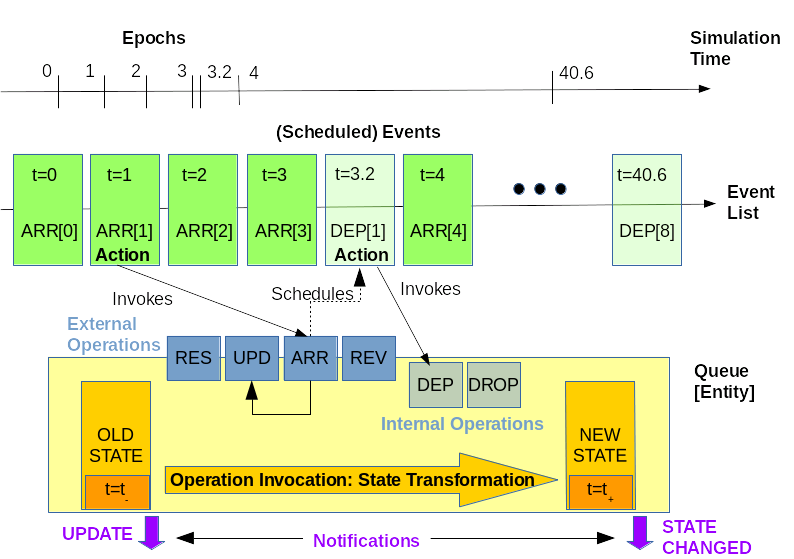
\includegraphics[width=\textwidth]{fig/SimpleSimulationOverview}
\end{figure}

In the top of the figure,
we show the simulation time and some of the epochs
from the example.
During a simulation run, the simulation time increases monotonically
as a function of "real time".
What this says is that the simulation time does not
"strictly decrease" in real time,
but at the same time,
that's pretty much the only requirement
on the relation between real time
and simulation time.
For instance,
processing the epochs between $t=0$ and $t=9$
may take several minutes in real time,
whereas epochs between $t=9$ and $t=100$
could be done in a mere second\footnote{
	This is not to say that is is impossible or even hard
	to let simulation time progress
	(roughly) at the same rate as real time,
	or at some scaled version of it.
	However, in discrete-event simulation,
	the relationship between real time and simulation time
	is generally considered unimportant.}

Below the simulation-time line,
we show the event list and some of the scheduled events
from the example.
The apparent equal distance between the events
is actually on pupose.
The event list is really not concerned with the
simulation-time differences between adjacent events.
No matter how large the time interval between an
event and its predecessor,
in between (basicaly) nothing happened:
There were not events,
and hence,
no state changes.
Going back to the figure,
we scheduled the arrival events ourselves
before processing the event list,
but we also see two "departure events"
we did not schedule.
In fact, these events were scheduled by the
queue, in response to previous events.
For instance, when job $1$ arrives at $t=1$ (simulation time),
it is taken into service immediately,
and after requesting the service time from job $1$ ($2.2$),
it schedules a {\em departure event\/} at $t=3.2$,
shown in a somewhat different color because we
did not schedule this ourselves (we are not even allowed to do so).
This shows an important aspect of the event list while processing it:
in general, the actions taken while processing the event list have
full freedom to schedule new events,
as long as they are not in the past.
This, admittedly, is not clear from the figure.
What is essential to remember is that a scheduled event
await its turn while the event list is being processed,
and the event list invokes the event's action
when it has processed all preceding events.

Assuming the event's action involves the queue in question,
we now turn our attention to the bottom part of the figure,
showing our queue from the example, the \lstinline|FCFS_B| queue.
We assume the arrival event at $t=1$ is processed by the event list,
and the net effect of this (i.e., the action of the event)
is the invokation of the arrival operation on the queue
(with the job $1$ as its argument).
As a result of this operation,
the state of the queue will transform,
and registered listeners to the queue will be informed
of the new state upon completion of the operation.
This, effectively, is the \lstinline|STATE CHANGED| notification.
In the figure this is shown with the right-pointing arrow at the bottom
from \lstinline|OLD STATE| to \lstinline|NEW STATE|,
and the \lstinline|STATE CHANGED| notification below that.

However, before doing anything,
the arrival operation invokes
the so-called \lstinline|UPDATE| operation,
which exposes the {\em old\/} state
to listeners and internally registered "hooks",
and, subsequently, increases the most essential state
property, the {\em last update time}.
By now, you should realize that
as the event list progresses in simulation time,
queues (or better, {\em entities\/})
that are not affected by the events processed
will not be bothered at all.
Yet a queue needs to assure that time-stamped operations
never lie in the past,
so they need to maintain a notion of simulation time themselves.
The importance of the \lstinline|UPDATE| notification
lies in {\em statistics gathering},
in which it is essential to know exactly
during which (non-trivial) intervals
the state of a queue did {\em not\/} change,
and the lenght of such intervals.
As long as you are not involved in statistics-gathering,
you can safely ignore these notifications,
otherwise,
you can find more details in Section \ref{chap:statistics}.

Once the \lstinline|UPDATE| operation has been
fulfilled, the \lstinline|ARR| (job arrival) operation,
in this particular case,
checks the number of jobs waiting,
and drops the arriving job if the number is $2$ ($=$\lstinline|B|)
by invoking the internal operation \lstinline|DROP|.
However, for job $1$ in the example,
it finds an empty waiting area,
and, in addition, no job being served at the server.
This means that the job is taking into service immediately
(the \lstinline|START| internal operation),
and since the required service time is non-zero,
the queue schedules a {\em departure event\/}
at $t=3.2$.
The departur event, in turn,
will invoke the internal \lstinline|DEP| (job departure)
event because of which the job
will eventually depart from the queueing system.

So, what more is there to say.
Well, we seem to have so called {\em external\/}
and {\em internal\/} operations,
the latter of which we cannot schedule ourselves
(departures, drops, $\ldots$).
In a way, the external operations allow us
to subject a queue to some kind of {\em workload\/}
consisting of arriving jobs
(as well as of, yet undescribed, other external operations on the queue).
The internal operations, on the other hand,
are always involved from within the queue itself,
either as a response to a scheduled event,
or as a response to an invocation of an external operation
in combination with a state condition
(e.g., the arrival of a job while $2$ jobs are already waiting
causes the internal \lstinline|DROP| operation to be invoked).

\section{The \texttt{Update} Operation}
\label{sec:guided:update}

In the previous section we introduced the
\lstinline|UPDATE| and \lstinline|STATE CHANGED|
notifications,
and explained that on a \lstinline|SimEntity|,
every state-change must be reported,
and that the \lstinline|UPDATE| notification
exposes the old state of the entity
for (for instance) statistics gathering.
However, there also exits an \lstinline|Update|
operation.
Its function is to set the \lstinline|LastUpdateTime|
state property of the entity.
The example shown in
Listing \ref{simExample1_update_main}
with output
shown in Listing \ref{simExample1_update_out}
demonstrates its use,
again using utility methods
for scheduling.
As the output shows,
there seems to be little use in the \lstinline|Update|
operation; it just updates the time at $t=8.5$ and $t=1000$.
The reason why you would ever want to use \lstinline|Update|
is a bit involved,
and deferred until Chapter \ref{chap:entities-queues-jobs}.
However, we included this example to demonstrate
that the end-time of the simulation can be
controlled through scheduling an \lstinline|Update|
operation.
In the next section, we will delve a little deeper
into the end-time of a simulation.

\begin{lstfloat}
	\begin{lstlisting}[
	caption={The use of the \texttt{Update} operation.},
	label=simExample1_update_main,
	basicstyle=\tiny]
	
	final SimEventList el = new DefaultSimEventList ();
	final int bufferSize = 2;
	final FCFS_B queue = new FCFS_B (el, bufferSize);
	queue.registerStdOutSimEntityListener ();
	for (int j = 0; j < 4; j++)
	{
	final double jobServiceTime = (double) 2.2 * j;
	final double jobArrivalTime = (double) j;
	final String jobName = Integer.toString (j);
	final SimJob job = new DefaultSimJob (null, jobName, jobServiceTime);
	SimJQEventScheduler.scheduleJobArrival (job, queue, jobArrivalTime);
	}
	SimEntityEventScheduler.scheduleUpdate (el, queue, 8.5);
	SimEntityEventScheduler.scheduleUpdate (el, queue, 1000.0);
	el.run ();
	
	\end{lstlisting}
\end{lstfloat}

\begin{lstfloat}
	\begin{lstlisting}[
	caption={The output of Listing \ref{simExample1_update_main}.},
	label=simExample1_update_out,
	basicstyle=\tiny]
	
	StdOutSimEntityListener t=0.0, entity=FCFS_B[2]: UPDATE.
	StdOutSimEntityListener t=0.0, entity=FCFS_B[2]: STATE CHANGED:
	=> ARRIVAL [Arr[0]@FCFS_B[2]]
	=> START [Start[0]@FCFS_B[2]]
	=> DEPARTURE [Dep[0]@FCFS_B[2]]
	StdOutSimEntityListener t=1.0, entity=FCFS_B[2]: UPDATE.
	StdOutSimEntityListener t=1.0, entity=FCFS_B[2]: STATE CHANGED:
	=> ARRIVAL [Arr[1]@FCFS_B[2]]
	=> START [Start[1]@FCFS_B[2]]
	=> STA_FALSE [StartArmed[false]@FCFS_B[2]]
	StdOutSimEntityListener t=2.0, entity=FCFS_B[2]: UPDATE.
	StdOutSimEntityListener t=2.0, entity=FCFS_B[2]: STATE CHANGED:
	=> ARRIVAL [Arr[2]@FCFS_B[2]]
	StdOutSimEntityListener t=3.0, entity=FCFS_B[2]: UPDATE.
	StdOutSimEntityListener t=3.0, entity=FCFS_B[2]: STATE CHANGED:
	=> ARRIVAL [Arr[3]@FCFS_B[2]]
	StdOutSimEntityListener t=3.2, entity=FCFS_B[2]: UPDATE.
	StdOutSimEntityListener t=3.2, entity=FCFS_B[2]: STATE CHANGED:
	=> DEPARTURE [Dep[1]@FCFS_B[2]]
	=> START [Start[2]@FCFS_B[2]]
	StdOutSimEntityListener t=7.6000000000000005, entity=FCFS_B[2]: UPDATE.
	StdOutSimEntityListener t=7.6000000000000005, entity=FCFS_B[2]: STATE CHANGED:
	=> DEPARTURE [Dep[2]@FCFS_B[2]]
	=> START [Start[3]@FCFS_B[2]]
	StdOutSimEntityListener t=8.5, entity=FCFS_B[2]: UPDATE.
	StdOutSimEntityListener t=14.200000000000001, entity=FCFS_B[2]: UPDATE.
	StdOutSimEntityListener t=14.200000000000001, entity=FCFS_B[2]: STATE CHANGED:
	=> DEPARTURE [Dep[3]@FCFS_B[2]]
	=> STA_TRUE [StartArmed[true]@FCFS_B[2]]
	StdOutSimEntityListener t=1000.0, entity=FCFS_B[2]: UPDATE.
	
	\end{lstlisting}
\end{lstfloat}

In summary:
\begin{itemize}
  \item Queues and jobs are collectively referred to as simulation {\em entities}.
  \item Simulation entities always start in a known type-specific {\em default state},
          also referred to their \lstinline|RESET STATE| upon construction
          and upon performing their \lstinline|RESET| operation.
  \item Simulation entities must always report any change to their state through
	  \lstinline|STATE CHANGED| notifications to registered {\em listeners}.
  \item Simulation entities only change their state
          as a result of the invocation of a well-defined
          {\em operation\/} on the entity.
        The operation can be external (like \lstinline-ARRIVAL-)
          or internal (like \lstinline-START-, \lstinline-DROP-, and \lstinline-DEPARTURE-).
  \item Any operation invocation takes zero (simulation) time to perform.
        Upon invocation of an operation, the new simulation time has to be supplied
          by the caller.
        With the exception of the \lstinline|RESET| operation,
          the new time provided must not be strictly smaller than the
          time of the previous invocation (of {\em any\/} operation).
  \item Before even starting the transformation from an old state into a new state,
	  simulation entities must always expose their {\em old\/} state
	  with a \lstinline|UPDATE| notification.
  \item Depending on the registered listener,
	  a simulation entity also fires {\em courtesy\/} notifications,
          revealing only a specific aspect of the state change.
        Courtesy notifications are {\em always\/} fired {\em after\/}
          the applicable \lstinline|STATE CHANGED| notification.
\end{itemize}

\section{Resetting Entities}

Every simulation entity (queue or job) supports the
external \lstinline-RESET- operation
that puts the entity into its {\em default\/} or
{\em reset\/} state.
It is the only operation that is allowed to
set {\em back\/} the time.
The new time on the entity is taken from the event list,
or to $-\infty$ if no event list is available.

The \lstinline-RESET- state of an entity depends
on the type of entity,
but it must be clearly specified.
It is, however, subject to strict rules,
as shown in Tables
\ref{resetStateSettings-queue}
and
\ref{resetStateSettings-job}.
For instance,
in the \lstinline|RESET| state,
a queue is empty (no jobs visiting).
The \lstinline|QueueAccessVacation| and
\lstinline|ServerAccessCredits|
properties will be decribed shortly
in the next sections.
In its \lstinline|RESET| state,
a job is not visiting any queue;
its \lstinline|Queue| propery is \lstinline|null|.
Beware however,
that queues are mandatorily attached to the event list,
whereas for jobs this is not required.
A queue will therefore set
the \lstinline|Queue| property to \lstinline|null|
for the jobs that it forcibly removes.

\begin{table}[h]
	\caption{Mandatory settings in the \texttt{RESET} state
		of a queue.}
	\label{resetStateSettings-queue}
	\begin{center}
		\begin{tabular}{|l|l|l|}
			\hline
			Property & Type & Default Value \\ \hline
			\lstinline|LastUpdateDate|      & \lstinline|double|      & From event list or $-\infty$.               \\ \hline
			\lstinline|Jobs|                & \lstinline|Set<SimJob>| & Empty set.                                  \\ \hline
			\lstinline|QueueAccessVacation| & \lstinline|boolean|     & \lstinline|false|.                          \\ \hline
			\lstinline|ServerAccessCredits| & \lstinline|int|         & \lstinline|Integer.MAX_VALUE| (==$\infty$). \\ \hline
			\lstinline|StartArmed|          & \lstinline|int|         & Depends on \lstinline|SimQueue| type.       \\ \hline
		\end{tabular}
	\end{center}
\end{table}

\begin{table}[h]
	\caption{Mandatory settings in the \texttt{RESET} state
		of a job.}
	\label{resetStateSettings-job}
	\begin{center}
		\begin{tabular}{|l|l|l|}
			\hline
			Property & Type & Default Value \\ \hline
			\lstinline|LastUpdateDate|      & \lstinline|double|      & From event list or $-\infty$.               \\ \hline
			\lstinline|Queue|               & \lstinline|SimQueue|    & \lstinline|null|.                           \\ \hline
		\end{tabular}
	\end{center}
\end{table}

\section{Summary of the \texttt{SimEntity} Interfaces}
\label{sec:guided:simentity-model}

In this section,
having seen almost all aspects of \lstinline|SimEntity|s,
\lstinline|SimJob|s,
and \lstinline|SimQueue|s,
we summarize their state and behavior.
We have two purposes in mind:
\begin{itemize}
	\item To present the material presented thus far in a format
	that allows you to assert your understanding
	of the fundamental concepts in \lstinline|jqueues|
	and \lstinline|jsimulation|.
	\item To present the interfaces in a compact overview format
	that can be used as a reference.
	Really, at this point we have covered almost every aspect
	of entities, queues, and jobs, and their listeners.
	The remainder of this Chapter will focus at some
	left-overs and an important class of queues
	named {\em composite queues}.
	The remainder of this entire book is really
	about explaining rigorously the abstract interfaces
	and the specific concrete types
	of queues (mostly), jobs and listeners,
	and about how you can build your own.
	In other words, the summary presented in this section
	is quite complete already,
	hence it is worth using as a reference.
\end{itemize}


%\chapter{Listeners}
%\label{chap:listeners}
%In \lstinline|jqueues|, monitoring the progress of a running simulation,
  or perhaps calculating statistiscs on it,
  starts with chosing the proper {\em listeners}.
During the simulation,
  queues and jobs, from hereon collectively referred to as {\em entities},
  are obliged to notify registered listeners of (at least) {\em all\/}
  changes to their states.
A listener is a \lstinline|Java| object implementing the required methods
  allowing such notifications from the entity.

Since in most practical simulation studies,
the ambition level is somewhat higher that showing events on \lstinline|System.out|,
we will delve somewhat deeper into listeners types and how
to create, modify and register them.

In the example of Listing \ref{simExample1_main},
  we used a convenience method \lstinline|registerStdOutSimQueueListener|
  to register a listener at the \lstinline|FCFS_B| queue
  that simply writes the details of such notifications
  to the standard output, \lstinline|Sytem.out| in \lstinline|Java|.
This is extremely handy for initial testing of a simulation,
  but in almost all cases,
  a more sophisticated listener is required;
  one you have to create yourself.
Luckily, \lstinline|jqueues| comes with a large collection of
  listener implementations, each for a specific purpose, that
  you can modify to suit your needs.

Restricting ourselves for the moment to queue listeners,
  we can create and register
  our own listener that reports to \lstinline|System.out|
  in the code in Listing \ref{simExample1_main}:

\begin{lstfloat}
\begin{lstlisting}[
  caption={Creating and registering a listener.},
  label=simExample1_listener1,
  basicstyle=\tiny]

  final SimQueueListener listener = new StdOutSimQueueListener ();
  queue.registerSimEntityListener (listener);

\end{lstlisting}
\end{lstfloat}

Running the program of \ref{simExample1_main} again with
  this modified code fragment will yield (roughly)
  the same output, so we have not gained anything so far.
However,
  a \lstinline|StdOutSimQueueListener| allows
  all (notification) methods to be overridden,
  so we can, for instance,
  suppress certain notifications in the output like this:

\begin{lstfloat}
\begin{lstlisting}[
  caption={Suppressing specific notifications in a \texttt{StdOutSimQueueListener}.},
  label=simExample1_listener1_suppress,
  basicstyle=\tiny]

    final SimQueueListener listener = new StdOutSimQueueListener ()
    {
      
      @Override
      public void notifyStateChanged (double time, SimEntity entity, List notifications) {}

      @Override
      public void notifyUpdate (double time, SimEntity entity) {}
      
      @Override
      public void notifyStartQueueAccessVacation (double time, SimQueue queue) {}

      @Override
      public void notifyStopQueueAccessVacation (double time, SimQueue queue) {}

      @Override
      public void notifyNewStartArmed (double time, SimQueue queue, boolean startArmed) {}
      
      @Override
      public void notifyOutOfServerAccessCredits (double time, SimQueue queue) {}

      @Override
      public void notifyRegainedServerAccessCredits (double time, SimQueue queue) {}

    };
    queue.registerSimEntityListener (listener);

\end{lstlisting}
\end{lstfloat}

In Listing \ref{simExample1_listener1_suppress},
  we modify the \lstinline|StdOutSimQueueListener| by overriding
  the notification methods for
  server-access credits
  and queue-access vacations
  (which we do have not described yet),
  for the \lstinline|StartArmed|-related notifications
  and replacing them with empty methods,
  effectively suppressing their respective
  output on \lstinline|System.out|.
In addition,
  we suppress the \lstinline|UPDATE| and \lstinline|STATE CHANGED|
  notifications.
Our modified listener yields the following output:

\begin{lstfloat}
\begin{lstlisting}[
  caption={Example output of Listing \ref{simExample1_main} with the modified listener of Listing
  \ref{simExample1_listener1_suppress}},
  label=simExample1_listener1_out,
  basicstyle=\tiny]

 t=0.0, queue=FCFS_B[2]: ARRIVAL of job 0.
 t=0.0, queue=FCFS_B[2]: START of job 0.
 t=0.0, queue=FCFS_B[2]: DEPARTURE of job 0.
 t=1.0, queue=FCFS_B[2]: ARRIVAL of job 1.
 t=1.0, queue=FCFS_B[2]: START of job 1.
 t=2.0, queue=FCFS_B[2]: ARRIVAL of job 2.
 t=3.0, queue=FCFS_B[2]: ARRIVAL of job 3.
 t=3.2, queue=FCFS_B[2]: DEPARTURE of job 1.
 t=3.2, queue=FCFS_B[2]: START of job 2.
 t=4.0, queue=FCFS_B[2]: ARRIVAL of job 4.
 t=5.0, queue=FCFS_B[2]: ARRIVAL of job 5.
 t=5.0, queue=FCFS_B[2]: DROP of job 5.
 t=6.0, queue=FCFS_B[2]: ARRIVAL of job 6.
 t=6.0, queue=FCFS_B[2]: DROP of job 6.
 t=7.0, queue=FCFS_B[2]: ARRIVAL of job 7.
 t=7.0, queue=FCFS_B[2]: DROP of job 7.
 t=7.6000000000000005, queue=FCFS_B[2]: DEPARTURE of job 2.
 t=7.6000000000000005, queue=FCFS_B[2]: START of job 3.
 t=8.0, queue=FCFS_B[2]: ARRIVAL of job 8.
 t=9.0, queue=FCFS_B[2]: ARRIVAL of job 9.
 t=9.0, queue=FCFS_B[2]: DROP of job 9.
 t=14.200000000000001, queue=FCFS_B[2]: DEPARTURE of job 3.
 t=14.200000000000001, queue=FCFS_B[2]: START of job 4.
 t=23.0, queue=FCFS_B[2]: DEPARTURE of job 4.
 t=23.0, queue=FCFS_B[2]: START of job 8.
 t=40.6, queue=FCFS_B[2]: DEPARTURE of job 8.

\end{lstlisting}
\end{lstfloat}

If, on the other hand, your {\em only\/} interest is in the
  fundamental \lstinline|RESET|, \lstinline|UPDATE| and \lstinline|STATE CHANGED|
  notifications,
  you can register a \lstinline|StdOutSimEntityListener|
  as shown in Listing \ref{simExample1_listener2_1}
  or, simpler but equivalent, Listing \ref{simExample1_listener2_2},
  and their corresponding output in Listing \ref{simExample1_listener2_out}.

\begin{lstfloat}
\begin{lstlisting}[
  caption={Creating and registering a \texttt{StdOutSimEntityListener}.},
  label=simExample1_listener2_1,
  basicstyle=\tiny]

  final SimEntityListener listener = new StdOutSimEntityListener ();
  queue.registerSimEntityListener (listener);

\end{lstlisting}
\end{lstfloat}


\begin{lstfloat}
\begin{lstlisting}[
  caption={Using \texttt{registerStdOutSimEntityListener}.},
  label=simExample1_listener2_2,
  basicstyle=\tiny]

  queue.registerStdOutSimEntityListener ();

\end{lstlisting}
\end{lstfloat}

\begin{lstfloat}
\begin{lstlisting}[
  caption={Example output of Listing \ref{simExample1_main} with the modified listener of Listings
  \ref{simExample1_listener2_1} or \ref{simExample1_listener2_2}},
  label=simExample1_listener2_out,
  basicstyle=\tiny]

StdOutSimEntityListener t=0.0, entity=FCFS_B[2]: UPDATE.
StdOutSimEntityListener t=0.0, entity=FCFS_B[2]: STATE CHANGED:
  => ARRIVAL [Arr[0]@FCFS_B[2]]
  => START [Start[0]@FCFS_B[2]]
  => DEPARTURE [Dep[0]@FCFS_B[2]]
StdOutSimEntityListener t=1.0, entity=FCFS_B[2]: UPDATE.
StdOutSimEntityListener t=1.0, entity=FCFS_B[2]: STATE CHANGED:
  => ARRIVAL [Arr[1]@FCFS_B[2]]
  => START [Start[1]@FCFS_B[2]]
  => STA_FALSE [StartArmed[false]@FCFS_B[2]]
StdOutSimEntityListener t=2.0, entity=FCFS_B[2]: UPDATE.
StdOutSimEntityListener t=2.0, entity=FCFS_B[2]: STATE CHANGED:
  => ARRIVAL [Arr[2]@FCFS_B[2]]
StdOutSimEntityListener t=3.0, entity=FCFS_B[2]: UPDATE.
StdOutSimEntityListener t=3.0, entity=FCFS_B[2]: STATE CHANGED:
  => ARRIVAL [Arr[3]@FCFS_B[2]]
StdOutSimEntityListener t=3.2, entity=FCFS_B[2]: UPDATE.
StdOutSimEntityListener t=3.2, entity=FCFS_B[2]: STATE CHANGED:
  => DEPARTURE [Dep[1]@FCFS_B[2]]
  => START [Start[2]@FCFS_B[2]]
StdOutSimEntityListener t=4.0, entity=FCFS_B[2]: UPDATE.
StdOutSimEntityListener t=4.0, entity=FCFS_B[2]: STATE CHANGED:
  => ARRIVAL [Arr[4]@FCFS_B[2]]
StdOutSimEntityListener t=5.0, entity=FCFS_B[2]: UPDATE.
StdOutSimEntityListener t=5.0, entity=FCFS_B[2]: STATE CHANGED:
  => ARRIVAL [Arr[5]@FCFS_B[2]]
  => DROP [Drop[5]@FCFS_B[2]]
StdOutSimEntityListener t=6.0, entity=FCFS_B[2]: UPDATE.
StdOutSimEntityListener t=6.0, entity=FCFS_B[2]: STATE CHANGED:
  => ARRIVAL [Arr[6]@FCFS_B[2]]
  => DROP [Drop[6]@FCFS_B[2]]
StdOutSimEntityListener t=7.0, entity=FCFS_B[2]: UPDATE.
StdOutSimEntityListener t=7.0, entity=FCFS_B[2]: STATE CHANGED:
  => ARRIVAL [Arr[7]@FCFS_B[2]]
  => DROP [Drop[7]@FCFS_B[2]]
StdOutSimEntityListener t=7.6000000000000005, entity=FCFS_B[2]: UPDATE.
StdOutSimEntityListener t=7.6000000000000005, entity=FCFS_B[2]: STATE CHANGED:
  => DEPARTURE [Dep[2]@FCFS_B[2]]
  => START [Start[3]@FCFS_B[2]]
StdOutSimEntityListener t=8.0, entity=FCFS_B[2]: UPDATE.
StdOutSimEntityListener t=8.0, entity=FCFS_B[2]: STATE CHANGED:
  => ARRIVAL [Arr[8]@FCFS_B[2]]
StdOutSimEntityListener t=9.0, entity=FCFS_B[2]: UPDATE.
StdOutSimEntityListener t=9.0, entity=FCFS_B[2]: STATE CHANGED:
  => ARRIVAL [Arr[9]@FCFS_B[2]]
  => DROP [Drop[9]@FCFS_B[2]]
StdOutSimEntityListener t=14.200000000000001, entity=FCFS_B[2]: UPDATE.
StdOutSimEntityListener t=14.200000000000001, entity=FCFS_B[2]: STATE CHANGED:
  => DEPARTURE [Dep[3]@FCFS_B[2]]
  => START [Start[4]@FCFS_B[2]]
StdOutSimEntityListener t=23.0, entity=FCFS_B[2]: UPDATE.
StdOutSimEntityListener t=23.0, entity=FCFS_B[2]: STATE CHANGED:
  => DEPARTURE [Dep[4]@FCFS_B[2]]
  => START [Start[8]@FCFS_B[2]]
StdOutSimEntityListener t=40.6, entity=FCFS_B[2]: UPDATE.
StdOutSimEntityListener t=40.6, entity=FCFS_B[2]: STATE CHANGED:
  => DEPARTURE [Dep[8]@FCFS_B[2]]
  => STA_TRUE [StartArmed[true]@FCFS_B[2]]

\end{lstlisting}
\end{lstfloat}

In most practical cases,
  you will need a listener that does a bit more than reporting to \lstinline|System.out|.
Of course, you can override the methods in \lstinline|StdOutSimQueueListener|
  to fit your purposes, but a better way is to use a \lstinline|DefaultSimQueueListener|,
  or, if you just want to process the fundamental notification (\lstinline|RESET|,
  \lstinline|UPDATE| and \lstinline|STATE CHANGED|),
  a \lstinline|DefaultSimEntityListener|.
Both listener type are concrete,
  but all required method implementations are empty.
In our next example,
  we take a \lstinline|DefaultSimQueueListener|
  and modify it in order to calculate the average
  job {\em sojourn\/} time.
This time,
  we create a separate \lstinline|class| named \lstinline|JobSojournTimeListener|
  for the listener,
  shown in Listing \ref{simExample1_avgSojournTime_class}.

\begin{lstfloat}
\begin{lstlisting}[
  caption={A (somewhat naive) queue listener that calculates the average job sojourn time.},
  label=simExample1_avgSojournTime_class,
  basicstyle=\tiny]

public class JobSojournTimeListener
extends DefaultSimQueueListener
{

  private final Map<SimJob, Double> jobArrTimes = new HashMap<> ();

  private int jobsPassed = 0;
  private double cumJobSojournTime = 0;
  
  @Override
  public void notifyArrival (double time, SimJob job, SimQueue queue)
  {
    if (this.jobArrTimes.containsKey (job))
      throw new IllegalStateException ();
    this.jobArrTimes.put (job, time);
  }
  
  @Override
  public void notifyDeparture (double time, SimJob job, SimQueue queue)
  {
    if (! this.jobArrTimes.containsKey (job))
      throw new IllegalStateException ();
    final double jobSojournTime = time - this.jobArrTimes.get (job);
    if (jobSojournTime < 0)
      throw new IllegalStateException ();
    this.jobArrTimes.remove (job);
    this.jobsPassed++;
    this.cumJobSojournTime += jobSojournTime;
  }

  @Override
  public void notifyDrop (double time, SimJob job, SimQueue queue)
  {
    notifyDeparture (time, job, queue);
  }
  
  public double getAvgSojournTime ()
  {
    if (this.jobsPassed == 0)
      return Double.NaN;
    return this.cumJobSojournTime / this.jobsPassed;
  }
  
}

\end{lstlisting}
\end{lstfloat}

In the class, we override the (courtesy) notifications for job arrivals,
  departures and drops.
When a job arrives, its arrival time is put into a private \lstinline|Map| (\lstinline|jobArrTimes|)
  for later reference.
When a job departs or is dropped,
  we retrieve its arrival time,
  calculate its sojourn time,
  and add the result to the cumulative sum
  of sojourn times, \lstinline|cumJobSojournTime|.
In order to later interpret this value,
  we also have to maintain the number of jobs passed
  in a private field \lstinline|jobsPassed|.
At any time,
  the class provides the average sojourn time (over all jobs {\em passed\/})
  through its \lstinline|getAvgSojournTime| method.
The calculation involved is trivial;
  the method returns \lstinline|Double.NaN| when
  no jobs have passed.

The use of \lstinline|JobSojournTimeListener| and the corresponding output
  are shown in Listings \ref{simExample1_avgSojournTime_main}
  and \ref{simExample1_avgSojournTime_out}, respectively.

\begin{lstfloat}
\begin{lstlisting}[
  caption={Our \texttt{FCFS\_B} example
           with the custom \texttt{JobSojournTimeListener}.},
  label=simExample1_avgSojournTime_main,
  basicstyle=\tiny]

    final SimEventList el = new DefaultSimEventList ();
    final int bufferSize = 2;
    final FCFS_B queue = new FCFS_B (el, bufferSize);
    final JobSojournTimeListener listener = new JobSojournTimeListener ();
    queue.registerSimEntityListener (listener);
    for (int j = 0; j < 10; j++)
    {
      final double jobServiceTime = (double) 2.2 * j;
      final double jobArrivalTime = (double) j;
      final String jobName = Integer.toString (j);
      final SimJob job = new DefaultSimJob (null, jobName, jobServiceTime);
      SimJQEventScheduler.scheduleJobArrival (job, queue, jobArrivalTime);
    }
    el.run ();
    System.out.println ("Average job sojourn time is " + listener.getAvgSojournTime () + ".");

\end{lstlisting}
\end{lstfloat}

\begin{lstfloat}
\begin{lstlisting}[
  caption={The output of Listing \ref{simExample1_avgSojournTime_main}.},
  label=simExample1_avgSojournTime_out,
  basicstyle=\tiny]

Average job sojourn time is 7.06.

\end{lstlisting}
\end{lstfloat}

Before going into details on the average sojourn time reported,
  we want to stress that our implementation of
  \lstinline|JobSojournTimeListener| is far from complete and even erroneous,
  although it works correctly in this specific (use) case.
For instance, it fails to consider the fact that jobs may
  {\em not\/} leave the queue (in whatever way).
Such jobs are named {\em sticky\/} jobs,
  and in a true application we would have to consider them.
Second,
  apart from \lstinline|DROP| and \lstinline|DEPARTURE|,
  there are other means by which a job
  can depart the queueing system
  (in particular, {\em revocations\/}).
%   see Section \ref{sec:guided:revocations}).
Third,
  the listener ignores \lstinline|RESET|
  notifications from the queue;
  a critical error as we shall see later.
%  as will become
%  clear later in Section \ref{sec:guided:reset}.
We will not further discuss these and other complications here,
  because our primary intention is to show you
  the mechanisms for creating and modifying listeners.
We just want to point out that the design of {\em robust\/}
  statistical listeners is more complicated that shown here.
We provide a thorough treatment in Chapter \ref{chap:statistics}.

Returning to the reported average job sojourn time.
Is it correct?
Well, in order to verify, we have no choice but to carefully analyze
  the behavior of the \lstinline|FCFS_B| queue under the given
  workload of jobs, as given in Table \ref{simExample1_analysis}.
The table shows for each job its
  job number (Job),
  arival time (Arr),
  required service time (ReQ),
  jobs waiting upon its arrival (WQA),
  start time (Start, if applicable),
  exit time (either due to departure or due to dropping),
  sojourn time (exit time minus arrival time),
  and remarks if applicable.
The final rows
  show the sum (TOT) and the average (AVG)
  of the required service times and
  the sojourn times,
  thus validating the result.

\begin{table}[h]
\caption{Analysis of job sojourn times in Listing \ref{simExample1_main}.}
\label{simExample1_analysis}
\begin{center}
\begin{tabular}{|l|l|r|l|r|r|r|l|}
\hline
Job & Arr & ReqS & WQA & Start & Exit & Sojourn & Remark \\
\hline
\hline
0 & 0.0 &  0.0 & $\{      \}$ & 0.0  &  0.0 &  0.0 & Exits immediately. \\ \hline
1 & 1.0 &  2.2 & $\{      \}$ & 1.0  &  3.2 &  2.2 &                    \\ \hline
2 & 2.0 &  4.4 & $\{      \}$ & 3.2  &  7.6 &  5.6 &                    \\ \hline
3 & 3.0 &  6.6 & $\{ 2    \}$ & 7.6  & 14.2 & 11.2 &                    \\ \hline
4 & 4.0 &  8.8 & $\{ 3    \}$ & 14.2 & 23.0 & 19.0 &                    \\ \hline
5 & 5.0 & 11.0 & $\{ 3, 4 \}$ & -    &  5.0 &  0.0 & Dropped.           \\ \hline
6 & 6.0 & 13.2 & $\{ 3, 4 \}$ & -    &  6.0 &  0.0 & Dropped.           \\ \hline
7 & 7.0 & 15.4 & $\{ 3, 4 \}$ & -    &  7.0 &  0.0 & Dropped.           \\ \hline
8 & 8.0 & 17.6 & $\{ 4    \}$ & 23.0 & 40.6 & 32.6 &                    \\ \hline
9 & 9.0 & 19.8 & $\{ 4, 8 \}$ & -    &  9.0 &  0.0 & Dropped.           \\ \hline
\hline
TOT   & & 99.0 &              &      &      & 70.6 &                    \\ \hline
\hline
AVG   & &  9.9 &              &      &      & 7.06 &                    \\ \hline
\hline
\end{tabular}
\end{center}
\end{table}



%\chapter{Generic Queue Model}
%\label{chap:generic-queue-model}
%\section{Summary}

\begin{itemize}
	\item In simulation of queueing systems,
	the center of attention is a simulation entity,
	an object with a state subject to (the actions of) simulation events.
	\item In \lstinline|jqueues|, simulation entities are represented
	as \lstinline|SimEntity| objects.
	In the present release,
	a \lstinline|SimEntity| is either a \lstinline|SimJob|
	(job) or \lstinline|SimQueue| (or their abstract joint interface,
	\lstinline|SimJQ|).
	However, other types of \lstinline|SimEntity| may be added in a future release.
	\item A \lstinline|SimEntity| has the obligation to report
	changes to its state (as a result of event-list processing)
	to registered listeners,
	which are of type \lstinline|SimEntityListener|.
	Listeners to a \lstinline|SimEntity| can be registered and
	unregistered at any time through the
	\lstinline|SimEntity.registerSimEntityListener|
	and \lstinline|SimEntity.unregisterSimEntityListener|
	methods, respectively.
	\item In \lstinline|jqueues|, changes to the state
	of a \lstinline|SimEntity| is always the result
	of the invocation of one of a set of well-defined
	operations on the entity.
	The specific type of \lstinline|SimEntity|
	determines the operation it supports.
	The invocation of an operation is
	almost always performed by a scheduled event.
	\item An operation can be external or internal.
	Events for internal events can only be scheduled
	by the \lstinline|SimEntity| itself.
	\item Upon reception of {\em any\/} operation invocation,
	but before doing anything,
	a \lstinline|SimEntity| fires an \lstinline|UPDATE|
	notification exposing the {\em a priori\/} state
	(i.e., the "old" state).
	\item After completion of an operation invocation,
	but {\em before\/} handing back control (to the event list),
	a \lstinline|SimEntity| fires a \lstinline|STATE CHANGED|
	notification exposing the {\em a posteriori\/} state
	(i.e., the "new" state).
	In some cases, no state-change notification is fired when
	the state did not actually change.
	\item The external operations on a \lstinline|SimQueue| are
	\lstinline|Arrive| and \lstinline|Revoke|.
	\item In \lstinline|jqueues|,
	a \lstinline|SimJob| starts a visit to a \lstinline|SimQueue|
	through the \lstinline|Arrive| operation.
	Listeners are always notified of invocations of \lstinline|Arrive|,
	even if no state change occurs on the entity.
	\item While a \lstinline|SimJob| is present (visiting) a \lstinline|SimQueue|,
	it is either in its waiting or service area.
	Upon arrival, a \lstinline|SimJob| enters the waiting area.
	Moving a \lstinline|SimJob| from the waiting to the service area
	is performed (if at all) through the internal \lstinline|START|
	operation.
	Invocations of the \lstinline|Start| operation are always notified to
	listeners, even if no state change occurs.
	\item The visit of a \lstinline|SimJob| to a \lstinline|SimQueue|
	can end in one of following three ways: (1) Through departure
	(the internal \lstinline|Depart| operation), (2) through dropping
	(the internal \lstinline|Drop| operation), or (3) through revocation
	(the external \lstinline|Revoke| operation or the internal \lstinline|AutoRevoke| operation).
	Whatever way the \lstinline|SimJob| leaves, it can be from the waiting
	and service area.
	Invocations of the \lstinline|Drop| operation are always notified to
	listeners, even if no state change occurs.
	\item A job that is present on a queue, but never leaves during a simulation run
	is named a sticky job.
\end{itemize}

\section{The \texttt{UPDATE} and \texttt{STATE CHANGED} Notifications}

As you may have spotted,
events are actually reported twice,
once as part of a \lstinline|STATE CHANGED| notification,
followed by a separate notification specific to the event type
(\lstinline-ARRIVAL-, \lstinline-DEPARTURE-, etc.).
As a matter of fact, these separate notifications are merely a courtesy
of the queue as it is only required to issue
\lstinline|UPDATE|, \lstinline|STATE CHANGED| and \lstinline|RESET| notifications.

In order to understand this,
  we must realize that in {\em any\/} discrete-event simulation,
  the entities (like queues) involved possess an individual {\em state\/}
  that can only change at discrete moments in time (the {\em epochs\/}),
  and as a result of an {\em operation\/} on the entity at that time.
This is explained graphically in Figure \ref{fig:SimpleSimulationOverview}.

\begin{figure}[h]
	\label{fig:SimpleSimulationOverview}
	\caption{The relations between simulation time, epochs,
		the event list, scheduled events, and actions,
		as well their impact on notifications from
		and operations on
		(the state of) an entity.}
	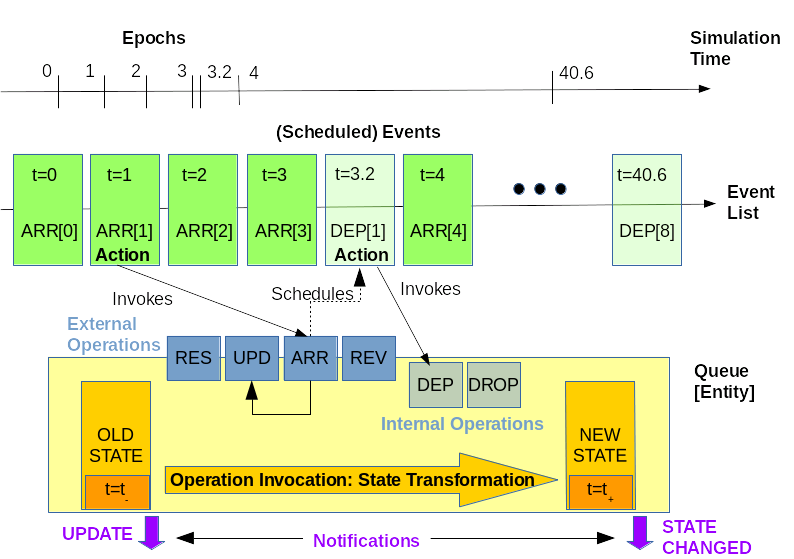
\includegraphics[width=\textwidth]{fig/SimpleSimulationOverview}
\end{figure}

In the top of the figure,
we show the simulation time and some of the epochs
from the example.
During a simulation run, the simulation time increases monotonically
as a function of "real time".
What this says is that the simulation time does not
"strictly decrease" in real time,
but at the same time,
that's pretty much the only requirement
on the relation between real time
and simulation time.
For instance,
processing the epochs between $t=0$ and $t=9$
may take several minutes in real time,
whereas epochs between $t=9$ and $t=100$
could be done in a mere second\footnote{
	This is not to say that is is impossible or even hard
	to let simulation time progress
	(roughly) at the same rate as real time,
	or at some scaled version of it.
	However, in discrete-event simulation,
	the relationship between real time and simulation time
	is generally considered unimportant.}

Below the simulation-time line,
we show the event list and some of the scheduled events
from the example.
The apparent equal distance between the events
is actually on pupose.
The event list is really not concerned with the
simulation-time differences between adjacent events.
No matter how large the time interval between an
event and its predecessor,
in between (basicaly) nothing happened:
There were not events,
and hence,
no state changes.
Going back to the figure,
we scheduled the arrival events ourselves
before processing the event list,
but we also see two "departure events"
we did not schedule.
In fact, these events were scheduled by the
queue, in response to previous events.
For instance, when job $1$ arrives at $t=1$ (simulation time),
it is taken into service immediately,
and after requesting the service time from job $1$ ($2.2$),
it schedules a {\em departure event\/} at $t=3.2$,
shown in a somewhat different color because we
did not schedule this ourselves (we are not even allowed to do so).
This shows an important aspect of the event list while processing it:
in general, the actions taken while processing the event list have
full freedom to schedule new events,
as long as they are not in the past.
This, admittedly, is not clear from the figure.
What is essential to remember is that a scheduled event
await its turn while the event list is being processed,
and the event list invokes the event's action
when it has processed all preceding events.

Assuming the event's action involves the queue in question,
we now turn our attention to the bottom part of the figure,
showing our queue from the example, the \lstinline|FCFS_B| queue.
We assume the arrival event at $t=1$ is processed by the event list,
and the net effect of this (i.e., the action of the event)
is the invokation of the arrival operation on the queue
(with the job $1$ as its argument).
As a result of this operation,
the state of the queue will transform,
and registered listeners to the queue will be informed
of the new state upon completion of the operation.
This, effectively, is the \lstinline|STATE CHANGED| notification.
In the figure this is shown with the right-pointing arrow at the bottom
from \lstinline|OLD STATE| to \lstinline|NEW STATE|,
and the \lstinline|STATE CHANGED| notification below that.

However, before doing anything,
the arrival operation invokes
the so-called \lstinline|UPDATE| operation,
which exposes the {\em old\/} state
to listeners and internally registered "hooks",
and, subsequently, increases the most essential state
property, the {\em last update time}.
By now, you should realize that
as the event list progresses in simulation time,
queues (or better, {\em entities\/})
that are not affected by the events processed
will not be bothered at all.
Yet a queue needs to assure that time-stamped operations
never lie in the past,
so they need to maintain a notion of simulation time themselves.
The importance of the \lstinline|UPDATE| notification
lies in {\em statistics gathering},
in which it is essential to know exactly
during which (non-trivial) intervals
the state of a queue did {\em not\/} change,
and the lenght of such intervals.
As long as you are not involved in statistics-gathering,
you can safely ignore these notifications,
otherwise,
you can find more details in Section \ref{chap:statistics}.

Once the \lstinline|UPDATE| operation has been
fulfilled, the \lstinline|ARR| (job arrival) operation,
in this particular case,
checks the number of jobs waiting,
and drops the arriving job if the number is $2$ ($=$\lstinline|B|)
by invoking the internal operation \lstinline|DROP|.
However, for job $1$ in the example,
it finds an empty waiting area,
and, in addition, no job being served at the server.
This means that the job is taking into service immediately
(the \lstinline|START| internal operation),
and since the required service time is non-zero,
the queue schedules a {\em departure event\/}
at $t=3.2$.
The departure event, in turn,
will invoke the internal \lstinline|DEP| (job departure)
event because of which the job
will eventually depart from the queueing system.

So, what more is there to say.
Well, we seem to have so called {\em external\/}
and {\em internal\/} operations,
the latter of which we cannot schedule ourselves
(departures, drops, $\ldots$).
In a way, the external operations allow us
to subject a queue to some kind of {\em workload\/}
consisting of arriving jobs
(as well as of, yet undescribed, other external operations on the queue).
The internal operations, on the other hand,
are always involved from within the queue itself,
either as a response to a scheduled event,
or as a response to an invocation of an external operation
in combination with a state condition
(e.g., the arrival of a job while $2$ jobs are already waiting
causes the internal \lstinline|DROP| operation to be invoked).

\section{The \texttt{Update} Operation}
\label{sec:guided:update}

In the previous section we introduced the
\lstinline|UPDATE| and \lstinline|STATE CHANGED|
notifications,
and explained that on a \lstinline|SimEntity|,
every state-change must be reported,
and that the \lstinline|UPDATE| notification
exposes the old state of the entity
for (for instance) statistics gathering.
However, there also exits an \lstinline|Update|
operation.
Its function is to set the \lstinline|LastUpdateTime|
state property of the entity.
The example shown in
Listing \ref{simExample1_update_main}
with output
shown in Listing \ref{simExample1_update_out}
demonstrates its use,
again using utility methods
for scheduling.
As the output shows,
there seems to be little use in the \lstinline|Update|
operation; it just updates the time at $t=8.5$ and $t=1000$.
The reason why you would ever want to use \lstinline|Update|
is a bit involved,
and deferred until Chapter \ref{chap:entities-queues-jobs}.
However, we included this example to demonstrate
that the end-time of the simulation can be
controlled through scheduling an \lstinline|Update|
operation.
In the next section, we will delve a little deeper
into the end-time of a simulation.

\begin{lstfloat}
	\begin{lstlisting}[
	caption={The use of the \texttt{Update} operation.},
	label=simExample1_update_main,
	basicstyle=\tiny]
	
	final SimEventList el = new DefaultSimEventList ();
	final int bufferSize = 2;
	final FCFS_B queue = new FCFS_B (el, bufferSize);
	queue.registerStdOutSimEntityListener ();
	for (int j = 0; j < 4; j++)
	{
	final double jobServiceTime = (double) 2.2 * j;
	final double jobArrivalTime = (double) j;
	final String jobName = Integer.toString (j);
	final SimJob job = new DefaultSimJob (null, jobName, jobServiceTime);
	SimJQEventScheduler.scheduleJobArrival (job, queue, jobArrivalTime);
	}
	SimEntityEventScheduler.scheduleUpdate (el, queue, 8.5);
	SimEntityEventScheduler.scheduleUpdate (el, queue, 1000.0);
	el.run ();
	
	\end{lstlisting}
\end{lstfloat}

\begin{lstfloat}
	\begin{lstlisting}[
	caption={The output of Listing \ref{simExample1_update_main}.},
	label=simExample1_update_out,
	basicstyle=\tiny]
	
	StdOutSimEntityListener t=0.0, entity=FCFS_B[2]: UPDATE.
	StdOutSimEntityListener t=0.0, entity=FCFS_B[2]: STATE CHANGED:
	=> ARRIVAL [Arr[0]@FCFS_B[2]]
	=> START [Start[0]@FCFS_B[2]]
	=> DEPARTURE [Dep[0]@FCFS_B[2]]
	StdOutSimEntityListener t=1.0, entity=FCFS_B[2]: UPDATE.
	StdOutSimEntityListener t=1.0, entity=FCFS_B[2]: STATE CHANGED:
	=> ARRIVAL [Arr[1]@FCFS_B[2]]
	=> START [Start[1]@FCFS_B[2]]
	=> STA_FALSE [StartArmed[false]@FCFS_B[2]]
	StdOutSimEntityListener t=2.0, entity=FCFS_B[2]: UPDATE.
	StdOutSimEntityListener t=2.0, entity=FCFS_B[2]: STATE CHANGED:
	=> ARRIVAL [Arr[2]@FCFS_B[2]]
	StdOutSimEntityListener t=3.0, entity=FCFS_B[2]: UPDATE.
	StdOutSimEntityListener t=3.0, entity=FCFS_B[2]: STATE CHANGED:
	=> ARRIVAL [Arr[3]@FCFS_B[2]]
	StdOutSimEntityListener t=3.2, entity=FCFS_B[2]: UPDATE.
	StdOutSimEntityListener t=3.2, entity=FCFS_B[2]: STATE CHANGED:
	=> DEPARTURE [Dep[1]@FCFS_B[2]]
	=> START [Start[2]@FCFS_B[2]]
	StdOutSimEntityListener t=7.6000000000000005, entity=FCFS_B[2]: UPDATE.
	StdOutSimEntityListener t=7.6000000000000005, entity=FCFS_B[2]: STATE CHANGED:
	=> DEPARTURE [Dep[2]@FCFS_B[2]]
	=> START [Start[3]@FCFS_B[2]]
	StdOutSimEntityListener t=8.5, entity=FCFS_B[2]: UPDATE.
	StdOutSimEntityListener t=14.200000000000001, entity=FCFS_B[2]: UPDATE.
	StdOutSimEntityListener t=14.200000000000001, entity=FCFS_B[2]: STATE CHANGED:
	=> DEPARTURE [Dep[3]@FCFS_B[2]]
	=> STA_TRUE [StartArmed[true]@FCFS_B[2]]
	StdOutSimEntityListener t=1000.0, entity=FCFS_B[2]: UPDATE.
	
	\end{lstlisting}
\end{lstfloat}

In summary:
\begin{itemize}
  \item Queues and jobs are collectively referred to as simulation {\em entities}.
  \item Simulation entities always start in a known type-specific {\em default state},
          also referred to their \lstinline|RESET STATE| upon construction
          and upon performing their \lstinline|RESET| operation.
  \item Simulation entities must always report any change to their state through
	  \lstinline|STATE CHANGED| notifications to registered {\em listeners}.
  \item Simulation entities only change their state
          as a result of the invocation of a well-defined
          {\em operation\/} on the entity.
        The operation can be external (like \lstinline-ARRIVAL-)
          or internal (like \lstinline-START-, \lstinline-DROP-, and \lstinline-DEPARTURE-).
  \item Any operation invocation takes zero (simulation) time to perform.
        Upon invocation of an operation, the new simulation time has to be supplied
          by the caller.
        With the exception of the \lstinline|RESET| operation,
          the new time provided must not be strictly smaller than the
          time of the previous invocation (of {\em any\/} operation).
  \item Before even starting the transformation from an old state into a new state,
	  simulation entities must always expose their {\em old\/} state
	  with a \lstinline|UPDATE| notification.
  \item Depending on the registered listener,
	  a simulation entity also fires {\em courtesy\/} notifications,
          revealing only a specific aspect of the state change.
        Courtesy notifications are {\em always\/} fired {\em after\/}
          the applicable \lstinline|STATE CHANGED| notification.
\end{itemize}

\section{Resetting Entities}

Every simulation entity (queue or job) supports the
external \lstinline-RESET- operation
that puts the entity into its {\em default\/} or
{\em reset\/} state.
It is the only operation that is allowed to
set {\em back\/} the time.
The new time on the entity is taken from the event list,
or to $-\infty$ if no event list is available.

The \lstinline-RESET- state of an entity depends
on the type of entity,
but it must be clearly specified.
It is, however, subject to strict rules,
as shown in Tables
\ref{resetStateSettings-queue}
and
\ref{resetStateSettings-job}.
For instance,
in the \lstinline|RESET| state,
a queue is empty (no jobs visiting).
The \lstinline|QueueAccessVacation| and
\lstinline|ServerAccessCredits|
properties will be decribed shortly
in the next sections.
In its \lstinline|RESET| state,
a job is not visiting any queue;
its \lstinline|Queue| propery is \lstinline|null|.
Beware however,
that queues are mandatorily attached to the event list,
whereas for jobs this is not required.
A queue will therefore set
the \lstinline|Queue| property to \lstinline|null|
for the jobs that it forcibly removes.

\begin{table}[h]
	\caption{Mandatory settings in the \texttt{RESET} state
		of a queue.}
	\label{resetStateSettings-queue}
	\begin{center}
		\begin{tabular}{|l|l|l|}
			\hline
			Property & Type & Default Value \\ \hline
			\lstinline|LastUpdateDate|      & \lstinline|double|      & From event list or $-\infty$.               \\ \hline
			\lstinline|Jobs|                & \lstinline|Set<SimJob>| & Empty set.                                  \\ \hline
			\lstinline|QueueAccessVacation| & \lstinline|boolean|     & \lstinline|false|.                          \\ \hline
			\lstinline|ServerAccessCredits| & \lstinline|int|         & \lstinline|Integer.MAX_VALUE| (==$\infty$). \\ \hline
			\lstinline|StartArmed|          & \lstinline|int|         & Depends on \lstinline|SimQueue| type.       \\ \hline
		\end{tabular}
	\end{center}
\end{table}

\begin{table}[h]
	\caption{Mandatory settings in the \texttt{RESET} state
		of a job.}
	\label{resetStateSettings-job}
	\begin{center}
		\begin{tabular}{|l|l|l|}
			\hline
			Property & Type & Default Value \\ \hline
			\lstinline|LastUpdateDate|      & \lstinline|double|      & From event list or $-\infty$.               \\ \hline
			\lstinline|Queue|               & \lstinline|SimQueue|    & \lstinline|null|.                           \\ \hline
		\end{tabular}
	\end{center}
\end{table}

\section{Summary of the \texttt{SimEntity} Interfaces}
\label{sec:guided:simentity-model}

In this section,
having seen almost all aspects of \lstinline|SimEntity|s,
\lstinline|SimJob|s,
and \lstinline|SimQueue|s,
we summarize their state and behavior.
We have two purposes in mind:
\begin{itemize}
	\item To present the material presented thus far in a format
	that allows you to assert your understanding
	of the fundamental concepts in \lstinline|jqueues|
	and \lstinline|jsimulation|.
	\item To present the interfaces in a compact overview format
	that can be used as a reference.
	Really, at this point we have covered almost every aspect
	of entities, queues, and jobs, and their listeners.
	The remainder of this Chapter will focus at some
	left-overs and an important class of queues
	named {\em composite queues}.
	The remainder of this entire book is really
	about explaining rigorously the abstract interfaces
	and the specific concrete types
	of queues (mostly), jobs and listeners,
	and about how you can build your own.
	In other words, the summary presented in this section
	is quite complete already,
	hence it is worth using as a reference.
\end{itemize}







\section{Queue-Access Vacations}
\label{sec:guided:qav}

In \lstinline|jqueues|, every queue,
  in other words, every \lstinline|SimQueue| implementation,
  must support the notion of {\em queue-access vacations}.
During a queue-access vacation,
  {\em all arriving jobs are dropped.}
Butm jobs already visiting the queue are not affected.
In terms of queue state,
  every \lstinline|SimQueue| has a state
  property \lstinline|QueueAccessVacation|
  of type \lstinline|boolean|
  that determines whether or not the
  queue is "on vacation".
The current value of this state property is available through
  \lstinline{SimQueue.isQueueAccessVacation}.
Starting and stoppping queue-access vacations
  is an external operation;
  on any \lstinline{SimQueue} you can
  invoke this operation
  through \lstinline{SimQueue.setQueueAccessVacation(double,boolean)},
  which takes two arguments: (1) the time the operation is invoked,
  and (2), whether the vacation starts of ends.

It is essential to note that queue-access vacations
  are {\em always\/} available to you
  as an independent means to drop ariving jobs
  because you think this is the right thing to do at this time,
  in other words,
  \lstinline|SimQueue| implementations
  are {\em not\/} allowed to use this feature
  in order to get their "jobs done".
This turns the \lstinline|QueueAccessVacation|
  operation into a purely {\em external\/} one.
For instance,
  in our previous example with \lstinline|FCFS_B|,
  the queue {\em could\/} use the mechanism
  of queue-access vacations in order to
  drop jobs upon arrival if the buffer is full.
Yet, it is not allowed to do that.
It simply does not touch the \lstinline|QueueAccessVacation| property.

Scheduling the start and end of queue-access vacations on a queue
  is easily achieved through the utility method
  \lstinline|SimQueueEventScheduler.scheduleQueueAccessVacation (SimQueue, double, boolean)|;
  the respective arguments being the queue to which the event applies,
  the scheduled time,
  and whether or not to start/end a queue-access vacation,
  respectively.
The following example in Listing \ref{simExample3_main}
  show how to schedule a queueu-access vacation from
  $t=1.75$ to $t=2.25$, effectively dropping job $2$
  upon arrival (as its scheduled arrival time is $t=2$).
Our \lstinline|SimQueue| of choice this time is \lstinline|SocPS|.
Just like \lstinline|PS| used in the previous example,
  \lstinline|SocPS| distributes its (full) service capacity
  among the jobs present,
  but, unlike \lstinline|PS|,
  distributes its capacity in such a way that all
  jobs present depart at the same time.
The \lstinline|SocPS| implementation
  is one of our more exotic (maybe even original) ones;
  for more details,
  refer to Section \ref{sec:SocPS}.
Running the code yields the result on \lstinline|System.out|
  as shown in Listing \ref{simExample3_out}.

\begin{lstfloat}
\begin{lstlisting}[
  caption={Setting Queue-Access-Vacations on a \texttt{SocPS} queue.},
  label=simExample3_main,
  basicstyle=\tiny]

    final SimEventList el = new DefaultSimEventList ();
    final SocPS queue = new SocPS (el);
    queue.registerStdOutSimEntityListener ();
    el.reset (1.0);
    SimQueueEventScheduler.scheduleQueueAccessVacation (queue, 1.75, true);
    SimQueueEventScheduler.scheduleQueueAccessVacation (queue, 2.25, false);
    for (int j = 1; j <= 4; j++)
    {
      final double jobServiceTime = (double) 2.2 * j;
      final double jobArrivalTime = (double) j;
      final String jobName = Integer.toString (j);
      final SimJob job = new DefaultSimJob (null, jobName, jobServiceTime);
      SimJQEventScheduler.scheduleJobArrival (job, queue, jobArrivalTime);
    }
    el.run ();

\end{lstlisting}
\end{lstfloat}
  
\begin{lstfloat}
\begin{lstlisting}[
  caption={The output of Listing \ref{simExample3_main}.},
  label=simExample3_out,
  basicstyle=\tiny]

StdOutSimEntityListener t=1.0, entity=SocPS: STATE CHANGED:
  => RESET [Reset@SocPS]
StdOutSimEntityListener entity=SocPS: RESET.
StdOutSimEntityListener t=1.0, entity=SocPS: STATE CHANGED:
  => ARRIVAL [Arr[1]@SocPS]
  => START [Start[1]@SocPS]
StdOutSimEntityListener t=1.75, entity=SocPS: UPDATE.
StdOutSimEntityListener t=1.75, entity=SocPS: STATE CHANGED:
  => QAV_START [QAV[true]@SocPS]
StdOutSimEntityListener t=2.0, entity=SocPS: UPDATE.
StdOutSimEntityListener t=2.0, entity=SocPS: STATE CHANGED:
  => ARRIVAL [Arr[2]@SocPS]
  => DROP [Drop[2]@SocPS]
StdOutSimEntityListener t=2.25, entity=SocPS: UPDATE.
StdOutSimEntityListener t=2.25, entity=SocPS: STATE CHANGED:
  => QAV_END [QAV[false]@SocPS]
StdOutSimEntityListener t=3.0, entity=SocPS: UPDATE.
StdOutSimEntityListener t=3.0, entity=SocPS: STATE CHANGED:
  => ARRIVAL [Arr[3]@SocPS]
  => START [Start[3]@SocPS]
StdOutSimEntityListener t=4.0, entity=SocPS: UPDATE.
StdOutSimEntityListener t=4.0, entity=SocPS: STATE CHANGED:
  => ARRIVAL [Arr[4]@SocPS]
  => START [Start[4]@SocPS]
StdOutSimEntityListener t=18.6, entity=SocPS: UPDATE.
StdOutSimEntityListener t=18.6, entity=SocPS: STATE CHANGED:
  => DEPARTURE [Dep[1]@SocPS]
  => DEPARTURE [Dep[3]@SocPS]
  => DEPARTURE [Dep[4]@SocPS]

\end{lstlisting}
\end{lstfloat}

Indeed, as expected, job $2$ is dropped due to the scheduled queue-access vacation
  upon its arrival.
Despite this,
  the arriving job $3$ still finds job $1$ being (exclusively) served,
  so \lstinline|SocPS| schedules their mutual departure.
However,
  the arrival of job $4$ is ahead of this scheduled departure,
  so \lstinline|SocPS| needs to reschedule the departure time
  (of all jobs present).
Since the total "amount of work"
  of jobs $1$, $3$, and $4$ jointly is $2.2 + 6.6 + 8.8 = 17.6$,
  and the arrival time of job $1$ is $1.0$,
  the joint departure time of jobs $1$, $3$, and $4$,
  should be $1.0+17.6=18.6$,
  which is indeed confirmed in the output.

In Table \ref{simqueue-methods-areas},
  we list the most important methods related to waiting and service areas
  on a \lstinline|SimQueue|.

\begin{table}[h]
\caption{\texttt{SimQueue} methods related to waiting and service areas.}
\label{simqueue-methods-areas}
\begin{center}
\begin{tabular}{|l|l|l|}
\hline
Prototype & Symbol & Remark \\ \hline
\lstinline|getJobs|                      & $J(t)$      & The jobs visiting the \lstinline|SimQueue|.       \\ \hline
\lstinline|getNumberOfJobs|              & $|J(t)|$    & The number of jobs currently visiting.            \\ \hline
\lstinline|isJob (SimJob)|               &             & Checks presence of given job.                     \\ \hline
\lstinline|getJobsInWaitingArea|         & $J_w(t)$    & The jobs in the waiting area.                     \\ \hline
\lstinline|getNumberOfJobsInWaitingArea| & $|J_w(t)|$  & The number of jobs in the waiting area.           \\ \hline
\lstinline|isJobInWaitingArea (SimJob)|  &             & Checks presence of given job in the waiting area. \\ \hline
\lstinline|getJobsInServiceArea|         & $J_s(t)$    & The jobs in the service area.                     \\ \hline
\lstinline|getNumberOfJobsInServiceArea| & $|J_s(t)|$  & The number of jobs in the service area.           \\ \hline
\lstinline|isJobInServiceArea (SimJob)|  &             & Checks presence of given job in the service area. \\ \hline
\end{tabular}
\end{center}
\end{table}

\section{Server-Access Credits}
\label{sec:guided:sac}

The \lstinline|ServerAccessCredits|
  is a state property on every \lstinline|SimQueue|,
  and setting its value is an
  external operation
  named \lstinline|SetServerAccessCredits|.
Its value represents the maximum number of
  jobs on that particular \lstinline|SimQueue|
  that can \lstinline|START|,
  in other words,
  move from the waiting area into
  the service area;
  see also Figure \ref{fig:WaitingAndServiceArea}.
Whenever a job starts,
  the \lstinline|ServerAccessCredits| value
  is decremented with one,
  and if it reaches zero,
  jobs are no longer allowed to start.
The \lstinline|ServerAccessCredits| value
  {\em never\/}
  affects jobs that are already in the
  service area.

Every \lstinline|SimQueue| reports
  changes to {\em the availability of server-access credits\/}
  (i.e., not just changes to the actual value)
  through the \lstinline|LOST_SAC|
  and \lstinline|REGAINED SAC|
  notification.
The former notification can be the result of
  starting one or more jobs
  {\em or\/}
  the invocation of \lstinline|SetServerAccessCredits|
  with argument zero,
  whereas the latter notification is always
  the result of \lstinline|SetServerAccessCredits|
  with argument (at least) non-zero.

Since the server-access credits are an integral number,
  it is represented by \lstinline|Java|'s
  \lstinline|int| simple type,
  but the value
  \lstinline|Integer.MAX_VALUE|
  is interpreted as infinity.
This is in fact the default value,
  as can be see in Table \ref{resetStateSettings-queue},
  and as long as \lstinline|ServerAccessCredits|
  has this value,
  it is not affected by starting jobs
  (the value is not decremented),
  effectively turning off the mechanism of
  server-access credits.

In addition to the default value being $\infty$,
  \lstinline|SimQueue| implementations
  cannot use \lstinline|ServerAccessCredits|
  to meet their requirements.
For instance, in order to implement queueing
  systems with multiple servers like
  \lstinline|FCFS_c|
  (see Section \ref{sec:FCFS_c}),
  the use of
  \lstinline|ServerAccessCredits|
  could be queue handy.
However, decrementing the value upon \lstinline|START|
  of a job is the only thing queues may do
  (and must adhere to).

These two facts imply that
  if you never "touch"
  the \lstinline|ServerAccessCredits|
  through the use of
  \lstinline|SetServerAccessCredits|,
  you can safely forget the entire concept.
On the other hand,
  should you have any need for it,
  it is always available,
  whatever the (concrete) queue type.

For our example showing the use of server-access credits,
  shown in Listing \ref{simExample4_main},
  we switch queues again,
  and select a \lstinline|FCFS_c| queue.
In the example, after creating the queue
  and resetting the event list,
  we schedule (!) setting the server-access credits
  on the queue to zero at $t=0$,
  again using a utility method
  from \lstinline|SimQueueEventScheduler|.
We then schedule six jobs
  with one second inter-arrival time
  starting at $t=1$,
  each requiring $1.05$ service time.
Finally we schedule setting the server-access credits
  to unity at $t=8$,
  to three at $t=10$,
  and to infinity at $t=15$.
We show the output of the program in
  Listing \ref{simExample4_out}.

\begin{lstfloat}
\begin{lstlisting}[
  caption={Setting Server-Access Credits on a \texttt{FCFS\_c} queue.},
  label=simExample4_main,
  basicstyle=\tiny]

    final SimEventList el = new DefaultSimEventList ();
    final FCFS_c queue = new FCFS_c (el, 2);
    queue.registerStdOutSimEntityListener ();
    el.reset (0.0);
    SimQueueEventScheduler.scheduleServerAccessCredits (queue, 0.0, 0);
    for (int j = 1; j <= 6; j++)
    {
      final double jobServiceTime = 1.05;
      final double jobArrivalTime = (double) j;
      final String jobName = Integer.toString (j);
      final SimJob job = new DefaultSimJob (null, jobName, jobServiceTime);
      SimJQEventScheduler.scheduleJobArrival (job, queue, jobArrivalTime);
    }
    SimQueueEventScheduler.scheduleServerAccessCredits (queue,  8.0, 1);
    SimQueueEventScheduler.scheduleServerAccessCredits (queue, 10.0, 3);
    SimQueueEventScheduler.scheduleServerAccessCredits (queue, 15.0, Integer.MAX_VALUE);
    el.run ();

\end{lstlisting}
\end{lstfloat}
  
\begin{lstfloat}
\begin{lstlisting}[
  caption={The output of Listing \ref{simExample4_main}.},
  label=simExample4_out,
  basicstyle=\tiny]

StdOutSimEntityListener t=0.0, entity=FCFS_2: STATE CHANGED:
  => RESET [Reset@FCFS_2]
StdOutSimEntityListener entity=FCFS_2: RESET.
StdOutSimEntityListener t=0.0, entity=FCFS_2: STATE CHANGED:
  => OUT_OF_SAC [SAC[0]@FCFS_2]
StdOutSimEntityListener t=1.0, entity=FCFS_2: UPDATE.
StdOutSimEntityListener t=1.0, entity=FCFS_2: STATE CHANGED:
  => ARRIVAL [Arr[1]@FCFS_2]
StdOutSimEntityListener t=2.0, entity=FCFS_2: UPDATE.
StdOutSimEntityListener t=2.0, entity=FCFS_2: STATE CHANGED:
  => ARRIVAL [Arr[2]@FCFS_2]
StdOutSimEntityListener t=3.0, entity=FCFS_2: UPDATE.
StdOutSimEntityListener t=3.0, entity=FCFS_2: STATE CHANGED:
  => ARRIVAL [Arr[3]@FCFS_2]
StdOutSimEntityListener t=4.0, entity=FCFS_2: UPDATE.
StdOutSimEntityListener t=4.0, entity=FCFS_2: STATE CHANGED:
  => ARRIVAL [Arr[4]@FCFS_2]
StdOutSimEntityListener t=5.0, entity=FCFS_2: UPDATE.
StdOutSimEntityListener t=5.0, entity=FCFS_2: STATE CHANGED:
  => ARRIVAL [Arr[5]@FCFS_2]
StdOutSimEntityListener t=6.0, entity=FCFS_2: UPDATE.
StdOutSimEntityListener t=6.0, entity=FCFS_2: STATE CHANGED:
  => ARRIVAL [Arr[6]@FCFS_2]
StdOutSimEntityListener t=8.0, entity=FCFS_2: UPDATE.
StdOutSimEntityListener t=8.0, entity=FCFS_2: STATE CHANGED:
  => START [Start[1]@FCFS_2]
StdOutSimEntityListener t=9.05, entity=FCFS_2: UPDATE.
StdOutSimEntityListener t=9.05, entity=FCFS_2: STATE CHANGED:
  => DEPARTURE [Dep[1]@FCFS_2]
StdOutSimEntityListener t=10.0, entity=FCFS_2: UPDATE.
StdOutSimEntityListener t=10.0, entity=FCFS_2: STATE CHANGED:
  => START [Start[2]@FCFS_2]
  => START [Start[3]@FCFS_2]
  => REGAIN_SAC [SAC[1]@FCFS_2]
  => STA_FALSE [StartArmed[false]@FCFS_2]
StdOutSimEntityListener t=11.05, entity=FCFS_2: UPDATE.
StdOutSimEntityListener t=11.05, entity=FCFS_2: STATE CHANGED:
  => DEPARTURE [Dep[2]@FCFS_2]
  => START [Start[4]@FCFS_2]
  => OUT_OF_SAC [SAC[0]@FCFS_2]
StdOutSimEntityListener t=11.05, entity=FCFS_2: STATE CHANGED:
  => DEPARTURE [Dep[3]@FCFS_2]
  => STA_TRUE [StartArmed[true]@FCFS_2]
StdOutSimEntityListener t=12.100000000000001, entity=FCFS_2: UPDATE.
StdOutSimEntityListener t=12.100000000000001, entity=FCFS_2: STATE CHANGED:
  => DEPARTURE [Dep[4]@FCFS_2]
StdOutSimEntityListener t=15.0, entity=FCFS_2: UPDATE.
StdOutSimEntityListener t=15.0, entity=FCFS_2: STATE CHANGED:
  => START [Start[5]@FCFS_2]
  => START [Start[6]@FCFS_2]
  => REGAIN_SAC [SAC[2147483647]@FCFS_2]
  => STA_FALSE [StartArmed[false]@FCFS_2]
StdOutSimEntityListener t=16.05, entity=FCFS_2: UPDATE.
StdOutSimEntityListener t=16.05, entity=FCFS_2: STATE CHANGED:
  => DEPARTURE [Dep[5]@FCFS_2]
  => STA_TRUE [StartArmed[true]@FCFS_2]
StdOutSimEntityListener t=16.05, entity=FCFS_2: STATE CHANGED:
  => DEPARTURE [Dep[6]@FCFS_2]

\end{lstlisting}
\end{lstfloat}

The output shows indeed that at $t=0$,
  the queue fires a notification \lstinline|OUT_OF_SAC|.
This makes sense, since the server-access credits
  were set to zero from their default
  value infinity.
Subsequently,
  the arrival of the jobs at $t=1, 2, \ldots$,
  is reported,
  but since there are no server-access credits,
  the jobs cannot start.
The behavior of \lstinline|FCFS_c|
  (and many other queueing systems)
  to maintain arrival-time ordering
  of the jobs in the waiting area,
  irrespective of
  whether these jobs are waiting for
  server-access credits or server availability.
At $t=8$, the queue is given a single
  server-access credit,
  and it immediately uses it to
  take job $1$ into service.
What we want to emphasize is that
  despite the server-access credit given to the queue,
  the queue does {\em not\/} issue a notification
  that it has regained server-access credits,
  because the credit is used immediately to start
  job $1$, thus leaving zero credits available;
  the same as the number available before
  invocation of the operation \lstinline|SetServerAccessCredits|
  at $t=8$.
This is a clear example of the {\em atomicity\/}
  of operations and notifications,
  which we shall explain in more detail in Section \ref{sec:guided:atomicity}.
At $t=10$, the queue is granted three additional server-access credits,
  but it can only start two jobs, since it has only two servers available.
Hence, one credit remains after starting the two jobs,
  and this time,
  the queue {\em does\/} issue
  a \lstinline|REGAIN_SAC| notification.
Note that in this particular case,
  the fact that \lstinline|FCFS_c|
  only allows as many jobs in the service area as there are server available,
  is a policy choice of \lstinline|FCFS_c|.
It would have been legal for the queueing system
  to try to move as many jobs are possible from the waiting area
  to the service area upon having been granted new service access credits.
But the choice made in \lstinline|FCFS_c| makes a lot of sense;
  now the \lstinline|START| notification
  is issued the moment a job actually starts its service at a
  server,
  instead of at the otherwise meaningless moment
  of entering the service area
  where is may still have to wait for a server to become available.
The remainder of the notifications are quite trivial.
It should, however,
  be clear that queueing systems have to properly
  specify their behavior in the presence of limited
  server-access credits.
  
\section{Revocations}
\label{sec:guided:revocations}

Up to now,
we have seen two means by which a \lstinline|SimJob|
can end its visit to a \lstinline|SimQueue|:
Through {\em departure\/}
and through {\em drop}.
We also found that jobs may not leave the queue at all;
the sticky jobs.
The final way in which a visit can end is through {\em revocation};
a revocation is a user-initiated exit of a job at a queue.

There are two flavors of revocations:
\begin{itemize}
	\item
	Users can invoke the external \lstinline|REVOKE| operation,
	requesting for the forced exit of a jobs.
	Every \lstinline|SimQueue| must support the operation.
	\item
	Users can set one or more conditions on a queue.
	Once these conditions are met, the queue automatically
	revokes the job.
	Such revocations are named {\em auto-revocations}.
\end{itemize}

We shall discuss each of these flavors in turn.

\subsection{The \texttt{Revoke} Operation}

The external \lstinline|Revoke| operation
{\em requests\/} the removal of a job visiting a queue.
If successful,
a \lstinline|REVOCATION| notification is fired.
On every \lstinline|SimQueue|,
the method \lstinline|revoke (double, SimJob)|
revokes a job unconditionally from the queue.
The first argument is (as always)
the time of the request.
If the job is present a priori,
the revocation request cannot fail;
every \lstinline|SimQueue| implementation
must honor it.
A variant method exists: \lstinline|revoke (double, SimJob, boolean)|,
in which the third argument indicates
whether it is allowed to revoke the job
from the {\em service area}.
If the argument is \lstinline|false| and the job is indeed
in the service area,
the request will fail,
and no notification will be fired.
If, however, the job is in the waiting area,
and/or the argument is set to \lstinline|true|
and the job is present in either area,
then, again, the request cannot fail.

In our example shown in Listing \ref{simExample5_revocations_main}
we use yet another standard queue, Shortest Job First,
or \lstinline|SJF|, a single-server
queueing discipline that selects
the jobs with the shortest required service time
for service when the server becomes idle
(but, it {\em preempts\/} the job currently being served).
In \lstinline|jqueues|,
we have to add the additional requirement
that there are service-access credits available,
as pointed out in Section \ref{sec:guided:sac}.
In the example,
we set the server-access credits to zero at $t=0$,
then we schedule four jobs (at
$t=1, 2, 3, 4$) with service time
$12$, $6$, $4$, and $3$, respectively,
and release all constraints on server-access
credits at $t=10$,
at which time \lstinline|SJF| will
take job $4$ into service because it has the (strictly) smallest
required service time.
The output is shown in Listing \ref{simExample5_revocations_out}.
Of the next two scheduled revocations requests for job $4$,
at $t=11$ and $t=12$, respectively,
the first one will fail because it does not allow
the revocation from the service area,
which is where job$4$ is in at the time of the request.
The second request, though, succeeds, since it allows the
revocation to take place from the service area.
The outcome of the remainder of the scheduled revocation events
is quite trivial.
One thing to bear in mind, though,
is that {\em failed\/} revocation requests mostly
do {\em not\/} lead to a notification;
they just pass by unnoticed
(see for instance the failed revocation attempt
of job $4$ at $t=11$).

\begin{lstfloat}
	\begin{lstlisting}[
	caption={Revocation attempts from a \texttt{SJF} queue.},
	label=simExample5_revocations_main,
	basicstyle=\tiny]
	
	final SimEventList el = new DefaultSimEventList ();
	final SJF queue = new SJF (el);
	queue.registerStdOutSimEntityListener ();
	el.reset (0.0);
	final List<SimJob> jobs = new ArrayList<>  ();
	// Do not allow jobs to start until t=10.
	SimQueueEventScheduler.scheduleServerAccessCredits (queue, 0.0, 0);
	for (int j = 1; j <= 4; j++)
	{
	final double jobServiceTime = 12.0 / j;
	final double jobArrivalTime = (double) j;
	final String jobName = Integer.toString (j);
	final SimJob job = new DefaultSimJob (null, jobName, jobServiceTime);
	jobs.add (job);
	SimJQEventScheduler.scheduleJobArrival (job, queue, jobArrivalTime);
	}
	// Allow jobs to start at t=10.
	SimQueueEventScheduler.scheduleServerAccessCredits (queue, 10.0, Integer.MAX_VALUE);
	// At t=10, the SJF will select job 4 for service since it has the shortest service time (3.0).
	// The next revocation attempt will therefore fail, because job 4 (index 3) is in service,
	// and we do not allow the revocation from the service area.
	SimJQEventScheduler.scheduleJobRevocation (jobs.get (3), queue, 11.0, false);
	// But this attempt will succeed, because this time we allow interruption of service.
	SimJQEventScheduler.scheduleJobRevocation (jobs.get (3), queue, 12.0, true);
	// Because at t=12, job 4 (index 3) is revoked, the queue will take
	// job 3 (index 2) into service, with service time 4.0.
	// This attempt will succeed; job 1 (index 0) is in the waiting queue.
	SimJQEventScheduler.scheduleJobRevocation (jobs.get (0), queue, 13.0, false);
	// However, the next attempt will fail (silently) because job 4 (index 3)
	// is not longer present..
	SimJQEventScheduler.scheduleJobRevocation (jobs.get (3), queue, 15.0, true);
	el.run ();
	
	\end{lstlisting}
\end{lstfloat}

\begin{lstfloat}
	\begin{lstlisting}[
	caption={The output of Listing \ref{simExample5_revocations_main}.},
	label=simExample5_revocations_out,
	basicstyle=\tiny]
	
	StdOutSimEntityListener t=0.0, entity=SJF: STATE CHANGED:
	=> RESET [Reset@SJF]
	StdOutSimEntityListener entity=SJF: RESET.
	StdOutSimEntityListener t=0.0, entity=SJF: STATE CHANGED:
	=> OUT_OF_SAC [SAC[0]@SJF]
	StdOutSimEntityListener t=1.0, entity=SJF: UPDATE.
	StdOutSimEntityListener t=1.0, entity=SJF: STATE CHANGED:
	=> ARRIVAL [Arr[1]@SJF]
	StdOutSimEntityListener t=2.0, entity=SJF: UPDATE.
	StdOutSimEntityListener t=2.0, entity=SJF: STATE CHANGED:
	=> ARRIVAL [Arr[2]@SJF]
	StdOutSimEntityListener t=3.0, entity=SJF: UPDATE.
	StdOutSimEntityListener t=3.0, entity=SJF: STATE CHANGED:
	=> ARRIVAL [Arr[3]@SJF]
	StdOutSimEntityListener t=4.0, entity=SJF: UPDATE.
	StdOutSimEntityListener t=4.0, entity=SJF: STATE CHANGED:
	=> ARRIVAL [Arr[4]@SJF]
	StdOutSimEntityListener t=10.0, entity=SJF: UPDATE.
	StdOutSimEntityListener t=10.0, entity=SJF: STATE CHANGED:
	=> START [Start[4]@SJF]
	=> REGAIN_SAC [SAC[2147483647]@SJF]
	=> STA_FALSE [StartArmed[false]@SJF]
	StdOutSimEntityListener t=12.0, entity=SJF: UPDATE.
	StdOutSimEntityListener t=12.0, entity=SJF: STATE CHANGED:
	=> REVOCATION [Rev[4]@SJF]
	=> START [Start[3]@SJF]
	StdOutSimEntityListener t=13.0, entity=SJF: UPDATE.
	StdOutSimEntityListener t=13.0, entity=SJF: STATE CHANGED:
	=> REVOCATION [Rev[1]@SJF]
	StdOutSimEntityListener t=16.0, entity=SJF: UPDATE.
	StdOutSimEntityListener t=16.0, entity=SJF: STATE CHANGED:
	=> DEPARTURE [Dep[3]@SJF]
	=> START [Start[2]@SJF]
	StdOutSimEntityListener t=22.0, entity=SJF: UPDATE.
	StdOutSimEntityListener t=22.0, entity=SJF: STATE CHANGED:
	=> DEPARTURE [Dep[2]@SJF]
	=> STA_TRUE [StartArmed[true]@SJF]
	
	\end{lstlisting}
\end{lstfloat}

\subsection{Auto-Revocations}

Auto-revocations are forced removals from a \lstinline|SimQueue|
because a user-set condition is met.
The set of conditions for auto-revocation
that can be set on a \lstinline|SimQueue|
depends on the queue's type,
however,
every \lstinline|SimQueue|
must have {\em any\/}
auto-revocation condition
{\em disabled by default}.
The only auto-revocation condition
every \lstinline|SimQueue| {\em must\/}
support, is the start of a job.
(But, it must be disabled by default.)
A simple example of this feature is given
in Listings \ref{simExample5_autorevocations_main}
and \ref{simExample5_autorevocations_out},
again using the \lstinline|SJF|
queueing system.
Note that successful auto-revocations
yield a special notification,
\lstinline|AUTO_REVOCATION|.

\begin{lstfloat}
	\begin{lstlisting}[
	caption={Auto-revocations from a \texttt{SJF} queue.},
	label=simExample5_autorevocations_main,
	basicstyle=\tiny]
	
	final SimEventList el = new DefaultSimEventList ();
	final SJF queue = new SJF (el);
	queue.registerStdOutSimEntityListener ();
	// Set auto-revocation upon start.
	queue.setAutoRevocationPolicy (SimQueue.AutoRevocationPolicy.UPON_START);
	el.reset (0.0);
	final List<SimJob> jobs = new ArrayList<>  ();
	// Do not allow jobs to start until t=10.
	SimQueueEventScheduler.scheduleServerAccessCredits (queue, 0.0, 0);
	for (int j = 1; j <= 4; j++)
	{
	final double jobServiceTime = 12.0 / j;
	final double jobArrivalTime = (double) j;
	final String jobName = Integer.toString (j);
	final SimJob job = new DefaultSimJob (null, jobName, jobServiceTime);
	jobs.add (job);
	SimJQEventScheduler.scheduleJobArrival (job, queue, jobArrivalTime);
	}
	// Allow two jobs to start at t=10.
	// These will be immediately auto-revoked.
	SimQueueEventScheduler.scheduleServerAccessCredits (queue, 10.0, 2);
	// Allow the other two jobs to start at t=13.
	// These, again, will be immediately auto-revoked.
	SimQueueEventScheduler.scheduleServerAccessCredits (queue, 13.0, Integer.MAX_VALUE);    
	el.run ();
	
	\end{lstlisting}
\end{lstfloat}

\begin{lstfloat}  
	\begin{lstlisting}[
	caption={The output of Listing \ref{simExample5_autorevocations_main}.},
	label=simExample5_autorevocations_out,
	basicstyle=\tiny]
	
	StdOutSimEntityListener t=0.0, entity=SJF: STATE CHANGED:
	=> RESET [Reset@SJF]
	StdOutSimEntityListener entity=SJF: RESET.
	StdOutSimEntityListener t=0.0, entity=SJF: STATE CHANGED:
	=> OUT_OF_SAC [SAC[0]@SJF]
	StdOutSimEntityListener t=1.0, entity=SJF: UPDATE.
	StdOutSimEntityListener t=1.0, entity=SJF: STATE CHANGED:
	=> ARRIVAL [Arr[1]@SJF]
	StdOutSimEntityListener t=2.0, entity=SJF: UPDATE.
	StdOutSimEntityListener t=2.0, entity=SJF: STATE CHANGED:
	=> ARRIVAL [Arr[2]@SJF]
	StdOutSimEntityListener t=3.0, entity=SJF: UPDATE.
	StdOutSimEntityListener t=3.0, entity=SJF: STATE CHANGED:
	=> ARRIVAL [Arr[3]@SJF]
	StdOutSimEntityListener t=4.0, entity=SJF: UPDATE.
	StdOutSimEntityListener t=4.0, entity=SJF: STATE CHANGED:
	=> ARRIVAL [Arr[4]@SJF]
	StdOutSimEntityListener t=10.0, entity=SJF: UPDATE.
	StdOutSimEntityListener t=10.0, entity=SJF: STATE CHANGED:
	=> START [Start[4]@SJF]
	=> AUTO_REVOCATION [AutoRev[4]@SJF]
	=> START [Start[3]@SJF]
	=> AUTO_REVOCATION [AutoRev[3]@SJF]
	StdOutSimEntityListener t=13.0, entity=SJF: UPDATE.
	StdOutSimEntityListener t=13.0, entity=SJF: STATE CHANGED:
	=> START [Start[2]@SJF]
	=> AUTO_REVOCATION [AutoRev[2]@SJF]
	=> START [Start[1]@SJF]
	=> AUTO_REVOCATION [AutoRev[1]@SJF]
	=> REGAIN_SAC [SAC[2147483647]@SJF]
	
	\end{lstlisting}
\end{lstfloat}

\subsection{Notification Types}

In Table \ref{tab:guided:notification-types},
we summarize the notification types supported on a \lstinline|SimQueue|,
subdivided into \lstinline|SimEntity|, \lstinline|SimJQ|
and \lstinline|SimQueue| notification types.
The \lstinline|SimEntity| notification types
apply to any \lstinline|SimEntity|,
the \lstinline|SimJQ| types to \lstinline|SimJob|s and \lstinline|SimQueue|s,
and the \lstinline|SimQueue| types to \lstinline|SimQueue|s only.

\begin{table}
	\label{tab:guided:notification-types}
	\caption{The notification types from a \texttt{SimQueue}.}
	\begin{center}
		\begin{longtabu}{|l|l|}
			\hline
			\multicolumn{2}{|c|}{} \\
			\multicolumn{2}{|c|}{\lstinline[basicstyle=\ttfamily]{SimEntity} Notification Types} \\
			\multicolumn{2}{|c|}{} \\
			\hline
			\lstinline|RESET|         & \lstinline|double newTime|                                                \\ \hline
			\lstinline|UPDATE|        & \lstinline|double oldTime|                                                \\ \hline
			\lstinline|STATE CHANGED| & \lstinline|double time|, \lstinline|Set<SimEntityEvent> subNotifications| \\ \hline
			\hline
			\multicolumn{2}{|c|}{} \\
			\multicolumn{2}{|c|}{\lstinline[basicstyle=\ttfamily]{SimJQ} Notification Types} \\
			\multicolumn{2}{|c|}{} \\
			\hline
			\lstinline|ARRIVAL|            & \lstinline|double time|, \lstinline|SimJob|, \lstinline|SimQueue| \\ \hline
			\lstinline|DROP|               & \lstinline|double time|, \lstinline|SimJob|, \lstinline|SimQueue| \\ \hline
			\lstinline|REVOCATION|         & \lstinline|double time|, \lstinline|SimJob|, \lstinline|SimQueue| \\ \hline
			\lstinline|AUTO_REVOCATION|    & \lstinline|double time|, \lstinline|SimJob|, \lstinline|SimQueue| \\ \hline
			\lstinline|START|              & \lstinline|double time|, \lstinline|SimJob|, \lstinline|SimQueue| \\ \hline
			\lstinline|DEPARTURE|          & \lstinline|double time|, \lstinline|SimJob|, \lstinline|SimQueue| \\ \hline
			\hline
			\multicolumn{2}{|c|}{} \\
			\multicolumn{2}{|c|}{\lstinline[basicstyle=\ttfamily]{SimQueue} Notification Types} \\
			\multicolumn{2}{|c|}{} \\
			\hline
			\lstinline|QAV_START|    & \lstinline|double time|, \lstinline|SimQueue| \\ \hline
			\lstinline|QAV_END|      & \lstinline|double time|, \lstinline|SimQueue| \\ \hline
			\lstinline|OUT_OF_SAC|   & \lstinline|double time|, \lstinline|SimQueue| \\ \hline
			\lstinline|REGAINED_SAC| & \lstinline|double time|, \lstinline|SimQueue| \\ \hline
			\lstinline|STA_FALSE|    & \lstinline|double time|, \lstinline|SimQueue| \\ \hline
			\lstinline|STA_TRUE|     & \lstinline|double time|, \lstinline|SimQueue| \\ \hline
		\end{longtabu}
	\end{center}
\end{table}

The first column is the name of the notification type
as it appears in (for instance) \lstinline|StdOutSimQueueListener|
output.
The second column provides the arguments
that are supplied with the notification type;
and only if needed for clarity, the argument is named.
This column, however,
is merely provided so you understand the meaning of the
arguments in the output
and in the code;
it does not provide literal lists of arguments to any method.
But is should, for instance, allow you
to look up the \lstinline|javadoc|
for a specific \lstinline|SimEntityListener|,
and known which methods to override,
and what their arguments mean.

The \lstinline|STATE CHANGED| notification is special,
as mentioned before and
discussed in more detail
in Section \ref{sec:guided:atomicity}.
State changes are reported
as a \lstinline|Set| of sub-notifications,
for which \lstinline|SimEntityEvent|s
are reused.
This avoids the more or less useless
distinction in the software between
an {\em event\/}
and its corresponding {\em notification},
which, for all practical purposes,
simply contains the same fields.
The order of the sub-notifications
in the \lstinline|Set| is important,
as it indicates the order of
the sub-notifications.
Implementations therefore typically
resort to \lstinline|LinkedHashSet|s
in order to return the sub-notifications.

\subsection{Operations}

In Table \ref{tab:guided:operations},
we summarize the operations supported on a \lstinline|SimQueue|,
subdivided into \lstinline|SimEntity|
and \lstinline|SimQueue| operations.

\begin{table}
	\label{tab:guided:operations}
	\caption{The operations on a \texttt{SimQueue}.}
	\begin{center}
		\begin{longtabu}{|l|l|l|}
			\hline
			\multicolumn{3}{|c|}{} \\
			\multicolumn{3}{|c|}{\texttt{SimEntity} Operations} \\
			\multicolumn{3}{|c|}{} \\
			\hline
			\lstinline|Reset|   & E & \lstinline|double newTime| \\ \hline
			\lstinline|Update|  & E & \lstinline|double newTime| \\ \hline
			\hline
			\multicolumn{3}{|c|}{} \\
			\multicolumn{3}{|c|}{\texttt{SimJQ} Operations} \\
			\multicolumn{3}{|c|}{} \\
			\hline
			\lstinline|Arrive|            & E & \lstinline|double time|, \lstinline|SimJob|, \lstinline|SimQueue| \\ \hline
			\lstinline|Drop|              & I & \lstinline|double time|, \lstinline|SimJob|, \lstinline|SimQueue| \\ \hline
			\lstinline|Revoke|            & E & \lstinline|double time|, \lstinline|SimJob|, \lstinline|SimQueue|,\\
			&   & \lstinline|boolean interruptService|                              \\ \hline
			\lstinline|AutoRevoke|        & I & \lstinline|double time|, \lstinline|SimJob|, \lstinline|SimQueue| \\ \hline
			\lstinline|Start|             & I & \lstinline|double time|, \lstinline|SimJob|, \lstinline|SimQueue| \\ \hline
			\lstinline|Depart|            & I & \lstinline|double time|, \lstinline|SimJob|, \lstinline|SimQueue| \\ \hline
			\hline
			\multicolumn{3}{|c|}{} \\
			\multicolumn{3}{|c|}{\texttt{SimQueue} Operations} \\
			\multicolumn{3}{|c|}{} \\
			\hline
			\lstinline|SetQueueAccessVacation| & E & \lstinline|double|, \lstinline|SimQueue|, \lstinline|boolean| \\ \hline
			\lstinline|SetServerAccessCredits| & E & \lstinline|double|, \lstinline|SimQueue|, \lstinline|int|     \\ \hline
		\end{longtabu}
	\end{center}
\end{table}

The first column in the table shows the name of the operation.
Note that subtle change in naming between
a {\em notification\/} (like \lstinline|ARRIVAL|)
and its corresponding {\em operation\/} (like \lstinline|Arrive|).
The second column indicates whether the operation
is External (E) or Internal (I).
Note that with the exception of \lstinline|Update|,
an external operation on a \lstinline|SimEntity|
is {\em never\/} invoked from within the entity itself.
The third column provides the arguments to the operation,
without going into the details of the method prototypes.
The argument names are only shown when needed for clarification;
for most arguments, the type is self-explanatory.

\subsection{Important Methods on a \texttt{SimQueue}}

In Table \ref{tab:guided:simqueue-methods},
we list the important methods supported on a \lstinline|SimQueue|,
subdivided into state (interrogation) methods,
operations,
and non-state properties.

\begin{table}
	\label{tab:guided:simqueue-methods}
	\caption{Important methods on a \texttt{SimQueue}.}
	\begin{longtabu}{|l|l|l|}
		\hline
		\multicolumn{2}{|c|}{}             \\
		\multicolumn{2}{|c|}{\large State} \\
		\multicolumn{2}{|c|}{}             \\
		\hline
		\lstinline|double|      & \lstinline|getLastUpdateTime|            \\ \hline
		\lstinline|Set<SimJob>| & \lstinline|getJobs|                      \\
		\lstinline|int|         & \lstinline|getNumberOfJobs|              \\
		\lstinline|boolean|     & \lstinline|isJob (SimJob)|               \\ \hline
		\lstinline|Set<SimJob>| & \lstinline|getJobsInWaitingArea|         \\
		\lstinline|int|         & \lstinline|getNumberOfJobsInWaitingArea| \\
		\lstinline|boolean|     & \lstinline|isJobInWaitingArea (SimJob)|  \\ \hline
		\lstinline|Set<SimJob>| & \lstinline|getJobsInServiceArea|         \\
		\lstinline|int|         & \lstinline|getNumberOfJobsInServiceArea| \\
		\lstinline|boolean|     & \lstinline|isJobInServiceArea (SimJob)|  \\
		\hline
		\lstinline|boolean|     & \lstinline|isQueueAccessVacation|        \\ \hline
		\lstinline|int|         & \lstinline|getServerAccessCredits|       \\ \hline
		\lstinline|boolean|     & \lstinline|isStartArmed|                 \\ \hline
		\hline
		\multicolumn{2}{|c|}{}                  \\
		\multicolumn{2}{|c|}{\large Operations} \\
		\multicolumn{2}{|c|}{}                  \\
		\hline
		\lstinline|void|    & \lstinline|resetSimEntity (double newTime)|   \\ \hline
		\lstinline|void|    & \lstinline|update (double newTime)|           \\ \hline
		\hline
		\lstinline|void|    & \lstinline|arrive (double time, SimJob)|                           \\ \hline
		\lstinline|void|    & \lstinline|revoke (double time, SimJob)|                           \\ \hline
		\lstinline|boolean| & \lstinline|revoke (double time, SimJob, boolean interruptService)| \\ \hline
		\hline
		\lstinline|void|    & \lstinline|setQueueAccessVacation (double time, boolean vacation)| \\ \hline
		\lstinline|void|    & \lstinline|setServerAccessCredits (double time, int credits)|      \\ \hline
		\hline
		\multicolumn{2}{|c|}{}                            \\
		\multicolumn{2}{|c|}{\large Non-State Properties} \\
		\multicolumn{2}{|c|}{}                            \\
		\hline
		\lstinline|SimEventList| & \lstinline|getEventList|     \\
		\hline
		\lstinline|void|   & \lstinline|setAutoRevocationPolicy| \\
		& \mbox{ } \lstinline|(AutoRevocationPolicy)| \\
		\hline
		\lstinline|Class|  & \lstinline|getQoSClass|            \\
		\lstinline|Object| & \lstinline|getQoSValue|            \\
		\hline
		\lstinline|void|   & \lstinline|setName (String)|       \\
		\hline
		\lstinline|void|                   & \lstinline|registerSimEntityListener|      \\
		& \mbox{ } \lstinline|(SimEntityListener)|   \\
		\lstinline|void|                   & \lstinline|unregisterSimEntityListener|    \\
		& \mbox{ } \lstinline|(SimEntityListener)|   \\
		\lstinline|Set<SimEntityListener>| & \lstinline|getSimEntityListeners|          \\
		\hline
	\end{longtabu}
\end{table}

The state methods allow for a complete interrogation of the state
of the \lstinline|SimQueue|.
In short, the state of a \lstinline|SimQueue| consists of
\begin{itemize}
	\item The \lstinline|LastUpdateTime| property (\lstinline|double|).
	\item The \lstinline|JobsInWaitingArea| property (\lstinline|Set<SimJob>|).
	\item The \lstinline|JobsInServiceArea| property (\lstinline|Set<SimJob>|).
	\item (The \lstinline|Jobs| property, but this is a derived
	property as it holds the union of the waiting and service areas.)
	\item The \lstinline|QueueAccessVacation| property (\lstinline|boolean|).
	\item The \lstinline|ServerAccessCredits| property (\lstinline|int|).
	\item The \lstinline|StartArmed| property (\lstinline|boolean|).
\end{itemize}

The methods implementing the operations on a \lstinline|SimQueue|
are given in the second vertical block in the table.
These are self-explanatory, if not,
consult Table \ref{tab:guided:operations}.

The so-called non-state properties are given in the third
vertical block in Table \ref{tab:guided:simqueue-methods}.
Non-state properties come in two flavors.

First, the {\em essential\/} properties parameterize the
functional behavior of the \lstinline|SimQueue|
and can therefore only be set upon construction.
In rare cases, implementations allow setting
such properties immediately {\em after\/}
construction,
immediately after a reset,
or when the \lstinline|SimQueue| is in the right (default) state.
The essential properties on a \lstinline|SimQueue| are
\begin{itemize}
	\item The \lstinline|EventList| property (\lstinline|SimEventList|).
	\item The \lstinline|AutoRevocationPolicy| property (\lstinline|AutoRevocationPolicy|).
	\item The \lstinline|QoSClass| (\lstinline|Class|)
	and \lstinline|QoSValue| (\lstinline|Object|) properties.
\end{itemize}
On a \lstinline|SimQueue|, the \lstinline|EventList| property is always set upon
construction.
The \lstinline|AutoRevocationPolicy| must be set immediately
after construction (it is not in the constructor because we do not
expect this feature to be used a lot),
and it can only be set once!
For the QoS-related properties, more relaxed requirements
for setting their value are in place,
but typically,
these are set by passing the values to the constructor.

Second, the {\em non-essential\/} or {\em operational\/} properties
do not affect the functional behavior of the \lstinline|SimQueue|,
and therefore,
these methods can be invoked at any time.
On a \lstinline|SimQueue|,
the two non-essential properties are
\begin{itemize}
	\item The \lstinline|Name| property (\lstinline|String|).
	\item The \lstinline|SimEntityListeners| property (\lstinline|Set<SimEntityListener>|).
\end{itemize}




%\chapter{Generic Job Model}
%\label{chap:generic-job-model}
%In Table \ref{tab:guided:simjob-methods},
we list the important methods supported on a \lstinline|SimJob|,
subdivided into state (interrogation) methods,
operations,
and non-state properties.

\begin{table}
\label{tab:guided:simjob-methods}
\caption{Important methods on a \texttt{SimJob}.}
% Seems to be an error in longtabu causing overflows at the bottom of the page...
\begin{center}
% \begin{longtabu}{|l|l|l|}
\begin{tabular}{|l|l|l|}
\hline
\multicolumn{2}{|c|}{}      \\
\multicolumn{2}{|c|}{\large State} \\
\multicolumn{2}{|c|}{}      \\
\hline
\lstinline|double|      & \lstinline|getLastUpdateTime|            \\ \hline
\lstinline|SimQueue|    & \lstinline|getQueue|                     \\ \hline
\hline
\multicolumn{2}{|c|}{}                  \\
\multicolumn{2}{|c|}{\large Operations} \\
\multicolumn{2}{|c|}{}                  \\
\hline
\lstinline|void|    & \lstinline|resetSimEntity (double)|                        \\ \hline
\lstinline|void|    & \lstinline|update (double)|                                \\ \hline
\hline
\multicolumn{2}{|c|}{} \\
\multicolumn{2}{|c|}{\large Non-State Properties} \\
\multicolumn{2}{|c|}{}                  \\
\hline
\lstinline|SimEventList| & \lstinline|getEventList|     \\
\hline
\lstinline|Class|  & \lstinline|getQoSClass|            \\
\lstinline|Object| & \lstinline|getQoSValue|            \\
\hline
\lstinline|void|   & \lstinline|setName (String)|       \\
\hline
\lstinline|void|                   & \lstinline|registerSimEntityListener (SimEntityListener)|   \\
\lstinline|void|                   & \lstinline|unregisterSimEntityListener (SimEntityListener)| \\
\lstinline|Set<SimEntityListener>| & \lstinline|getSimEntityListeners|                           \\
\hline
% \end{longtabu}
\end{tabular}
\end{center}
\end{table}

%\chapter{Utility Methods for Scheduling on the Event List}
%\label{chap:utility-scheduling}
%In Table \ref{tab:guided:util-scheduling},
  we list the most important utility methods for scheduling
  \lstinline|SimEvent|s.
Note that all methods are static; you cannot instantiate the
  various classes.

\begin{table}[h]
\label{tab:guided:util-scheduling}
\caption{Utility Methods for Scheduling.}
\begin{longtabu}{|l|l|}
\hline
Class & Method (Static) \\ \hline
\lstinline|SimEntityEventScheduler| & \lstinline|scheduleUpdate (SimEventList, SimEntity, double)|
  \\ \hline
\lstinline|SimJQEventScheduler|     & \lstinline|scheduleJobArrival (SimJob, SimQueue, double)|
  \\ \hline
\lstinline|SimJQEventScheduler|     & \lstinline|scheduleJobRevocation (SimJob, SimQueue, double, boolean)|
  \\ \hline
\lstinline|SimQueueEventScheduler|  & \lstinline|scheduleQueueAccessVacation (SimQueue, double, boolean)|
  \\ \hline
\lstinline|SimQueueEventScheduler|  & \lstinline|scheduleServiceAccessCredits (SimQueue, double, int)|
  \\ \hline
\end{longtabu}
\end{table}


%\chapter{QoS Queues}
%\label{chap:qos-queues}
%So far,
the queueing systems in the examples did not
have the possibility to provide service based
upon job features other that its arrival
or required service time.
In {\em multiclass\/} ({\em QoS}, {\em discriminatory\/})
queueing systems,
jobs are treated differently based upon their {\em class\/}
({\em priority\/}).
In order to prevent name clashes with \lstinline|Java|
terminology, we shall consistently use the term
{\em Qos queueing systems\/} to refer to them.
More details on QoS queueing systems are provided
in Section \ref{sec:multiclass}.

In \lstinline-jqueues-, 
the most common QoS queueing systems
like Head-of-the-Line and Priority Queueing
have been implemented.
But their implementation is generic in the sense that
you get to ({\em have to\/})
choose the set of "QoS values" for the jobs,
or, in Java terminology,
\lstinline|class|.
From hereon,
we shall refer to this "set of admissible QoS values"
as the \lstinline|QoS class|
of the queue or job,
and its specific value on an entity
as the \lstinline|QoS value|.
On an simulation entity,
you can obtain the \lstinline|QoS class|
and the \lstinline|QoS value|
through the member functions
\lstinline|getQoSClass| and \lstinline|getQoSValue|.
(Clearly,
simulation entities have been designed
with QoS support in mind
from the start.)
Note that the \lstinline|QoS value| of a queue
is to be interpreted as
the {\em default\/} value;
to assign to jobs that have a \lstinline|null|
value (which is allowed),
or a non-supported \lstinline|QoS class|.
There are specific rules as to when it is allowed
to change the \lstinline|QoS class|
and/or \lstinline|QoS value|
of an entity, but we will not go into the details here.
Suffice it to say that you should not change these
settings on queues at all,
but that it is safe to set them on jobs
{\em in between queue visits}.

In our example, we choose Priority Queueing (\lstinline|PQ|)
to demonstrate some of the features of QoS queues and jobs\footnote{
	In the example, for simplicity,
	we leave out the so-called {\em generic-type arguments\/}
	of \lstinline|PQ|.
	Their use is, however, highly recommended.}
In \lstinline|PQ|,
only a single job is served at any time,
and it is always the (a) job with the "highest priority".
Arriving jobs with a strictly higher priority
than the job in service will preempt that job,
which will {\em resume\/} service when it is the
highest-priority job again
(in virtue of the \lstinline|RESUME|
preemption strategy).
In \lstinline|jqueues| we follow
the somewhat unfortunate convention
that {\em the smaller the \lstinline|QoS value|,
	the higher the priority!\/}
For QoS, we choose \lstinline|Java|'s \lstinline|Double|.
We show the example in Listing \ref{simExample6_qos_main}.
The most important difference with non-QoS systems,
is that the \lstinline|QoS class|
and \lstinline|QoS value| have to be provided upon construction
of the queue, and upon construction of the
(specific) \lstinline|DefaultSimJobQoS|.
We create four jobs, numbered $1$ through $4$,
and set their (fixed) respective \lstinline|QoS value|s
to $-1$ to $-4$.
This implies that job $1$ has the lowest priority,
and job $4$ the highest.
We show the program's output in Listing \ref{simExample6_qos_out}.
We indeed see that job $2$ preempts job $1$ upon its arrival,
job $3$ preempts job $2$, and job $4$ preempts job $3$.
Upon completion of job $4$ at $t=7$,
job $3$ is resumed for its remaining service time $4-1=3$,
and hence leaves the system at $t=10$.
Note that the queue does {\em not\/} issue notifications
as to which job is {\em resumed\/}!

\begin{lstfloat}
	\begin{lstlisting}[
	caption={Example of the use of \texttt{QoS}
	queues and jobs.},
	label=simExample6_qos_main,
	basicstyle=\tiny]
	
	final SimEventList el = new DefaultSimEventList ();
	final PQ queue = new PQ (el, PreemptionStrategy.RESUME, Double.class, Double.NEGATIVE_INFINITY);
	queue.registerStdOutSimEntityListener ();
	el.reset (0.0);
	for (int j = 1; j <= 4; j++)
	{
	final double jobServiceTime = 12.0 / j;
	final double jobArrivalTime = (double) j;
	final String jobName = Integer.toString (j);
	final SimJob job = new DefaultSimJobQoS (null, jobName, jobServiceTime, Double.class, (double) (-j));
	SimJQEventScheduler.scheduleJobArrival (job, queue, jobArrivalTime);
	}
	el.run ();
	
	\end{lstlisting}
\end{lstfloat}

\begin{lstfloat}
	\begin{lstlisting}[
	caption={The output of Listing \ref{simExample6_qos_main}.},
	label=simExample6_qos_out,
	basicstyle=\tiny]
	
	StdOutSimEntityListener t=0.0, entity=PQ[RESUME]: STATE CHANGED:
	=> RESET [Reset@PQ[RESUME]]
	StdOutSimEntityListener entity=PQ[RESUME]: RESET.
	StdOutSimEntityListener t=1.0, entity=PQ[RESUME]: UPDATE.
	StdOutSimEntityListener t=1.0, entity=PQ[RESUME]: STATE CHANGED:
	=> ARRIVAL [Arr[1]@PQ[RESUME]]
	=> START [Start[1]@PQ[RESUME]]
	=> STA_FALSE [StartArmed[false]@PQ[RESUME]]
	StdOutSimEntityListener t=2.0, entity=PQ[RESUME]: UPDATE.
	StdOutSimEntityListener t=2.0, entity=PQ[RESUME]: STATE CHANGED:
	=> ARRIVAL [Arr[2]@PQ[RESUME]]
	=> START [Start[2]@PQ[RESUME]]
	StdOutSimEntityListener t=3.0, entity=PQ[RESUME]: UPDATE.
	StdOutSimEntityListener t=3.0, entity=PQ[RESUME]: STATE CHANGED:
	=> ARRIVAL [Arr[3]@PQ[RESUME]]
	=> START [Start[3]@PQ[RESUME]]
	StdOutSimEntityListener t=4.0, entity=PQ[RESUME]: UPDATE.
	StdOutSimEntityListener t=4.0, entity=PQ[RESUME]: STATE CHANGED:
	=> ARRIVAL [Arr[4]@PQ[RESUME]]
	=> START [Start[4]@PQ[RESUME]]
	StdOutSimEntityListener t=7.0, entity=PQ[RESUME]: UPDATE.
	StdOutSimEntityListener t=7.0, entity=PQ[RESUME]: STATE CHANGED:
	=> DEPARTURE [Dep[4]@PQ[RESUME]]
	StdOutSimEntityListener t=10.0, entity=PQ[RESUME]: UPDATE.
	StdOutSimEntityListener t=10.0, entity=PQ[RESUME]: STATE CHANGED:
	=> DEPARTURE [Dep[3]@PQ[RESUME]]
	StdOutSimEntityListener t=15.0, entity=PQ[RESUME]: UPDATE.
	StdOutSimEntityListener t=15.0, entity=PQ[RESUME]: STATE CHANGED:
	=> DEPARTURE [Dep[2]@PQ[RESUME]]
	StdOutSimEntityListener t=26.0, entity=PQ[RESUME]: UPDATE.
	StdOutSimEntityListener t=26.0, entity=PQ[RESUME]: STATE CHANGED:
	=> DEPARTURE [Dep[1]@PQ[RESUME]]
	=> STA_TRUE [StartArmed[true]@PQ[RESUME]]
	
	\end{lstlisting}
\end{lstfloat}

With the description of \lstinline|QoS| queueing systems,
we have completed our first glance at the \lstinline|SimQueue|
and \lstinline|SimJob| interfaces.
Before turning our attention to somewhat more advanced features like
{\em composite queues},
we want to summarize the complete \lstinline|SimQueue| interface in the next section.


%\chapter{Composite Queues}
%\label{chap:composite-queues}
%In the preceding sections,
  we have already seen some example queueing systems
  like \lstinline|FCFS_B|, \lstinline|FCFS_c|
  and \lstinline|PS|,
  all of which implement the \lstinline|SimQueue|
  interface.
There are many more, all of which are described in detail
  in later chapters of this book.
One particular "class" of \lstinline|SimQueue| implementations,
  however, are the so-called {\em composite\/} queues,
  and they deserve mentioning in this guided tour.

A composite queue is a "queue of queues";
  its behavior is determined by a set of other
  (possibly, again composite) queues,
  the {\em sub-queues\/},
  passed at construction,
  and rules for routing jobs through the network
  of sub-queues.
These rules depend on the type of composite queue.

Sounds complicated?
Well, it's really not that bad.
Let's just dive into it,
  by considering a classic example of a composite queue:
  the {\em tandem queue}.
In a tandem queue,
  two or more queues
  are concatenated in the
  sense that an arriving job
  must first visit the first sub-queue,
  and, upon completion at the first,
  visit the second queue, and so on.
In Listing \ref{simExample7_tandem_main},
  we show how to create a \lstinline|Tandem|
  with two sub-queues,
  a \lstinline|FCFS|
  followed by a \lstinline|DLIMIT| queue.

\begin{lstfloat}
\begin{lstlisting}[
  caption={A tandem of \texttt{FCFS} and \texttt{DLIMIT}.},
  label=simExample7_tandem_main,
  basicstyle=\tiny]

    final SimEventList el = new DefaultSimEventList ();
    final SimQueue fcfs = new FCFS (el);
    // Uncomment to print events at fcfs.
    // fcfs.registerSimEntityListener (new StdOutSimEntityListener ());
    final double rateLimit = 0.25;
    final SimQueue dlimit = new DLIMIT (el, rateLimit);
    // Uncomment to print events at dlimit.
    // dlimit.registerSimEntityListener (new StdOutSimEntityListener ());
    final Set<SimQueue> subQueues = new LinkedHashSet<> ();
    subQueues.add (fcfs);
    subQueues.add (dlimit);
    final SimQueue tandem = new Tandem (el, subQueues, null);
    tandem.registerSimEntityListener (new StdOutSimEntityListener ());
    for (int j = 1; j <= 2; j++)
    {
      final double jobServiceTime = 1.5;
      final double jobArrivalTime = (double) j;
      final String jobName = Integer.toString (j);
      final SimJob job = new DefaultSimJob (null, jobName, jobServiceTime);
      SimJQEventScheduler.scheduleJobArrival (job, tandem, jobArrivalTime);
    }
    el.run ();

\end{lstlisting}
\end{lstfloat}

In the example, we use a \lstinline|LinkedHashSet|,
  instead of for instance a \lstinline|HashSet|,
  to pass to the constructor of \lstinline|Tandem|.
The is essential because iteration over the sub-queues
  in the set must return the sets in proper order;
  we want \lstinline|FCFS| first, then \lstinline|DLIMIT|.
It is recommended to always use \lstinline|LinkedHashSet|
  for passing the set of sub-queues.

The \lstinline|Tandem| queue has a third argument to
  its constructor, the so-called {\em delegate-job factory}.
Because \lstinline|Tandem| is in itself also a \lstinline|SimQueue|,
  it must follow the rules of that interface,
  one of them being that a \lstinline|SimJob|
  {\em can only visit a single \lstinline|SimQueue| at a time}.
Because the arriving job already visit the tandem queue,
  it cannot also visit any of the sub-queues at the same time;
  the tandem queue must therefore create a new \lstinline|SimJob|
  for every job visit for routing through the sub-queues.
We call the jobs visiting the composite queue "real jobs",
  and the jobs created by the composite queue and visiting
  the sub-queues, "delegate jobs".
The third argument to the constructor of \lstinline|Tandem|
  (and the last argument to the constructor of most other
  concrete composite queues)
  allows passing a factory for delegate jobs.
Passing \lstinline|null| implies that the composite queue
  resorts to a default \lstinline|DelegateSimJobFactory|,
  which should do just fine in most practical cases.

\begin{lstfloat}
\begin{lstlisting}[
  caption={The output of Listing \ref{simExample7_tandem_main}.},
  label=simExample7_tandem_out,
  basicstyle=\tiny]

StdOutSimEntityListener t=1.0, entity=Tandem[FCFS,DLIMIT[0.25]]: UPDATE.
StdOutSimEntityListener t=1.0, entity=Tandem[FCFS,DLIMIT[0.25]]: STATE CHANGED:
  => ARRIVAL [Arr[1]@Tandem[FCFS,DLIMIT[0.25]]]
  => START [Start[1]@Tandem[FCFS,DLIMIT[0.25]]]
StdOutSimEntityListener t=2.0, entity=Tandem[FCFS,DLIMIT[0.25]]: UPDATE.
StdOutSimEntityListener t=2.0, entity=Tandem[FCFS,DLIMIT[0.25]]: STATE CHANGED:
  => ARRIVAL [Arr[2]@Tandem[FCFS,DLIMIT[0.25]]]
  => START [Start[2]@Tandem[FCFS,DLIMIT[0.25]]]
StdOutSimEntityListener t=2.5, entity=Tandem[FCFS,DLIMIT[0.25]]: UPDATE.
StdOutSimEntityListener t=2.5, entity=Tandem[FCFS,DLIMIT[0.25]]: STATE CHANGED:
  => DEPARTURE [Dep[1]@Tandem[FCFS,DLIMIT[0.25]]]
StdOutSimEntityListener t=4.0, entity=Tandem[FCFS,DLIMIT[0.25]]: UPDATE.
StdOutSimEntityListener t=6.5, entity=Tandem[FCFS,DLIMIT[0.25]]: UPDATE.
StdOutSimEntityListener t=6.5, entity=Tandem[FCFS,DLIMIT[0.25]]: STATE CHANGED:
  => DEPARTURE [Dep[2]@Tandem[FCFS,DLIMIT[0.25]]]
StdOutSimEntityListener t=10.5, entity=Tandem[FCFS,DLIMIT[0.25]]: UPDATE.

\end{lstlisting}
\end{lstfloat}

Before looking at the output of the program in
  Listing \ref{simExample7_tandem_out},
  we need to clarify the operation of \lstinline|DLIMIT|,
  the departure-rate limiter.
It is described in detail in Section \ref{sec:DLIMIT}.
\lstinline|DLIMIT| is serverless (it never starts jobs),
  and lets jobs depart in order of arrival immediately,
  yet it guarantees a minimum time (the reciproke of the rate limit argument)
  between its successive departures,
  letting jobs wait for departure only when needed.
So, indeed, \lstinline|DLIMIT| does what it promises to do:
  ensuring that the rate of departures does not exceed the
  rate-limit argument given.

In the example code in Listing \ref{simExample7_tandem_main},
  we schedule two job arrivals,
  one at $t=1$ and the other at $t=2$,
  each job requiring $1.5$ service time.
Since our \lstinline|FCFS| queue preceeds the \lstinline|DLIMIT|
  queue, the arriving jobs (well, in fact, their delegate jobs)
  immediately arrive at \lstinline|fcfs|.
It is trivial to check that job "1"
  departs from \lstinline|fcfs| at $t=2.5$,
  and job "2" at $t=4.0$.
Hence,
  by virtue of \lstinline|Tandem|,
  at $t=2.5$,
  job "1" arrives at \lstinline|dlimit|
  and since that queue has not seen any jobs yet,
  it lets job "1" depart immediately.
As a result,
  job "1" (the "real" job this time)
  departs from \lstinline|tandem| at $t=2.5$
The \lstinline|DLIMIT| queue, however,
  "blocks" departures for $4$ seconds
  starting at $t=2.5$
  in order to meet its rate-limit requirement.
Therefore, job $2$, arriving at \lstinline|dlimit|
  at $t=4.0$,
  must wait until $t=2.5+4.0=6.0$ before
  it can depart from \lstinline|dlimit|,
  and, as a result, from \lstinline|tandem| as well.

Note that \lstinline|tandem| hides
  the arrival of job "2" at \lstinline|dlimit|.
This is typical for composite queues;
  they hide all events occuring at their sub-queues
  if they do not change the state of the
  composite queue itself.
If you want to follow what happens at both
  sub-queues,
  uncomment the marked lines
  in Listing \ref{simExample7_tandem_main},
  thereby registering suitable listeners at them.

Our next (and final) example of a composite queue
  concerns a so-called {\em feedback queue},
  in which departing jobs are "fed back"
  as arrivals depending on some {\em feedback condition}.
Unlike \lstinline|Tandem|,
  feedback queues only allow a single sub-queue.
In \lstinline|jqueues| Release 5,
  two types of tandem queues have been implemented,
  viz., \lstinline|FB_v| and \lstinline|FB_p|.
In the former, jobs have to visit the sub-queue a fixed number
  of times before they leave the composite queue.
In the latter, jobs, upon departure from the sub-queue,
  are fed back with a given, fixed, probability.
The example in Listing \ref{simExample7_feedback_main}
  with output in Listing \ref{simExample7_feedback_out}
  demonstrates the use of feedback queues.
In the example,
  we create both a \lstinline|FB_v| queue
  and a \lstinline|FB_p| queue,
  and schedule a single arrival at each of them.
The final argument to the constructors of
  both \lstinline|FB_v| and \lstinline|FB_p|
  is, again, the optional delegate-job factory.
The fourth argument to the constructor of \lstinline|FB_p|
  is an optional (\lstinline|Java|) \lstinline|Random| object
  in case you want to control the random-number generation
  (e.g., if you want to set the {\em seed\/} of the generator).
The example also shows a nice way
  to directly schedule actions
  (other than operations on queues and jobs)
  on a \lstinline|SimEventList|.
Refer to Chapter \ref{chap:events-eventlists-actions} for further reading
  if you are curious about this and other constructs on an event list.

\begin{lstfloat}
\begin{lstlisting}[
  caption={Two feedback queues each with a \texttt{FCFS} sub-queue.},
  label=simExample7_feedback_main,
  basicstyle=\tiny]

    // Create the event list.
    final SimEventList el = new DefaultSimEventList ();
    // FB_v example; scheduled at t=0.
    final SimQueue fcfs1 = new FCFS (el);
    final int numVisits = 7;
    final SimQueue fb_v = new FB_v (el, fcfs1, numVisits, null);
    fb_v.registerSimEntityListener (new StdOutSimEntityListener ());
    final SimJob job1 = new DefaultSimJob (null, "1", 1.0);
    SimJQEventScheduler.scheduleJobArrival (job1, fb_v, 0.0);
    // Create some vertical space in the output at t=9.
    el.schedule (9.0, (SimEventAction) (final SimEvent event) ->
    {
      System.out.println ();
    });
    // FB_v example; scheduled at t=10.
    final SimQueue fcfs2 = new FCFS (el);
    final double pFeedback = 0.8;
    final SimQueue fb_p = new FB_p (el, fcfs2, pFeedback, null, null);
    fb_p.registerSimEntityListener (new StdOutSimEntityListener ());
    final SimJob job2 = new DefaultSimJob (null, "2", 1.0);
    SimJQEventScheduler.scheduleJobArrival (job2, fb_p, 10.0);
    // Run the event list.
    el.run ();

\end{lstlisting}
\end{lstfloat}

Note that you cannot "reuse" sub-queues
  in multiple composite queues;
  in the example we cannot create a single
  \lstinline|FCFS| queue and pass it
  to both \lstinline|fb_v| and \lstinline|fb_p|.
In effect,
  by passing a sub-queue to a composite queue,
  you pass ownership over the sub-queues to the
  composite queue.
Also, obviously, you should not schedule events
  at sub-queues!
Most composite-queue implementations
  are equipped with insane sanity checks
  for this, and will happily throw
  an exception at you if they detect
  unexpected events at one of their sub-queues.

\begin{lstfloat}
\begin{lstlisting}[
  caption={The output of Listing \ref{simExample7_feedback_main}.},
  label=simExample7_feedback_out,
  basicstyle=\tiny]

StdOutSimEntityListener t=0.0, entity=FB_7[FCFS]: UPDATE.
StdOutSimEntityListener t=0.0, entity=FB_7[FCFS]: STATE CHANGED:
  => ARRIVAL [Arr[1]@FB_7[FCFS]]
  => START [Start[1]@FB_7[FCFS]]
StdOutSimEntityListener t=1.0, entity=FB_7[FCFS]: UPDATE.
StdOutSimEntityListener t=2.0, entity=FB_7[FCFS]: UPDATE.
StdOutSimEntityListener t=3.0, entity=FB_7[FCFS]: UPDATE.
StdOutSimEntityListener t=4.0, entity=FB_7[FCFS]: UPDATE.
StdOutSimEntityListener t=5.0, entity=FB_7[FCFS]: UPDATE.
StdOutSimEntityListener t=6.0, entity=FB_7[FCFS]: UPDATE.
StdOutSimEntityListener t=7.0, entity=FB_7[FCFS]: UPDATE.
StdOutSimEntityListener t=7.0, entity=FB_7[FCFS]: STATE CHANGED:
  => DEPARTURE [Dep[1]@FB_7[FCFS]]

StdOutSimEntityListener t=10.0, entity=FB_80.0%[FCFS]: UPDATE.
StdOutSimEntityListener t=10.0, entity=FB_80.0%[FCFS]: STATE CHANGED:
  => ARRIVAL [Arr[2]@FB_80.0%[FCFS]]
  => START [Start[2]@FB_80.0%[FCFS]]
StdOutSimEntityListener t=11.0, entity=FB_80.0%[FCFS]: UPDATE.
StdOutSimEntityListener t=12.0, entity=FB_80.0%[FCFS]: UPDATE.
StdOutSimEntityListener t=12.0, entity=FB_80.0%[FCFS]: STATE CHANGED:
  => DEPARTURE [Dep[2]@FB_80.0%[FCFS]]

\end{lstlisting}
\end{lstfloat}

This concludes our examples on composite queues.
There is really a lot more to discuss,
  but for this initial tour,
  we leave it at this.
We hope you are curious to the answers
  to question like
\begin{itemize}
  \item When does a real job start?
  \item How do server-access credits work on a composite queue?
\end{itemize}

\section{Introduction}

Composite queues consist of zero or more other queues
  named {\em subqueues\/} or {\em embedded queues},
  and a visit of a job to the composite queue is
  equivalent to a sequence of visits to the subqueues,
  the order of which is determined by the composite queue.
The most prominent example of a composite queue is called a {\em tandem queue\/},
  consisting of a finite sequence of (distinct) queues that a job must visit
  in order before leaving the composite queue.
If we number the subqueues $1, 2, \ldots, K$,
  a job visiting the tandem queue, must first complete
  a visit to queue $1$, and upon departure from queue $1$,
  it immediately arrives at queue $2$, and so forth,
  until it departs from queue $K$,
  at which time it leaves the tandem queue.
Using the previous chapters,
  it is actually rather easy to construct a tandem queue,
  e.g., a tandem queue consisting of two \lstinline|P_LCFS| queues,
  as we have shown in Listing \ref{compExampleTandem1_main} below.
The output of the program is shown in Listing \ref{compExampleTandem1_out}.

\begin{lstlisting}[
% XXX Do not know how to use \lstinline inside the caption...
caption={A tandem queue consisting of two P\_LCFS queues (using SimJob).},
label=compExampleTandem1_main,
basicstyle=\tiny
]
private static final class TandemJob
extends DefaultSelfListeningSimJob
{

  final List<SimQueue> queues;
    
  public TandemJob (final SimEventList eventList,
    final String name,
    final double requestedServiceTime,
    final List<SimQueue> queues)
  {
    super (eventList, name, requestedServiceTime);
    this.queues = queues;
    this.registerSimEntityListener (new StdOutSimEntityListener ());
  }

  @Override
  public void notifyDeparture (final double time,
    final DefaultSelfListeningSimJob job,
    final SimQueue queue)
  {
    if (this.queues.indexOf (queue) < this.queues.size () - 1)
      getEventList ().schedule (time, (SimEventAction) (SimEvent event) ->
    {
      queues.get (queues.indexOf (queue) + 1).arrive (time, job);
    });
  }

}
  
public static void main (final String[] args)
{    
  final SimEventList el = new DefaultSimEventList ();
  el.reset (0);
  final P_LCFS lcfs_1 = new P_LCFS (el, null);
  lcfs_1.setName ("Q1");
  final P_LCFS lcfs_2 = new P_LCFS (el, null);
  lcfs_2.setName ("Q2");
  final List<SimQueue> queueSequence = new ArrayList<> ();
  queueSequence.add (lcfs_1);
  queueSequence.add (lcfs_2);
  for (int j = 1; j <= 5; j++)
    lcfs_1.scheduleJobArrival (j, new TandemJob (el, "J" + j, 10 * j, queueSequence));
  el.run ();
}
\end{lstlisting}

\begin{lstlisting}[
caption={Output of the program in Listing \ref{compExampleTandem1_main}.},
label=compExampleTandem1_out,
basicstyle=\tiny
]
StdOutSimEntityListener t=1.0, queue=Q1: ARRIVAL of job J1.
StdOutSimEntityListener t=1.0, queue=Q1: START of job J1.
StdOutSimEntityListener t=2.0, queue=Q1: ARRIVAL of job J2.
StdOutSimEntityListener t=2.0, queue=Q1: START of job J2.
StdOutSimEntityListener t=3.0, queue=Q1: ARRIVAL of job J3.
StdOutSimEntityListener t=3.0, queue=Q1: START of job J3.
StdOutSimEntityListener t=4.0, queue=Q1: ARRIVAL of job J4.
StdOutSimEntityListener t=4.0, queue=Q1: START of job J4.
StdOutSimEntityListener t=5.0, queue=Q1: ARRIVAL of job J5.
StdOutSimEntityListener t=5.0, queue=Q1: START of job J5.
StdOutSimEntityListener t=55.0, queue=Q1: DEPARTURE of job J5.
StdOutSimEntityListener t=55.0, queue=Q2: ARRIVAL of job J5.
StdOutSimEntityListener t=55.0, queue=Q2: START of job J5.
StdOutSimEntityListener t=94.0, queue=Q1: DEPARTURE of job J4.
StdOutSimEntityListener t=94.0, queue=Q2: ARRIVAL of job J4.
StdOutSimEntityListener t=94.0, queue=Q2: START of job J4.
StdOutSimEntityListener t=123.0, queue=Q1: DEPARTURE of job J3.
StdOutSimEntityListener t=123.0, queue=Q2: ARRIVAL of job J3.
StdOutSimEntityListener t=123.0, queue=Q2: START of job J3.
StdOutSimEntityListener t=142.0, queue=Q1: DEPARTURE of job J2.
StdOutSimEntityListener t=142.0, queue=Q2: ARRIVAL of job J2.
StdOutSimEntityListener t=142.0, queue=Q2: START of job J2.
StdOutSimEntityListener t=151.0, queue=Q1: DEPARTURE of job J1.
StdOutSimEntityListener t=151.0, queue=Q2: ARRIVAL of job J1.
StdOutSimEntityListener t=151.0, queue=Q2: START of job J1.
StdOutSimEntityListener t=161.0, queue=Q2: DEPARTURE of job J1.
StdOutSimEntityListener t=172.0, queue=Q2: DEPARTURE of job J2.
StdOutSimEntityListener t=183.0, queue=Q2: DEPARTURE of job J3.
StdOutSimEntityListener t=194.0, queue=Q2: DEPARTURE of job J4.
StdOutSimEntityListener t=205.0, queue=Q2: DEPARTURE of job J5.
\end{lstlisting}

In the example, $5$ jobs are scheduled to arrive at
  a tandem queueing system consisting of
  the sequence of
  two \lstinline|P_LCFS| queues
  named
  \lstinline|Q1| and \lstinline|Q2|.
The jobs arrive at $t=1, 2, \dots, 5$,
  and require service times at {\em each\/} of the \lstinline|P_LCFS| queues
  of $10$, $20$, \ldots, $50$, respectively.
Given the high required service times compared to the
  interarrival times,
  the jobs leave \lstinline|Q1|,
  in reverse order of arrival.
However, again because of the relatively high required service times,
  no job can depart from \lstinline|Q2| before the next arrival
  at that queue.
As a result,
  \lstinline|Q2| again reverses the order of arriving job in its departure
  process, and jobs depart from \lstinline|Q2| in order of arrival at the first queue
  (and at the virtual tandem queue).

Despite the intriguing result that a tandem queue consisting of two
  \lstinline|P_LCFS| queues {\em can\/} behaves like a \lstinline|FCFS|
  queue with modified service-time requirement,
  and the fact that the tandem queue was so easy to realize,
  we want to focus at the implementation of the tandem queue,
  because there are some issues with it.
Most important,
  we explained in the beginning of this section,
  that a composite queue behaves like the equivalent
  of its subqueues equipped with some
  {\em rouing\/} of jobs between these subqueues.
However, in the example, there is no notion of a composite
  \lstinline|SimQueue| at all!
The job-arrival process "somehow know" that \lstinline|Q1|
  is the first queue at which jobs must arrive,
  and the jobs {\em themselves\/} route themselves
  to the "next queue".
In other words, all the "logic" related to routing jobs in a
  tandem queue is implemented in the arrival process and
  in the job implementation,
  whereas we really want these to be part of the tandem queue,
  the \lstinline|SimQueue|.
This, for instance, would allow {\em any\/} to properly visit the
  composite \lstinline{SimQueue} without knowledge on its
  (internal) structure.

Well, allowing {\em any\/} \lstinline|SimJob| to visit
  the tandem queue is not that difficult,
  as is shown in Listing \ref{compExampleTandem2_main} below.
All we have to do is listen to departure events
  on \lstinline|Q1| and then schedule an arrival event at \lstinline|Q2|.

\begin{lstlisting}[
% XXX Do not know how to use \lstinline inside the caption...
caption={A tandem queue consisting of two P\_LCFS queues (using SimQueue).},
label=compExampleTandem2_main,
basicstyle=\tiny
]
public static void main (final String[] args)
{    
  final SimEventList el = new DefaultSimEventList ();
  el.reset (0);
  final P_LCFS lcfs_1 = new P_LCFS (el, null);
  lcfs_1.setName ("Q1");
  final P_LCFS lcfs_2 = new P_LCFS (el, null);
  lcfs_2.setName ("Q2");
  lcfs_1.registerSimEntityListener (new DefaultSimEntityListener ()
  {
    @Override
    public void notifyDeparture (final double time, final SimJob job, final SimQueue queue)
    {
      el.schedule (time, (SimEventAction) (SimEvent event) ->
      {
        lcfs_2.arrive (time, job);
      });
    }
  });
  for (int j = 1; j <= 5; j++)
  {
    final SimJob job = new DefaultSimJob (el, "J" + j, 10 * j);
    lcfs_1.scheduleJobArrival (j, job);
    job.registerSimEntityListener (new StdOutSimEntityListener ());
  }
  el.run ();
}
\end{lstlisting}

The result of the program is identical to that shown in \ref{compExampleTandem1_out},
  and the program itself is surprisingly short
  (we no longer have to create a dedicated \lstinline|SimJob| for the tandem queue).
This suggests (luckily) that the \lstinline|jqueues| package has sufficient means to
  model composite queues manually.
However, we are still faced with the problems that there is not really a notion
  of a composite queue, and we have not tackled the more generic problem of
  putting \lstinline|SimQueue|s is tandem:
\begin{itemize}
\item What if any of the subqueues {\em drops} the job?
\item How to revoke a jobs from a composite queue?
\item How to obtain statistics on the composite queue?
\end{itemize}
In other words,
  what we really want is an implementation of a \lstinline|SimQueue|
  that behaves as the concatenation of visits to its subqueues.
In Listing \ref{compExampleTandem3_main} we show this
  approach using a \lstinline|BlackTandemSimQueue|
  described in this chapter,
  with its output in \ref{compExampleTandem3_out}.

\begin{lstlisting}[
% XXX Do not know how to use \lstinline inside the caption...
caption={A tandem queue consisting of two P\_LCFS queues (using BlackTandemSimQueue).},
label=compExampleTandem3_main,
basicstyle=\tiny
]
public static void main (final String[] args)
{    
  final SimEventList el = new DefaultSimEventList ();
  el.reset (0);
  final P_LCFS lcfs_1 = new P_LCFS (el, null);
  lcfs_1.setName ("Q1");
  final P_LCFS lcfs_2 = new P_LCFS (el, null);
  lcfs_2.setName ("Q2");
  final Set<SimQueue> subQueues = new LinkedHashSet<>  ();
  subQueues.add (lcfs_1);
  subQueues.add (lcfs_2);
  final BlackTandemSimQueue compositeQueue = new BlackTandemSimQueue (el, subQueues, null);
  for (int j = 1; j <= 5; j++)
  {
    final SimJob job = new DefaultSimJob (el, "J" + j, 10 * j);
    compositeQueue.scheduleJobArrival (j, job);
    job.registerSimEntityListener (new StdOutSimEntityListener ());
  }
  el.run ();
}
\end{lstlisting}

\begin{lstlisting}[
caption={Output of the program in Listing \ref{compExampleTandem3_main}.},
label=compExampleTandem3_out,
basicstyle=\tiny
]
StdOutSimEntityListener t=1.0, queue=Tandem[Q1,Q2]: ARRIVAL of job J1.
StdOutSimEntityListener t=1.0, queue=Tandem[Q1,Q2]: START of job J1.
StdOutSimEntityListener t=2.0, queue=Tandem[Q1,Q2]: ARRIVAL of job J2.
StdOutSimEntityListener t=2.0, queue=Tandem[Q1,Q2]: START of job J2.
StdOutSimEntityListener t=3.0, queue=Tandem[Q1,Q2]: ARRIVAL of job J3.
StdOutSimEntityListener t=3.0, queue=Tandem[Q1,Q2]: START of job J3.
StdOutSimEntityListener t=4.0, queue=Tandem[Q1,Q2]: ARRIVAL of job J4.
StdOutSimEntityListener t=4.0, queue=Tandem[Q1,Q2]: START of job J4.
StdOutSimEntityListener t=5.0, queue=Tandem[Q1,Q2]: ARRIVAL of job J5.
StdOutSimEntityListener t=5.0, queue=Tandem[Q1,Q2]: START of job J5.
StdOutSimEntityListener t=161.0, queue=Tandem[Q1,Q2]: DEPARTURE of job J1.
StdOutSimEntityListener t=172.0, queue=Tandem[Q1,Q2]: DEPARTURE of job J2.
StdOutSimEntityListener t=183.0, queue=Tandem[Q1,Q2]: DEPARTURE of job J3.
StdOutSimEntityListener t=194.0, queue=Tandem[Q1,Q2]: DEPARTURE of job J4.
StdOutSimEntityListener t=205.0, queue=Tandem[Q1,Q2]: DEPARTURE of job J5.
\end{lstlisting}

The latter example shows exactly what we want:
  The creation of a new \lstinline|SimQueue|
  that behaves exactly like a tandem configuration of two other queues.
Admittedly, the code in the example is not particularly smaller
  than that of the previous examples,
  and the latter examples can certainly be used as a starting point
  for the study of tandem (and other composite) queues.
However, if, for instance, you want to create a new \lstinline|SimQueue| type
  that is the equivalent of other queues that are somehow interconnected,
  or if you want to study nested composite queues,
  then constructing a composite queue is a much faster
  (and more reliable) approach.

The extensive support for composite queues
  is one of the most distinguishing features of \lstinline|jqueues|.
Next to tandem queues, there is support for various types of
  {\em feedback\/} queues, {\em encapsulated\/} queues
  and {\em parallel\/} queues.
In the next chapter we describe these composite queues in detail.
In the remainder of the present chapter,
  we introduce some important concepts that
  apply to {\em any\/} composite queue.

\section{The SimQueueComposite Interface}
\label{sec:simqueuecomposite}

In the \lstinline|jqueues| implementation,
  composite queues implement the \lstinline|SimQueueComposite| interface,
  which, in turn, inherits from \lstinline|SimQueue|.

\begin{tabular}{|l|l|l|l|}
	\hline
	\multicolumn{4}{|c|}{} \\
	\multicolumn{4}{|c|}{\lstinline[basicstyle=\large]{SimQueueComposite}} \\
	\multicolumn{4}{|c|}{} \\
	\hline
	\multicolumn{4}{|c|}{} \\
	\multicolumn{4}{|c|}{\bf Super} \\
	\multicolumn{4}{|c|}{} \\
	\hline
	\lstinline|SimQueue| & \multicolumn{3}{|l|}{See Section \ref{simqueue-generic}.} \\
	\hline
	\multicolumn{4}{|c|}{} \\
	\multicolumn{4}{|c|}{\bf Essential Properties} \\
	\multicolumn{4}{|c|}{} \\
	\hline
	\lstinline|Queues| & C & \lstinline|Set<SimQueue>| & The sub-queues; \\
	& & & non-\lstinline|null| and non-empty. \\
	\hline
	\lstinline|SimQueueSelector| & C & \lstinline|SimQueueSelector| & The sub-queue selector. \\
	\hline
	\lstinline|DelegateSimJobFactory| & C & \lstinline|DelegateSimJobFactory| & The factory for delegate jobs. \\
	\hline
	\lstinline|StartModel| & V & \lstinline|StartModel| & The start model (virtual). \\
	\hline
\end{tabular}

\subsection{The 'Queues' Property}
\label{sec:simqueuecomposite-queues}

The value of the 'Queues' property of a \lstinline|SimQueueComposite|
  is a \lstinline|Set| holding the subqueues of the composite queue.
The property can only be set upon construction of the composite queue;
  and cannot be changed thereafter,
  but the sub-queues can be accessed through \lstinline|getQueues ()|.
(Note that the \lstinline|Set| returned should {\em not\/} be modified.)
Since the order of the subqueues is important to most composite-queue types,
  the implementation of \lstinline|getQueues ()| {\em must\/} maintain
  a deterministic ordering of the sub-queues.
  
\subsection{The 'SimQueueSelector' Property and Type}

The \lstinline|SimQueueSelector| property
  of a \lstinline|SimQueueComposite| is of type \lstinline|SimQueueSelector|,
  an interface capable of routing jobs through queues,
  in this particular case,
  of routing {\em delegate\/} jobs through {\em sub-queues}.
The property is set (or created) upon construction and
  cannot be changed afterwards.
Note that
  for most concrete implementations of \lstinline|SimQueueComposite|,
  the route of jobs through the sequence of sub-queues is implied,
  and the queue selector
  is simply created on the fly
  in the constructor of the \lstinline|SimQueueComposite|.
  
\begin{tabular}{|l|l|l|l|}
	\hline
	\multicolumn{4}{|c|}{} \\
	\multicolumn{4}{|c|}{\lstinline[basicstyle=\large]{SimQueueSelector}} \\
	\multicolumn{4}{|c|}{} \\
	\hline
	\multicolumn{4}{|c|}{} \\
	\multicolumn{4}{|c|}{\bf Methods} \\
	\multicolumn{4}{|c|}{} \\
	\hline
	\multicolumn{3}{|l|}{\lstinline|void resetSimQueueSelector ()|} & Resets the selector. \\
	\hline
	\multicolumn{3}{|l|}{\lstinline|DQ selectFirstQueue ()|} & Selects the sub-queue to visit first. \\
	\hline
	\multicolumn{3}{|l|}{\lstinline|DQ selectNextQueue (DQ)|} & Selects the next sub-queue to visit. \\
	\hline
\end{tabular}

The \lstinline|SimQueueSelector| of a \lstinline|SimQueueComposite|
  can have a {\em state\/}
  in the same sense as for \lstinline|SimQueue|s;
  the selector is therefore automatically {\em reset\/}
  upon a reset
  at the \lstinline|SimQueueComposite|
  to which it is attached.
(The reverse, by the way, is not true in general.)

A \lstinline|SimQueueComposite| {\em must\/} always consult
  its \lstinline|SimQueueSelector| in order
  to find the first or next sub-queue to visit,
  even if that is obvious from the definition of the composite queue
  (like in, for instance, \lstinline|Tandem| described in Section \ref{sec:Tandem}).
If either of the selection methods return \lstinline|null|,
  the real job by default departs from the \lstinline|SimQueueComposite|,
  though there are exceptions to this rule
  (like in the \lstinline|Col| queueing system described in Section \ref{sec:Col}).

\subsection{The 'DelegateSimJobFactory' Property and Type}

The value of the \lstinline|DelegateSimJobFactory| property is an object of type \lstinline|DelegateSimJobFactory|,
i.e.,
 capable of creating {\em delegate\/} jobs from {\em real\/} jobs.
It is passed or created upon construction
  of the \lstinline|SimQueueComposite|.
It can be changed afterwards at any time.
  
\begin{tabular}{|l|l|l|l|}
	\hline
	\multicolumn{4}{|c|}{} \\
	\multicolumn{4}{|c|}{\lstinline[basicstyle=\large]{DelegateSimJobFactory}} \\
	\multicolumn{4}{|c|}{} \\
	\hline
	\multicolumn{4}{|c|}{} \\
	\multicolumn{4}{|c|}{\bf Annotations} \\
	\multicolumn{4}{|c|}{} \\
	\hline
	\multicolumn{4}{|l|}{\lstinline|@FunctionalInterface|} \\
	\hline
	\multicolumn{4}{|c|}{} \\
	\multicolumn{4}{|c|}{\bf Methods} \\
	\multicolumn{4}{|c|}{} \\
	\hline
	\multicolumn{3}{|l|}{\lstinline|void resetFactory (double, Q)|} & Resets the factory. \\
	\hline
	\multicolumn{3}{|l|}{\lstinline|DJ newInstance (double, J, Q)|} & Creates a new delegate job. \\
	\hline
\end{tabular}

The \lstinline|double| arguments hold the (reset/current) time.

\subsection{The 'StartModel' Hidden Property and Type}
\label{sec:start-model}

The \lstinline|StartModel| property of a \lstinline|SimQueueComposite| is {\em hidden},
  see Section \ref{sec:exposed-hidden-properties},
  and {\em essential}, see Section \ref{sec:essential-properties}.
Nonetheless, it is crucial in quickly understanding and referring to
the mapping of the life-cycle of a real job on a specific type of composite queue
onto that of the corresponding delegate job,
and vice versa.
It also describes the semantics of the
  server-access credits on the composite queue.
We will describe the possible values of this property (up to now) in the next sections.

\subsubsection{\lstinline|LocalStart|}
\label{sec:startmodel-localstart}

In the \lstinline|LocalStart| model,
  arriving real jobs at the composite queue
  have to acquire a server-access credit
  on that queue in order for their
  delegate jobs to arrive at their respective sub-queues.
Once a credit is obtained,
  the corresponding delegate job arrives
  at the first sub-queue,
  and the real job enters the service area
  of the composite queue.
When a delegate job exits in any other way than through departure from a sub-queue,
  the corresponding real job exist the composite queue in the same way (i.e., drop or revocation; auto-revocations on any of the sub-queues are {\em not\/} allowed).
When it departs from a sub-queue,
  the composite queue invokes the
  \lstinline|selectNextQueue| on its
  \lstinline|SimQueueSelector|,
  and lets the delegate jobs arrive at its
  new destination,
  or, if the method returns \lstinline|null|,
  discards the delegate job and lets the real job depart from the composite queue.
In other words,
  routing the delegate job through the
  chain of sub-queues takes place while the
  real job is in the service area.

\subsubsection{\lstinline|CTandem2|}
\label{sec:startmodel-ctandem2}

In the \lstinline|CTandem2| model,
  the composite queue has exactly two
  (obviously, distinct) sub-queues,
  named, respectively, the {\em wait\/}
  and {\em serve\/} queues.
If a real job is present on the composite queue,
  then so is its delegate job on one of the two sub-queues;
  if the real job is in the waiting area,
  then the delegate job resides on the wait queue,
  if the real job is in the service area,
  then the delegate job resides on the serve queue.
In  other words,
  the start of the real job coincides with the
  transfer of the delegate job from the wait to the
  serve queue.
  
\subsubsection{\lstinline|Encapsulator|}
\label{sec:startmodel-encapsulator}

In the \lstinline|Encapsulator| model,
  the composite queue has a single sub-queue,
  named, {\em encapsulated\/} queues.
If a real job is present on the composite queue,
  then so is its delegate job on the sub-queue.
By default,
  if the real job is in the waiting area,
  then the delegate job resides
  in the waiting area of the encapsulated queue,
  if the real job is in the service area,
  then the delegate job resides in the serve area
  of the encapsulated queue.
The server-access credits on both
  (composite and encapsulated) queues
  are synchronized.
  
\section{Tandem Queues}
\label{sec:tandem-queues}

In tandem queues, visiting jobs must visit each sub-queue once
  in a predetermined (and fixed) sequence.
The list of (distinct) sub-queues is passed upon construction,
  and cannot be changed afterwards.

\subsection{The \lstinline{Tandem} \lstinline{SimQueue}}
\label{sec:Tandem}

\begin{tabular}{|l|l|}
\hline
\multicolumn{2}{|c|}{} \\
\multicolumn{2}{|c|}{\lstinline[basicstyle=\large]{Tandem}} \\
\multicolumn{2}{|c|}{} \\
\hline
Description & Serves jobs by letting their delegate jobs visit \\
            & the sequence of sub-queues $\cal{Q}$ exactly once. \\
\hline
\multicolumn{2}{|c|}{} \\
\multicolumn{2}{|c|}{\bf Super} \\
\multicolumn{2}{|c|}{} \\
\hline
	\lstinline|SimQueue| & See Section \ref{simqueue-generic}. \\
	\lstinline|SimQueueComposite| & See Section \ref{sec:simqueuecomposite}. \\
\hline
\multicolumn{2}{|c|}{} \\
\multicolumn{2}{|c|}{\bf State} \\
\multicolumn{2}{|c|}{} \\
\hline
QAV & Drops arriving jobs during QAVs. \\
\hline
NoWaitArmed & Always \lstinline|true|. \\
\hline
Waiting Area & Infinite waiting area, FIFO discipline. \\
\hline
SAC & The remaining number of arriving jobs that can have a delegate job \\
    & arrive at the tandem queue. \\
    & If zero, arriving jobs wait in the waiting area. \\
    & \lstinline|Integer.MAX_VALUE| is treated as $+\infty$. \\
\hline
Service Area & Holds the jobs whose delegate job have arrived {\em anywhere}. \\
\hline
\multicolumn{2}{|c|}{} \\
\multicolumn{2}{|c|}{\bf State Operations} \\
\multicolumn{2}{|c|}{} \\
\hline
Set QAV & Ends/starts a QAV. \\
\hline
Arrival & The queue accepts arrivals. \\
\hline
Drop & Drops arriving jobs during QAVs. \\
     & Drops a visiting job if its delegate job is dropped on any subqueue. \\
\hline
Revocation & Jobs can be revoked while waiting and while being served. \\
\hline
Set SAC & Sets/overwrites SAC; \lstinline|Integer.MAX_VALUE| $== +\infty$. \\
        & Starts waiting jobs if SAC $> 0$. \\
\hline
Start & Starts a job if its delegate job arrives {\em anywhere}. \\
\hline
Departure & Jobs depart if its delegate job departs from the last subqueue. \\
\hline
\multicolumn{2}{|c|}{} \\
\multicolumn{2}{|c|}{\bf State  Invariants} \\
\multicolumn{2}{|c|}{} \\
\hline
\multicolumn{2}{|l|}{$|J(t)| = |J_{w}(t)| + \sum_{q \in \cal{Q}} |J_{q}(t)|.$} \\
\hline
\multicolumn{2}{|c|}{} \\
\multicolumn{2}{|c|}{\bf Properties} \\
\multicolumn{2}{|c|}{} \\
\hline
\lstinline|StartModel| & The start model; \lstinline|LocalStart|; RO. \\
\hline
\lstinline|Name|       & The name, default "Tandem$[\cal{Q}]$"; non-\lstinline|null|; RW. \\
\hline
\end{tabular}

\subsection{The \lstinline{CTandem2} \lstinline{SimQueueComposite}}
\label{sec:CTandem2}

\begin{tabular}{|l|l|}
	\hline
	\multicolumn{2}{|c|}{} \\
	\multicolumn{2}{|c|}{\lstinline[basicstyle=\large]{CTandem2}} \\
	\multicolumn{2}{|c|}{} \\
	\multicolumn{2}{|c|}{Compressed Tandem Queue with two Sub-Queues} \\
	\multicolumn{2}{|c|}{} \\
	\hline
	Description & A two sub-queue tandem queue \\
                & that lets jobs wait in the waiting area of the first queue, the waiting queue, \\
                & and serves them according to the service area of the second queue. \\
	\hline
\multicolumn{2}{|c|}{} \\
\multicolumn{2}{|c|}{\bf Super} \\
\multicolumn{2}{|c|}{} \\
\hline
\lstinline|SimQueue| & See Section \ref{simqueue-generic}. \\
\lstinline|SimQueueComposite| & See Section \ref{sec:simqueuecomposite}. \\
\hline
	\multicolumn{2}{|c|}{} \\
	\multicolumn{2}{|c|}{\bf State} \\
	\multicolumn{2}{|c|}{} \\
	\hline
	QAV & Drops arriving jobs during QAVs. \\
	\hline
	NoWaitArmed & Always \lstinline|true|. \\
	\hline
	Waiting Area & Infinite waiting area, FIFO discipine. \\
	\hline
	SAC & The remaining number of arriving jobs that can have a delegate job \\
	& arrive at the tandem queue. \\
	& If zero, arriving jobs wait in the waiting area. \\
	& \lstinline|Integer.MAX_VALUE| is treated as $+\infty$. \\
	\hline
	Service Area & Holds the jobs whose delegate job have arrived {\em anywhere}. \\
	\hline
	\multicolumn{2}{|c|}{} \\
	\multicolumn{2}{|c|}{\bf State Operations} \\
	\multicolumn{2}{|c|}{} \\
	\hline
	Set QAV & Ends/starts a QAV. \\
	\hline
	Arrival & The queue accepts arrivals. \\
	\hline
	Drop & Drops arriving jobs during QAVs. \\
	& Drops a visiting job if its delegate job is dropped on any subqueue. \\
	\hline
	Revocation & Jobs can be revoked while waiting and while being served. \\
	\hline
	Set SAC & Sets/overwrites SAC; \lstinline|Integer.MAX_VALUE| $== +\infty$. \\
	& Starts waiting jobs if SAC $> 0$. \\
	\hline
	Start & Starts a job if its delegate job arrives {\em anywhere}. \\
	\hline
	Departure & Jobs depart if its delegate job departs from the last subqueue. \\
	\hline
	\multicolumn{2}{|c|}{} \\
	\multicolumn{2}{|c|}{\bf State  Invariants} \\
	\multicolumn{2}{|c|}{} \\
	\hline
	\multicolumn{2}{|l|}{$|J(t)| = |J_{w}(t)| + \sum_{q \in \cal{Q}} |J_{q}(t)|.$} \\
	\hline
	\multicolumn{2}{|c|}{} \\
	\multicolumn{2}{|c|}{\bf Properties} \\
	\multicolumn{2}{|c|}{} \\
	\hline
	\lstinline|Name|       & The name, default "CT2$[Q_{w},Q_{s}]$"; non-\lstinline|null|; non-\lstinline|null|; RW. \\
	\hline
	\lstinline|StartModel| & The start model; \lstinline|CTandem2|; RO. \\
	\hline
	\lstinline|EncQueue|     & The encapsulated queue $Q_{e}$ (only sub-queue); RO. \\
	\hline
\end{tabular}

\section{Parallel Queues}

In {\em paralllel\/} queueus, arriving jobs are sent to one and exactly one of the sub-queues,
at which they are served until completion (exit),
at which moment the real job exits the composite queue. Parallel queues only differ in their assignment strategy of an arriving job to the sub-queue at which the job is to be served.

\subsection{The \lstinline{JSQ} \lstinline{SimQueueComposite}}
\label{sec:JSQ}

\begin{tabular}{|l|l|}
	\hline
	\multicolumn{2}{|c|}{} \\
	\multicolumn{2}{|c|}{\lstinline[basicstyle=\large]{JSQ}} \\
	\multicolumn{2}{|c|}{} \\
	\multicolumn{2}{|c|}{Join Shortest Queue} \\
	\multicolumn{2}{|c|}{} \\
	\hline
	Description & Serves jobs until exit on the sub-queue in $\cal{Q}$ \\
	& with the smallest number of jobs present (in service). \\
	& Ties are broken at random with equal probabilities. \\
	\hline
	\multicolumn{2}{|c|}{} \\
	\multicolumn{2}{|c|}{\bf Super} \\
	\multicolumn{2}{|c|}{} \\
	\hline
	\lstinline|SimQueue| & See Section \ref{simqueue-generic}. \\
	\lstinline|SimQueueComposite| & See Section \ref{sec:simqueuecomposite}. \\
	\hline
	\multicolumn{2}{|c|}{} \\
	\multicolumn{2}{|c|}{\bf State} \\
	\multicolumn{2}{|c|}{} \\
	\hline
	QAV & Drops arriving jobs during QAVs. \\
	\hline
	NoWaitArmed & Always \lstinline|true|. \\
	\hline
	Waiting Area & Infinite waiting area, FIFO discipine. \\
	\hline
	SAC & The remaining number of arriving jobs that can have a delegate job \\
	& arrive at the tandem queue. \\
	& If zero, arriving jobs wait in the waiting area. \\
	& \lstinline|Integer.MAX_VALUE| is treated as $+\infty$. \\
	\hline
	Service Area & Holds the jobs whose delegate job have arrived {\em anywhere}. \\
	\hline
	\multicolumn{2}{|c|}{} \\
	\multicolumn{2}{|c|}{\bf State Operations} \\
	\multicolumn{2}{|c|}{} \\
	\hline
	Set QAV & Ends/starts a QAV. \\
	\hline
	Arrival & The queue accepts arrivals. \\
	\hline
	Drop & Drops arriving jobs during QAVs. \\
	& Drops a visiting job if its delegate job is dropped on any subqueue. \\
	\hline
	Revocation & Jobs can be revoked while waiting and while being served. \\
	\hline
	Set SAC & Sets/overwrites SAC; \lstinline|Integer.MAX_VALUE| $== +\infty$. \\
	& Starts waiting jobs if SAC $> 0$. \\
	\hline
	Start & Starts a job if its delegate job arrives {\em anywhere}. \\
	\hline
	Departure & Jobs depart if its delegate job departs from the last subqueue. \\
	\hline
	\multicolumn{2}{|c|}{} \\
	\multicolumn{2}{|c|}{\bf State  Invariants} \\
	\multicolumn{2}{|c|}{} \\
	\hline
	\multicolumn{2}{|l|}{$|J(t)| = |J_{w}(t)| + \sum_{q \in \cal{Q}} |J_{q}(t)|.$} \\
	\hline
	\multicolumn{2}{|c|}{} \\
	\multicolumn{2}{|c|}{\bf Properties} \\
	\multicolumn{2}{|c|}{} \\
	\hline
	\lstinline|StartModel| & The start model; \lstinline|LocalStart|; RO. \\
	\hline
	\lstinline|Name|       & The name, default "JSQ$[\cal{Q}]$"; non-\lstinline|null|; RW. \\
	\hline
\end{tabular}

\subsection{The \lstinline{JRQ} \lstinline{SimQueueComposite}}
\label{sec:JRQ}

\begin{tabular}{|l|l|}
	\hline
	\multicolumn{2}{|c|}{} \\
	\multicolumn{2}{|c|}{\lstinline[basicstyle=\large]{JRQ}} \\
	\multicolumn{2}{|c|}{} \\
	\multicolumn{2}{|c|}{Join Random Queue} \\
	\multicolumn{2}{|c|}{} \\
	\hline
	Description & Serves jobs until exit on a random sub-queue in $\cal{Q}$. \\
	\hline
	\multicolumn{2}{|c|}{} \\
	\multicolumn{2}{|c|}{\bf Super} \\
	\multicolumn{2}{|c|}{} \\
	\hline
	\lstinline|SimQueue| & See Section \ref{simqueue-generic}. \\
	\lstinline|SimQueueComposite| & See Section \ref{sec:simqueuecomposite}. \\
	\hline
	\multicolumn{2}{|c|}{} \\
	\multicolumn{2}{|c|}{\bf State} \\
	\multicolumn{2}{|c|}{} \\
	\hline
	QAV & Drops arriving jobs during QAVs. \\
	\hline
	NoWaitArmed & Always \lstinline|true|. \\
	\hline
	Waiting Area & Infinite waiting area, FIFO discipine. \\
	\hline
	SAC & The remaining number of arriving jobs that can have a delegate job \\
	& arrive at the tandem queue. \\
	& If zero, arriving jobs wait in the waiting area. \\
	& \lstinline|Integer.MAX_VALUE| is treated as $+\infty$. \\
	\hline
	Service Area & Holds the jobs whose delegate job have arrived {\em anywhere}. \\
	\hline
	\multicolumn{2}{|c|}{} \\
	\multicolumn{2}{|c|}{\bf State Operations} \\
	\multicolumn{2}{|c|}{} \\
	\hline
	Set QAV & Ends/starts a QAV. \\
	\hline
	Arrival & The queue accepts arrivals. \\
	\hline
	Drop & Drops arriving jobs during QAVs. \\
	& Drops a visiting job if its delegate job is dropped on any subqueue. \\
	\hline
	Revocation & Jobs can be revoked while waiting and while being served. \\
	\hline
	Set SAC & Sets/overwrites SAC; \lstinline|Integer.MAX_VALUE| $== +\infty$. \\
	& Starts waiting jobs if SAC $> 0$. \\
	\hline
	Start & Starts a job if its delegate job arrives {\em anywhere}. \\
	\hline
	Departure & Jobs depart if its delegate job departs from the last subqueue. \\
	\hline
	\multicolumn{2}{|c|}{} \\
	\multicolumn{2}{|c|}{\bf State  Invariants} \\
	\multicolumn{2}{|c|}{} \\
	\hline
	\multicolumn{2}{|l|}{$|J(t)| = |J_{w}(t)| + \sum_{q \in \cal{Q}} |J_{q}(t)|.$} \\
	\hline
	\multicolumn{2}{|c|}{} \\
	\multicolumn{2}{|c|}{\bf Properties} \\
	\multicolumn{2}{|c|}{} \\
	\hline
	\lstinline|StartModel| & The start model; \lstinline|LocalStart|; RO. \\
	\hline
	\lstinline|Name|       & The name, default "JRQ$[\cal{Q}]$"; non-\lstinline|null|; RW. \\
	\hline
\end{tabular}

\subsection{The \lstinline{Pattern} \lstinline{SimQueueComposite}}
\label{sec:Pattern}

\begin{tabular}{|l|l|}
	\hline
	\multicolumn{2}{|c|}{} \\
	\multicolumn{2}{|c|}{\lstinline[basicstyle=\large]{Pattern}} \\
	\multicolumn{2}{|c|}{} \\
	\multicolumn{2}{|c|}{Pattern} \\
	\multicolumn{2}{|c|}{} \\
	\hline
	Description & Serves jobs until exit on the sub-queue in $\cal{Q}$ \\
	& assigned according to a predefined pattern. \\
	\hline
	\multicolumn{2}{|c|}{} \\
	\multicolumn{2}{|c|}{\bf Super} \\
	\multicolumn{2}{|c|}{} \\
	\hline
	\lstinline|SimQueue| & See Section \ref{simqueue-generic}. \\
	\lstinline|SimQueueComposite| & See Section \ref{sec:simqueuecomposite}. \\
	\hline
	\multicolumn{2}{|c|}{} \\
	\multicolumn{2}{|c|}{\bf State} \\
	\multicolumn{2}{|c|}{} \\
	\hline
	QAV & Drops arriving jobs during QAVs. \\
	\hline
	NoWaitArmed & Always \lstinline|true|. \\
	\hline
	Waiting Area & Infinite waiting area, FIFO discipine. \\
	\hline
	SAC & The remaining number of arriving jobs that can have a delegate job \\
	& arrive at the tandem queue. \\
	& If zero, arriving jobs wait in the waiting area. \\
	& \lstinline|Integer.MAX_VALUE| is treated as $+\infty$. \\
	\hline
	Service Area & Holds the jobs whose delegate job have arrived {\em anywhere}. \\
	\hline
	\multicolumn{2}{|c|}{} \\
	\multicolumn{2}{|c|}{\bf State Operations} \\
	\multicolumn{2}{|c|}{} \\
	\hline
	Set QAV & Ends/starts a QAV. \\
	\hline
	Arrival & The queue accepts arrivals. \\
	\hline
	Drop & Drops arriving jobs during QAVs. \\
	& Drops a visiting job if its delegate job is dropped on any subqueue. \\
	\hline
	Revocation & Jobs can be revoked while waiting and while being served. \\
	\hline
	Set SAC & Sets/overwrites SAC; \lstinline|Integer.MAX_VALUE| $== +\infty$. \\
	& Starts waiting jobs if SAC $> 0$. \\
	\hline
	Start & Starts a job if its delegate job arrives {\em anywhere}. \\
	\hline
	Departure & Jobs depart if its delegate job departs from the last subqueue. \\
	\hline
	\multicolumn{2}{|c|}{} \\
	\multicolumn{2}{|c|}{\bf State  Invariants} \\
	\multicolumn{2}{|c|}{} \\
	\hline
	\multicolumn{2}{|l|}{$|J(t)| = |J_{w}(t)| + \sum_{q \in \cal{Q}} |J_{q}(t)|.$} \\
	\hline
	\multicolumn{2}{|c|}{} \\
	\multicolumn{2}{|c|}{\bf Properties} \\
	\multicolumn{2}{|c|}{} \\
	\hline
	\lstinline|StartModel| & The start model; \lstinline|LocalStart|; RO. \\
	\hline
	\lstinline|Pattern|    & The assignment pattern; \lstinline|int[]|; RO. \\
	\hline
	\lstinline|Name|       & The name, default "Pattern$[\cal{Q}]$"; non-\lstinline|null|; RW. \\
	\hline
\end{tabular}

\subsection{The \lstinline{Parallel} \lstinline{SimQueueComposite}}
\label{sec:Parallel}

\begin{tabular}{|l|l|}
	\hline
	\multicolumn{2}{|c|}{} \\
	\multicolumn{2}{|c|}{\lstinline[basicstyle=\large]{Par}} \\
	\multicolumn{2}{|c|}{} \\
	\multicolumn{2}{|c|}{Parallel} \\
	\multicolumn{2}{|c|}{} \\
	\hline
	Description & Serves jobs until exit on the sub-queue in $\cal{Q}$ \\
	& selected by a user-supplied selector. \\
	\hline
	\multicolumn{2}{|c|}{} \\
	\multicolumn{2}{|c|}{\bf Super} \\
	\multicolumn{2}{|c|}{} \\
	\hline
	\lstinline|SimQueue| & See Section \ref{simqueue-generic}. \\
	\lstinline|SimQueueComposite| & See Section \ref{sec:simqueuecomposite}. \\
	\hline
	\multicolumn{2}{|c|}{} \\
	\multicolumn{2}{|c|}{\bf State} \\
	\multicolumn{2}{|c|}{} \\
	\hline
	QAV & Drops arriving jobs during QAVs. \\
	\hline
	NoWaitArmed & Always \lstinline|true|. \\
	\hline
	Waiting Area & Infinite waiting area, FIFO discipine. \\
	\hline
	SAC & The remaining number of arriving jobs that can have a delegate job \\
	& arrive at the tandem queue. \\
	& If zero, arriving jobs wait in the waiting area. \\
	& \lstinline|Integer.MAX_VALUE| is treated as $+\infty$. \\
	\hline
	Service Area & Holds the jobs whose delegate job have arrived {\em anywhere}. \\
	\hline
	\multicolumn{2}{|c|}{} \\
	\multicolumn{2}{|c|}{\bf State Operations} \\
	\multicolumn{2}{|c|}{} \\
	\hline
	Set QAV & Ends/starts a QAV. \\
	\hline
	Arrival & The queue accepts arrivals. \\
	\hline
	Drop & Drops arriving jobs during QAVs. \\
	& Drops a visiting job if its delegate job is dropped on any subqueue. \\
	\hline
	Revocation & Jobs can be revoked while waiting and while being served. \\
	\hline
	Set SAC & Sets/overwrites SAC; \lstinline|Integer.MAX_VALUE| $== +\infty$. \\
	& Starts waiting jobs if SAC $> 0$. \\
	\hline
	Start & Starts a job if its delegate job arrives {\em anywhere}. \\
	\hline
	Departure & Jobs depart if its delegate job departs from the last subqueue. \\
	\hline
	\multicolumn{2}{|c|}{} \\
	\multicolumn{2}{|c|}{\bf State  Invariants} \\
	\multicolumn{2}{|c|}{} \\
	\hline
	\multicolumn{2}{|l|}{$|J(t)| = |J_{w}(t)| + \sum_{q \in \cal{Q}} |J_{q}(t)|.$} \\
	\hline
	\multicolumn{2}{|c|}{} \\
	\multicolumn{2}{|c|}{\bf Properties} \\
	\multicolumn{2}{|c|}{} \\
	\hline
	\lstinline|StartModel| & The start model; \lstinline|LocalStart|; RO. \\
	\hline
	\lstinline|Pattern|    & The assignment pattern; \lstinline|int[]|; RO. \\
	\hline
	\lstinline|Name|       & The name, default "Par$[\cal{Q}]$"; non-\lstinline|null|; RW. \\
	\hline
\end{tabular}

\section{Feedback Queues}

An {\em feeback\/} queue has exactly one sub-queue which may be visited more than once.

\subsection{The \lstinline{FB_v} \lstinline{SimQueueComposite}}
\label{sec:FB_v}

\begin{tabular}{|l|l|}
	\hline
	\multicolumn{2}{|c|}{} \\
	\multicolumn{2}{|c|}{\lstinline[basicstyle=\large]{FB_v}} \\
	\multicolumn{2}{|c|}{} \\
	\multicolumn{2}{|c|}{Feedback Queue with Fixed Number of Visits.} \\
	\multicolumn{2}{|c|}{} \\
	\hline
	Description & Serves jobs until exit a fixed number of times on the sub-queue in $\cal{Q}$. \\
	\hline
	\multicolumn{2}{|c|}{} \\
	\multicolumn{2}{|c|}{\bf Super} \\
	\multicolumn{2}{|c|}{} \\
	\hline
	\lstinline|SimQueue| & See Section \ref{simqueue-generic}. \\
	\lstinline|SimQueueComposite| & See Section \ref{sec:simqueuecomposite}. \\
	\hline
	\multicolumn{2}{|c|}{} \\
	\multicolumn{2}{|c|}{\bf State} \\
	\multicolumn{2}{|c|}{} \\
	\hline
	QAV & Drops arriving jobs during QAVs. \\
	\hline
	NoWaitArmed & Always \lstinline|true|. \\
	\hline
	Waiting Area & Infinite waiting area, FIFO discipine. \\
	\hline
	SAC & The remaining number of arriving jobs that can have a delegate job \\
	& arrive at the tandem queue. \\
	& If zero, arriving jobs wait in the waiting area. \\
	& \lstinline|Integer.MAX_VALUE| is treated as $+\infty$. \\
	\hline
	Service Area & Holds the jobs whose delegate job have arrived {\em anywhere}. \\
	\hline
	\multicolumn{2}{|c|}{} \\
	\multicolumn{2}{|c|}{\bf State Operations} \\
	\multicolumn{2}{|c|}{} \\
	\hline
	Set QAV & Ends/starts a QAV. \\
	\hline
	Arrival & The queue accepts arrivals. \\
	\hline
	Drop & Drops arriving jobs during QAVs. \\
	& Drops a visiting job if its delegate job is dropped on any subqueue. \\
	\hline
	Revocation & Jobs can be revoked while waiting and while being served. \\
	\hline
	Set SAC & Sets/overwrites SAC; \lstinline|Integer.MAX_VALUE| $== +\infty$. \\
	& Starts waiting jobs if SAC $> 0$. \\
	\hline
	Start & Starts a job if its delegate job arrives {\em anywhere}. \\
	\hline
	Departure & Jobs depart if its delegate job departs from the last subqueue. \\
	\hline
	\multicolumn{2}{|c|}{} \\
	\multicolumn{2}{|c|}{\bf State  Invariants} \\
	\multicolumn{2}{|c|}{} \\
	\hline
	\multicolumn{2}{|l|}{$|J(t)| = |J_{w}(t)| + \sum_{q \in \cal{Q}} |J_{q}(t)|.$} \\
	\hline
	\multicolumn{2}{|c|}{} \\
	\multicolumn{2}{|c|}{\bf Properties} \\
	\multicolumn{2}{|c|}{} \\
	\hline
	\lstinline|StartModel| & The start model; \lstinline|LocalStart|; RO. \\
	\hline
	\lstinline|NumberOfVists|    & The number of visits; $>0$; RO. \\
	\hline
	\lstinline|Name|       & The name, default "FB\_\{NumberOfVisits\}[EncQueue]"; non-\lstinline|null|; RW. \\
	\hline
\end{tabular}

\subsection{The \lstinline{FB_p} \lstinline{SimQueueComposite}}
\label{sec:FB_p}

\begin{tabular}{|l|l|}
	\hline
	\multicolumn{2}{|c|}{} \\
	\multicolumn{2}{|c|}{\lstinline[basicstyle=\large]{FB_p}} \\
	\multicolumn{2}{|c|}{} \\
	\multicolumn{2}{|c|}{Probabilistic Feedback Queue} \\
	\multicolumn{2}{|c|}{} \\
	\hline
	Description & Serves jobs on the sub-queue in $\cal{Q}$, and upon exit at the sub-queue, \\
	            & feeds back back a job to the input with fixed probability, \\
	            & departing otherwise. \\
	\hline
	\multicolumn{2}{|c|}{} \\
	\multicolumn{2}{|c|}{\bf Super} \\
	\multicolumn{2}{|c|}{} \\
	\hline
	\lstinline|SimQueue| & See Section \ref{simqueue-generic}. \\
	\lstinline|SimQueueComposite| & See Section \ref{sec:simqueuecomposite}. \\
	\hline
	\multicolumn{2}{|c|}{} \\
	\multicolumn{2}{|c|}{\bf State} \\
	\multicolumn{2}{|c|}{} \\
	\hline
	QAV & Drops arriving jobs during QAVs. \\
	\hline
	NoWaitArmed & Always \lstinline|true|. \\
	\hline
	Waiting Area & Infinite waiting area, FIFO discipine. \\
	\hline
	SAC & The remaining number of arriving jobs that can have a delegate job \\
	& arrive at the tandem queue. \\
	& If zero, arriving jobs wait in the waiting area. \\
	& \lstinline|Integer.MAX_VALUE| is treated as $+\infty$. \\
	\hline
	Service Area & Holds the jobs whose delegate job have arrived {\em anywhere}. \\
	\hline
	\multicolumn{2}{|c|}{} \\
	\multicolumn{2}{|c|}{\bf State Operations} \\
	\multicolumn{2}{|c|}{} \\
	\hline
	Set QAV & Ends/starts a QAV. \\
	\hline
	Arrival & The queue accepts arrivals. \\
	\hline
	Drop & Drops arriving jobs during QAVs. \\
	& Drops a visiting job if its delegate job is dropped on any subqueue. \\
	\hline
	Revocation & Jobs can be revoked while waiting and while being served. \\
	\hline
	Set SAC & Sets/overwrites SAC; \lstinline|Integer.MAX_VALUE| $== +\infty$. \\
	& Starts waiting jobs if SAC $> 0$. \\
	\hline
	Start & Starts a job if its delegate job arrives {\em anywhere}. \\
	\hline
	Departure & Jobs depart if its delegate job departs from the last sub-queue. \\
	\hline
	\multicolumn{2}{|c|}{} \\
	\multicolumn{2}{|c|}{\bf State  Invariants} \\
	\multicolumn{2}{|c|}{} \\
	\hline
	\multicolumn{2}{|l|}{$|J(t)| = |J_{w}(t)| + \sum_{q \in \cal{Q}} |J_{q}(t)|.$} \\
	\hline
	\multicolumn{2}{|c|}{} \\
	\multicolumn{2}{|c|}{\bf Properties} \\
	\multicolumn{2}{|c|}{} \\
	\hline
	\lstinline|StartModel| & The start model; \lstinline|LocalStart|; RO. \\
	\hline
	\lstinline|FeedbackProbability|    & The feedback probability; $\geq 0$; $\leq 1$, RO. \\
	\hline
	\lstinline|Name|       & The name, default "FB\_\{FeedbackProbability\}[EncQueue]"; non-\lstinline|null|; RW. \\
	\hline
\end{tabular}

\subsection{The \lstinline{FB} \lstinline{SimQueueComposite}}
\label{sec:FB}

\begin{tabular}{|l|l|}
	\hline
	\multicolumn{2}{|c|}{} \\
	\multicolumn{2}{|c|}{\lstinline[basicstyle=\large]{FB}} \\
	\multicolumn{2}{|c|}{} \\
	\multicolumn{2}{|c|}{General Feedback Queue.} \\
	\multicolumn{2}{|c|}{} \\
	\hline
	Description & Serves jobs on the sub-queue in $\cal{Q}$, and upon exit at the sub-queue, \\
	& feeds back a job to the input or makes it depart from the composite queue \\
	& under control of a user-supplied {\em controller\/}. \\
	\hline
	\multicolumn{2}{|c|}{} \\
	\multicolumn{2}{|c|}{\bf Super} \\
	\multicolumn{2}{|c|}{} \\
	\hline
	\lstinline|SimQueue| & See Section \ref{simqueue-generic}. \\
	\lstinline|SimQueueComposite| & See Section \ref{sec:simqueuecomposite}. \\
	\hline
	\multicolumn{2}{|c|}{} \\
	\multicolumn{2}{|c|}{\bf State} \\
	\multicolumn{2}{|c|}{} \\
	\hline
	QAV & Drops arriving jobs during QAVs. \\
	\hline
	NoWaitArmed & Always \lstinline|true|. \\
	\hline
	Waiting Area & Infinite waiting area, FIFO discipine. \\
	\hline
	SAC & The remaining number of arriving jobs that can have a delegate job \\
	& arrive at the tandem queue. \\
	& If zero, arriving jobs wait in the waiting area. \\
	& \lstinline|Integer.MAX_VALUE| is treated as $+\infty$. \\
	\hline
	Service Area & Holds the jobs whose delegate job have arrived {\em anywhere}. \\
	\hline
	\multicolumn{2}{|c|}{} \\
	\multicolumn{2}{|c|}{\bf State Operations} \\
	\multicolumn{2}{|c|}{} \\
	\hline
	Set QAV & Ends/starts a QAV. \\
	\hline
	Arrival & The queue accepts arrivals. \\
	\hline
	Drop & Drops arriving jobs during QAVs. \\
	& Drops a visiting job if its delegate job is dropped on any subqueue. \\
	\hline
	Revocation & Jobs can be revoked while waiting and while being served. \\
	\hline
	Set SAC & Sets/overwrites SAC; \lstinline|Integer.MAX_VALUE| $== +\infty$. \\
	& Starts waiting jobs if SAC $> 0$. \\
	\hline
	Start & Starts a job if its delegate job arrives {\em anywhere}. \\
	\hline
	Departure & Jobs depart if its delegate job departs from the last subqueue. \\
	\hline
	\multicolumn{2}{|c|}{} \\
	\multicolumn{2}{|c|}{\bf State  Invariants} \\
	\multicolumn{2}{|c|}{} \\
	\hline
	\multicolumn{2}{|l|}{$|J(t)| = |J_{w}(t)| + \sum_{q \in \cal{Q}} |J_{q}(t)|.$} \\
	\hline
	\multicolumn{2}{|c|}{} \\
	\multicolumn{2}{|c|}{\bf Properties} \\
	\multicolumn{2}{|c|}{} \\
	\hline
	\lstinline|StartModel| & The start model; \lstinline|LocalStart|; RO. \\
	\hline
	\lstinline|FeedbackController|    & The feedback controller; RO. \\
	\hline
	\lstinline|Name|       & The name, default "FB[EncQueue]"; non-\lstinline|null|; RW. \\
	\hline
\end{tabular}

\section{Jackson Queues}

\subsection{The \lstinline{Jackson} \lstinline{SimQueueComposite}}
\label{sec:Jackson}

\begin{tabular}{|l|l|}
	\hline
	\multicolumn{2}{|c|}{} \\
	\multicolumn{2}{|c|}{\lstinline[basicstyle=\large]{Jackson}} \\
	\multicolumn{2}{|c|}{} \\
	\multicolumn{2}{|c|}{Jackson Queueing System.} \\
	\multicolumn{2}{|c|}{} \\
	\hline
	Description & Routes jobs between sub-queues or departure \\
	            & according to a fixed routing probability matrix. \\
	\hline
	\multicolumn{2}{|c|}{} \\
	\multicolumn{2}{|c|}{\bf Super} \\
	\multicolumn{2}{|c|}{} \\
	\hline
	\lstinline|SimQueue| & See Section \ref{simqueue-generic}. \\
	\lstinline|SimQueueComposite| & See Section \ref{sec:simqueuecomposite}. \\
	\hline
	\multicolumn{2}{|c|}{} \\
	\multicolumn{2}{|c|}{\bf State} \\
	\multicolumn{2}{|c|}{} \\
	\hline
	QAV & Drops arriving jobs during QAVs. \\
	\hline
	NoWaitArmed & Always \lstinline|true|. \\
	\hline
	Waiting Area & Infinite waiting area, FIFO discipine. \\
	\hline
	SAC & The remaining number of arriving jobs that can have a delegate job \\
	& arrive at the tandem queue. \\
	& If zero, arriving jobs wait in the waiting area. \\
	& \lstinline|Integer.MAX_VALUE| is treated as $+\infty$. \\
	\hline
	Service Area & Holds the jobs whose delegate job have arrived {\em anywhere}. \\
	\hline
	\multicolumn{2}{|c|}{} \\
	\multicolumn{2}{|c|}{\bf State Operations} \\
	\multicolumn{2}{|c|}{} \\
	\hline
	Set QAV & Ends/starts a QAV. \\
	\hline
	Arrival & The queue accepts arrivals. \\
	\hline
	Drop & Drops arriving jobs during QAVs. \\
	& Drops a visiting job if its delegate job is dropped on any subqueue. \\
	\hline
	Revocation & Jobs can be revoked while waiting and while being served. \\
	\hline
	Set SAC & Sets/overwrites SAC; \lstinline|Integer.MAX_VALUE| $== +\infty$. \\
	& Starts waiting jobs if SAC $> 0$. \\
	\hline
	Start & Starts a job if its delegate job arrives {\em anywhere}. \\
	\hline
	Departure & Jobs depart if its delegate job departs from the last subqueue. \\
	\hline
	\multicolumn{2}{|c|}{} \\
	\multicolumn{2}{|c|}{\bf State  Invariants} \\
	\multicolumn{2}{|c|}{} \\
	\hline
	\multicolumn{2}{|l|}{$|J(t)| = |J_{w}(t)| + \sum_{q \in \cal{Q}} |J_{q}(t)|.$} \\
	\hline
	\multicolumn{2}{|c|}{} \\
	\multicolumn{2}{|c|}{\bf Properties} \\
	\multicolumn{2}{|c|}{} \\
	\hline
	\lstinline|StartModel|    & The start model; \lstinline|LocalStart|; RO. \\
	\hline
	\lstinline|PdfArrival|    & The arrival pdf; RO. \\
	\hline
	\lstinline|PdfTransition| & The transition pdf; RO. \\
	\hline
	\lstinline|Name|          & The name, default "Jackson[${\cal Q}$]"; non-\lstinline|null|; RW. \\
	\hline
\end{tabular}

\section{Encapsulator Queues}

An {\em encapsulator\/} queue has exactly one subqueue.

\subsection{The \lstinline{Enc} \lstinline{SimQueueComposite}}
\label{sec:Enc}

\begin{tabular}{|l|l|}
	\hline
	\multicolumn{2}{|c|}{} \\
	\multicolumn{2}{|c|}{\lstinline[basicstyle=\large]{Enc}} \\
	\multicolumn{2}{|c|}{} \\
	\multicolumn{2}{|c|}{Encapsulator} \\
	\multicolumn{2}{|c|}{} \\
	\hline
	Description & Mimics the behavior of its (single) sub-queue. \\
	\hline
	\multicolumn{2}{|c|}{} \\
	\multicolumn{2}{|c|}{\bf Super} \\
	\multicolumn{2}{|c|}{} \\
	\hline
	\lstinline|SimQueue| & See Section \ref{simqueue-generic}. \\
	\lstinline|SimQueueComposite| & See Section \ref{sec:simqueuecomposite}. \\
	\hline
	\multicolumn{2}{|c|}{} \\
	\multicolumn{2}{|c|}{\bf State} \\
	\multicolumn{2}{|c|}{} \\
	\hline
	QAV & Drops arriving jobs during QAVs. \\
	\hline
	NoWaitArmed & Always \lstinline|true|. \\
	\hline
	Waiting Area & Infinite waiting area, FIFO discipine. \\
	\hline
	SAC & The remaining number of arriving jobs that can have a delegate job \\
	& arrive at the tandem queue. \\
	& If zero, arriving jobs wait in the waiting area. \\
	& \lstinline|Integer.MAX_VALUE| is treated as $+\infty$. \\
	\hline
	Service Area & Holds the jobs whose delegate job have arrived {\em anywhere}. \\
	\hline
	\multicolumn{2}{|c|}{} \\
	\multicolumn{2}{|c|}{\bf State Operations} \\
	\multicolumn{2}{|c|}{} \\
	\hline
	Set QAV & Ends/starts a QAV. \\
	\hline
	Arrival & The queue accepts arrivals. \\
	\hline
	Drop & Drops arriving jobs during QAVs. \\
	& Drops a visiting job if its delegate job is dropped on any subqueue. \\
	\hline
	Revocation & Jobs can be revoked while waiting and while being served. \\
	\hline
	Set SAC & Sets/overwrites SAC; \lstinline|Integer.MAX_VALUE| $== +\infty$. \\
	& Starts waiting jobs if SAC $> 0$. \\
	\hline
	Start & Starts a job if its delegate job arrives {\em anywhere}. \\
	\hline
	Departure & Jobs depart if its delegate job departs from the last subqueue. \\
	\hline
	\multicolumn{2}{|c|}{} \\
	\multicolumn{2}{|c|}{\bf State  Invariants} \\
	\multicolumn{2}{|c|}{} \\
	\hline
	\multicolumn{2}{|l|}{$|J(t)| = |J_{w}(t)| + \sum_{q \in \cal{Q}} |J_{q}(t)|.$} \\
	\hline
	\multicolumn{2}{|c|}{} \\
	\multicolumn{2}{|c|}{\bf Properties} \\
	\multicolumn{2}{|c|}{} \\
	\hline
	\lstinline|StartModel|    & The start model; \lstinline|Encapsulator|; RO. \\
	\hline
	\lstinline|Name|          & The name, default "Enc[EncQueue]"; non-\lstinline|null|; RW. \\
	\hline
\end{tabular}

\subsection{The \lstinline{EncHS} \lstinline{SimQueueComposite}}
\label{sec:EncHS}

\begin{tabular}{|l|l|}
	\hline
	\multicolumn{2}{|c|}{} \\
	\multicolumn{2}{|c|}{\lstinline[basicstyle=\large]{EncHS}} \\
	\multicolumn{2}{|c|}{} \\
	\multicolumn{2}{|c|}{Encapsulator-Hide-Start} \\
	\multicolumn{2}{|c|}{} \\
	\hline
	Description & Mimics the behavior of its (single) sub-queue, \\
	            & but hides the start of (delegate) jobs on the encapsulated queue.\\
	\hline
	\multicolumn{2}{|c|}{} \\
	\multicolumn{2}{|c|}{\bf Super} \\
	\multicolumn{2}{|c|}{} \\
	\hline
	\lstinline|SimQueue| & See Section \ref{simqueue-generic}. \\
	\lstinline|SimQueueComposite| & See Section \ref{sec:simqueuecomposite}. \\
	\hline
	\multicolumn{2}{|c|}{} \\
	\multicolumn{2}{|c|}{\bf State} \\
	\multicolumn{2}{|c|}{} \\
	\hline
	QAV & Drops arriving jobs during QAVs. \\
	\hline
	NoWaitArmed & Always \lstinline|true|. \\
	\hline
	Waiting Area & Infinite waiting area, FIFO discipine. \\
	\hline
	SAC & The remaining number of arriving jobs that can have a delegate job \\
	& arrive at the tandem queue. \\
	& If zero, arriving jobs wait in the waiting area. \\
	& \lstinline|Integer.MAX_VALUE| is treated as $+\infty$. \\
	\hline
	Service Area & Holds the jobs whose delegate job have arrived {\em anywhere}. \\
	\hline
	\multicolumn{2}{|c|}{} \\
	\multicolumn{2}{|c|}{\bf State Operations} \\
	\multicolumn{2}{|c|}{} \\
	\hline
	Set QAV & Ends/starts a QAV. \\
	\hline
	Arrival & The queue accepts arrivals. \\
	\hline
	Drop & Drops arriving jobs during QAVs. \\
	& Drops a visiting job if its delegate job is dropped on any subqueue. \\
	\hline
	Revocation & Jobs can be revoked while waiting and while being served. \\
	\hline
	Set SAC & Sets/overwrites SAC; \lstinline|Integer.MAX_VALUE| $== +\infty$. \\
	& Starts waiting jobs if SAC $> 0$. \\
	\hline
	Start & Starts a job if its delegate job arrives {\em anywhere}. \\
	\hline
	Departure & Jobs depart if its delegate job departs from the last subqueue. \\
	\hline
	\multicolumn{2}{|c|}{} \\
	\multicolumn{2}{|c|}{\bf State  Invariants} \\
	\multicolumn{2}{|c|}{} \\
	\hline
	\multicolumn{2}{|l|}{$|J(t)| = |J_{w}(t)| + \sum_{q \in \cal{Q}} |J_{q}(t)|.$} \\
	\hline
	\multicolumn{2}{|c|}{} \\
	\multicolumn{2}{|c|}{\bf Properties} \\
	\multicolumn{2}{|c|}{} \\
	\hline
	\lstinline|StartModel|    & The start model; \lstinline|Encapsulator|; RO. \\
	\hline
	\lstinline|Name|          & The name, default "EncHS[EncQueue]"; non-\lstinline|null|; RW. \\
	\hline
\end{tabular}

\subsection{The \lstinline{EncTL} \lstinline{SimQueueComposite}}
\label{sec:EncTL}

\begin{tabular}{|l|l|}
	\hline
	\multicolumn{2}{|c|}{} \\
	\multicolumn{2}{|c|}{\lstinline[basicstyle=\large]{EncTL}} \\
	\multicolumn{2}{|c|}{} \\
	\multicolumn{2}{|c|}{Encapsulator-Time-Limit} \\
	\multicolumn{2}{|c|}{} \\
	\hline
	Description & Mimics the behavior of its (single) sub-queue, \\
	& but respects fixed expiration times for \\
	& waiting, service and sojourn times. \\
	\hline
	\multicolumn{2}{|c|}{} \\
	\multicolumn{2}{|c|}{\bf Super} \\
	\multicolumn{2}{|c|}{} \\
	\hline
	\lstinline|SimQueue| & See Section \ref{simqueue-generic}. \\
	\lstinline|SimQueueComposite| & See Section \ref{sec:simqueuecomposite}. \\
	\hline
	\multicolumn{2}{|c|}{} \\
	\multicolumn{2}{|c|}{\bf State} \\
	\multicolumn{2}{|c|}{} \\
	\hline
	QAV & Drops arriving jobs during QAVs. \\
	\hline
	NoWaitArmed & Always \lstinline|true|. \\
	\hline
	Waiting Area & Infinite waiting area, FIFO discipine. \\
	\hline
	SAC & The remaining number of arriving jobs that can have a delegate job \\
	& arrive at the tandem queue. \\
	& If zero, arriving jobs wait in the waiting area. \\
	& \lstinline|Integer.MAX_VALUE| is treated as $+\infty$. \\
	\hline
	Service Area & Holds the jobs whose delegate job have arrived {\em anywhere}. \\
	\hline
	\multicolumn{2}{|c|}{} \\
	\multicolumn{2}{|c|}{\bf State Operations} \\
	\multicolumn{2}{|c|}{} \\
	\hline
	Set QAV & Ends/starts a QAV. \\
	\hline
	Arrival & The queue accepts arrivals. \\
	\hline
	Drop & Drops arriving jobs during QAVs. \\
	& Drops a visiting job if its delegate job is dropped on any subqueue. \\
	\hline
	Revocation & Jobs can be revoked while waiting and while being served. \\
	\hline
	Set SAC & Sets/overwrites SAC; \lstinline|Integer.MAX_VALUE| $== +\infty$. \\
	& Starts waiting jobs if SAC $> 0$. \\
	\hline
	Start & Starts a job if its delegate job arrives {\em anywhere}. \\
	\hline
	Departure & Jobs depart if its delegate job departs from the last subqueue. \\
	\hline
	\multicolumn{2}{|c|}{} \\
	\multicolumn{2}{|c|}{\bf Properties} \\
	\multicolumn{2}{|c|}{} \\
	\hline
	\lstinline|StartModel|    & The start model; \lstinline|Encapsulator|; RO. \\
	\hline
	\lstinline|MaxWaitingTime| & The maximum waiting time $T_{wa}$; RO. \\
	\hline
	\lstinline|MaxServiceTime| & The maximum service time $T_{se}$; RO. \\
	\hline
	\lstinline|MaxSojournTime| & The maximum sojourn time $T_{so}$; RO. \\
	\hline
	\lstinline|Name|          & The name, default "EncTL($T_{wa},T_{se}, T_{so}$)[EncQueue]"; non-\lstinline|null|; RW. \\
	\hline
\end{tabular}

\subsection{The \lstinline{EncJL} \lstinline{SimQueueComposite}}
\label{sec:EncJL}

\begin{tabular}{|l|l|}
	\hline
	\multicolumn{2}{|c|}{} \\
	\multicolumn{2}{|c|}{\lstinline[basicstyle=\large]{EncJL}} \\
	\multicolumn{2}{|c|}{} \\
	\multicolumn{2}{|c|}{Encapsulator-Job-Limit} \\
	\multicolumn{2}{|c|}{} \\
	\hline
	Description & Mimics the behavior of its (single) sub-queue, \\
	& but respects fixed limits on the number of jobs in \\
	& the waiting area, the service area, and the queue as a whole. \\
	\hline
	\multicolumn{2}{|c|}{} \\
	\multicolumn{2}{|c|}{\bf Super} \\
	\multicolumn{2}{|c|}{} \\
	\hline
	\lstinline|SimQueue| & See Section \ref{simqueue-generic}. \\
	\lstinline|SimQueueComposite| & See Section \ref{sec:simqueuecomposite}. \\
	\hline
	\multicolumn{2}{|c|}{} \\
	\multicolumn{2}{|c|}{\bf State} \\
	\multicolumn{2}{|c|}{} \\
	\hline
	NoWaitArmed & Always \lstinline|true|. \\
	\hline
	SAC & The remaining number of arriving jobs that can have a delegate job \\
	& arrive at the tandem queue. \\
	& If zero, arriving jobs wait in the waiting area. \\
	& \lstinline|Integer.MAX_VALUE| is treated as $+\infty$. \\
	\hline
	Service Area & Holds the jobs whose delegate job have arrived {\em anywhere}. \\
	\hline
	\multicolumn{2}{|c|}{} \\
	\multicolumn{2}{|c|}{\bf State Operations} \\
	\multicolumn{2}{|c|}{} \\
	\hline
	Set QAV & Ends/starts a QAV. \\
	\hline
	Arrival & The queue accepts arrivals. \\
	\hline
	Drop & Drops arriving jobs during QAVs. \\
	& Drops a visiting job if its delegate job is dropped on any subqueue. \\
	\hline
	Revocation & Jobs can be revoked while waiting and while being served. \\
	\hline
	Set SAC & Sets/overwrites SAC; \lstinline|Integer.MAX_VALUE| $== +\infty$. \\
	& Starts waiting jobs if SAC $> 0$. \\
	\hline
	Start & Starts a job if its delegate job arrives {\em anywhere}. \\
	\hline
	Departure & Jobs depart if its delegate job departs from the last subqueue. \\
	\hline
	\multicolumn{2}{|c|}{} \\
	\multicolumn{2}{|c|}{\bf Properties} \\
	\multicolumn{2}{|c|}{} \\
	\hline
	\lstinline|StartModel|    & The start model; \lstinline|Encapsulator|; RO. \\
	\hline
	\lstinline|MaxJobsInWaitingArea| & The maximum number $L_{wa}$ of jobs \\
	                                 & in the waiting area; RO. \\
	\hline
	\lstinline|MaxJobsInServiceArea| & The maximum number $L_{se}$ of jobs \\
	& in the service area; RO. \\
	\hline
	\lstinline|MaxJobs| & The maximum number $L_{so}$ of jobs \\
	& in the queueing system; RO. \\
	\hline
	\lstinline|Name|          & The name, default "EncJL($L_{wa},L_{se}, L_{so}$)[EncQueue]"; non-\lstinline|null|; RW. \\
	\hline
\end{tabular}

\subsection{The \lstinline{EncXM} \lstinline{SimQueueComposite}}
\label{sec:EncXM}

\begin{tabular}{|l|l|}
	\hline
	\multicolumn{2}{|c|}{} \\
	\multicolumn{2}{|c|}{\lstinline[basicstyle=\large]{EncXM}} \\
	\multicolumn{2}{|c|}{} \\
	\multicolumn{2}{|c|}{Encapsulator-Exit-Mapper} \\
	\multicolumn{2}{|c|}{} \\
	\hline
	Description & Mimics the behavior of its (single) sub-queue, \\
	& but transforms a job exit on the sub-queue onto \\
	& a possibly different exit method on the composite queue.\\
	\hline
	\multicolumn{2}{|c|}{} \\
	\multicolumn{2}{|c|}{\bf Super} \\
	\multicolumn{2}{|c|}{} \\
	\hline
	\lstinline|SimQueue| & See Section \ref{simqueue-generic}. \\
	\lstinline|SimQueueComposite| & See Section \ref{sec:simqueuecomposite}. \\
	\hline
	\multicolumn{2}{|c|}{} \\
	\multicolumn{2}{|c|}{\bf State} \\
	\multicolumn{2}{|c|}{} \\
	\hline
	NoWaitArmed & Always \lstinline|true|. \\
	\hline
	SAC & The remaining number of arriving jobs that can have a delegate job \\
	& arrive at the tandem queue. \\
	& If zero, arriving jobs wait in the waiting area. \\
	& \lstinline|Integer.MAX_VALUE| is treated as $+\infty$. \\
	\hline
	Service Area & Holds the jobs whose delegate job have arrived {\em anywhere}. \\
	\hline
	\multicolumn{2}{|c|}{} \\
	\multicolumn{2}{|c|}{\bf State Operations} \\
	\multicolumn{2}{|c|}{} \\
	\hline
	Set QAV & Ends/starts a QAV. \\
	\hline
	Arrival & The queue accepts arrivals. \\
	\hline
	Drop & Drops arriving jobs during QAVs. \\
	& Drops a visiting job if its delegate job is dropped on any subqueue. \\
	\hline
	Revocation & Jobs can be revoked while waiting and while being served. \\
	\hline
	Set SAC & Sets/overwrites SAC; \lstinline|Integer.MAX_VALUE| $== +\infty$. \\
	& Starts waiting jobs if SAC $> 0$. \\
	\hline
	Start & Starts a job if its delegate job arrives {\em anywhere}. \\
	\hline
	Departure & Jobs depart if its delegate job departs from the last subqueue. \\
	\hline
	\multicolumn{2}{|c|}{} \\
	\multicolumn{2}{|c|}{\bf Properties} \\
	\multicolumn{2}{|c|}{} \\
	\hline
	\lstinline|StartModel|    & The start model; \lstinline|Encapsulator|; RO. \\
	\hline
	\lstinline|DropMapping| & The drop mapping; \lstinline|MappableExitMethod|; RO. \\
	\hline
	\lstinline|AutoRevocationMapping| & The auto-revocation mapping; \lstinline|MappableExitMethod|; RO. \\
	\hline
	\lstinline|DepartureMapping| & The departure mapping; \lstinline|MappableExitMethod|; RO. \\
	\hline
	\lstinline|Name|          & The name, default "EncXM(\{$X_{a}\rightarrow X_{b}$\}*])[EncQueue]"; non-\lstinline|null|; RW. \\
	\hline
\end{tabular}

\section{Collector Queues}

\subsection{The \lstinline|Col| \lstinline{SimQueueComposite}}
\label{sec:Col}

\begin{tabular}{|l|l|}
	\hline
	\multicolumn{2}{|c|}{} \\
	\multicolumn{2}{|c|}{\lstinline[basicstyle=\large]{Col}} \\
	\multicolumn{2}{|c|}{} \\
	\multicolumn{2}{|c|}{Collector} \\
	\multicolumn{2}{|c|}{} \\
	\hline
	Description & A queueing system with a {\em main\/} queue
	              and a {\em collector\/} queue.  \\
	            &
	              Serves jobs on the main queue, but when it exits there, \\
	            & allows the job to be collected on the {\em collector\/} queue.\\
	            & Main and collector queues may be equal. \\
	\hline
	\multicolumn{2}{|c|}{} \\
	\multicolumn{2}{|c|}{\bf Super} \\
	\multicolumn{2}{|c|}{} \\
	\hline
	\lstinline|SimQueue| & See Section \ref{simqueue-generic}. \\
	\lstinline|SimQueueComposite| & See Section \ref{sec:simqueuecomposite}. \\
	\hline
	\multicolumn{2}{|c|}{} \\
	\multicolumn{2}{|c|}{\bf State} \\
	\multicolumn{2}{|c|}{} \\
	\hline
	NoWaitArmed & Always \lstinline|true|. \\
	\hline
	SAC & The remaining number of arriving jobs that can have a delegate job \\
	& arrive at the tandem queue. \\
	& If zero, arriving jobs wait in the waiting area. \\
	& \lstinline|Integer.MAX_VALUE| is treated as $+\infty$. \\
	\hline
	Service Area & Holds the jobs whose delegate job have arrived {\em anywhere}. \\
	\hline
	\multicolumn{2}{|c|}{} \\
	\multicolumn{2}{|c|}{\bf State Operations} \\
	\multicolumn{2}{|c|}{} \\
	\hline
	Drop & Drops arriving jobs during QAVs. \\
	& Drops a visiting job if its delegate job is dropped on any subqueue. \\
	\hline
	Revocation & Jobs can be revoked while waiting and while being served. \\
	\hline
	Set SAC & Sets/overwrites SAC; \lstinline|Integer.MAX_VALUE| $== +\infty$. \\
	& Starts waiting jobs if SAC $> 0$. \\
	\hline
	Start & Starts a job if its delegate job arrives {\em anywhere}. \\
	\hline
	Departure & Jobs depart if its delegate job departs from the last subqueue. \\
	\hline
	\multicolumn{2}{|c|}{} \\
	\multicolumn{2}{|c|}{\bf Properties} \\
	\multicolumn{2}{|c|}{} \\
	\hline
	\lstinline|StartModel|    & The start model; \lstinline|LocalStart|; RO. \\
	\hline
	\lstinline|MainQueue| & The main queue; RO. \\
	\hline
	\lstinline|CollectorQueue| & The collector queue; RO. \\
	\hline
	\lstinline|CollectDrops| & Whether to collect drops; RO. \\
	\hline
	\lstinline|CollectAutoRevocations| & Whether to collect auto-revocations; RO. \\
	\hline
	\lstinline|CollectDepartures| & Whether to collect departures; RO. \\
	\hline
	\lstinline|DepartureMapping| & The departure mapping; \lstinline|MappableExitMethod|; RO. \\
	\hline
	\lstinline|Name|          & The name, default "Col(\{$X_{a}\rightarrow X_{b}$\}*])[MainQueue$\rightarrow$CollectorQueue]"; non-\lstinline|null|; RW. \\
	\hline
\end{tabular}

\subsection{The \lstinline{DropCol} \lstinline{SimQueueComposite}}
\label{sec:DropCol}

\begin{tabular}{|l|l|}
	\hline
	\multicolumn{2}{|c|}{} \\
	\multicolumn{2}{|c|}{\lstinline[basicstyle=\large]{DropCol}} \\
	\multicolumn{2}{|c|}{} \\
	\multicolumn{2}{|c|}{Drop Collector} \\
	\multicolumn{2}{|c|}{} \\
	\hline
	Description & A queueing system with a {\em main\/} queue
	and a {\em collector\/} queue, the {\em drop\/} queue.  \\
	&
	Serves jobs on the main queue, but when dropped there, \\
	& sends them to the collector queue.\\
	& Main and collector queues may be equal. \\
	\hline
	\multicolumn{2}{|c|}{} \\
	\multicolumn{2}{|c|}{\bf Super} \\
	\multicolumn{2}{|c|}{} \\
	\hline
	\lstinline|SimQueue| & See Section \ref{simqueue-generic}. \\
	\lstinline|SimQueueComposite| & See Section \ref{sec:simqueuecomposite}. \\
	\hline
	\multicolumn{2}{|c|}{} \\
	\multicolumn{2}{|c|}{\bf State} \\
	\multicolumn{2}{|c|}{} \\
	\hline
	NoWaitArmed & Always \lstinline|true|. \\
	\hline
	SAC & The remaining number of arriving jobs that can have a delegate job \\
	& arrive at the tandem queue. \\
	& If zero, arriving jobs wait in the waiting area. \\
	& \lstinline|Integer.MAX_VALUE| is treated as $+\infty$. \\
	\hline
	Service Area & Holds the jobs whose delegate job have arrived {\em anywhere}. \\
	\hline
	\multicolumn{2}{|c|}{} \\
	\multicolumn{2}{|c|}{\bf State Operations} \\
	\multicolumn{2}{|c|}{} \\
	\hline
	Drop & Drops arriving jobs during QAVs. \\
	& Drops a visiting job if its delegate job is dropped on any subqueue. \\
	\hline
	Revocation & Jobs can be revoked while waiting and while being served. \\
	\hline
	Set SAC & Sets/overwrites SAC; \lstinline|Integer.MAX_VALUE| $== +\infty$. \\
	& Starts waiting jobs if SAC $> 0$. \\
	\hline
	Start & Starts a job if its delegate job arrives {\em anywhere}. \\
	\hline
	Departure & Jobs depart if its delegate job departs from the last subqueue. \\
	\hline
	\multicolumn{2}{|c|}{} \\
	\multicolumn{2}{|c|}{\bf Properties} \\
	\multicolumn{2}{|c|}{} \\
	\hline
	\lstinline|StartModel|    & The start model; \lstinline|LocalStart|; RO. \\
	\hline
	\lstinline|MainQueue| & The main queue; RO. \\
	\hline
	\lstinline|CollectorQueue| & The collector queue; RO. \\
	\hline
	\lstinline|DropQueue| & \lstinline|== CollectorQueue|. \\
	\hline
	\lstinline|Name|          & The name, default "DropCol[MainQueue$\rightarrow$CollectorQueue]"; non-\lstinline|null|; RW. \\
	\hline
\end{tabular}

\subsection{The \lstinline{ARevCol} \lstinline{SimQueueComposite}}
\label{sec:ARevCol}

\begin{tabular}{|l|l|}
	\hline
	\multicolumn{2}{|c|}{} \\
	\multicolumn{2}{|c|}{\lstinline[basicstyle=\large]{ARevCol}} \\
	\multicolumn{2}{|c|}{} \\
	\multicolumn{2}{|c|}{Auto-Revocation Collector} \\
	\multicolumn{2}{|c|}{} \\
	\hline
	Description & A queueing system with a {\em main\/} queue
	and a {\em collector\/} queue, the {\em auto-revocation\/} queue.  \\
	&
	Serves jobs on the main queue, but when auto-revoked there, \\
	& sends them to the collector queue.\\
	& Main and collector queues may be equal. \\
	\hline
	\multicolumn{2}{|c|}{} \\
	\multicolumn{2}{|c|}{\bf Super} \\
	\multicolumn{2}{|c|}{} \\
	\hline
	\lstinline|SimQueue| & See Section \ref{simqueue-generic}. \\
	\lstinline|SimQueueComposite| & See Section \ref{sec:simqueuecomposite}. \\
	\hline
	\multicolumn{2}{|c|}{} \\
	\multicolumn{2}{|c|}{\bf State} \\
	\multicolumn{2}{|c|}{} \\
	\hline
	NoWaitArmed & Always \lstinline|true|. \\
	\hline
	SAC & The remaining number of arriving jobs that can have a delegate job \\
	& arrive at the tandem queue. \\
	& If zero, arriving jobs wait in the waiting area. \\
	& \lstinline|Integer.MAX_VALUE| is treated as $+\infty$. \\
	\hline
	Service Area & Holds the jobs whose delegate job have arrived {\em anywhere}. \\
	\hline
	\multicolumn{2}{|c|}{} \\
	\multicolumn{2}{|c|}{\bf State Operations} \\
	\multicolumn{2}{|c|}{} \\
	\hline
	Drop & Drops arriving jobs during QAVs. \\
	& Drops a visiting job if its delegate job is dropped on any sub-queue. \\
	\hline
	Revocation & Jobs can be revoked while waiting and while being served. \\
	\hline
	Set SAC & Sets/overwrites SAC; \lstinline|Integer.MAX_VALUE| $== +\infty$. \\
	& Starts waiting jobs if SAC $> 0$. \\
	\hline
	Start & Starts a job if its delegate job arrives {\em anywhere}. \\
	\hline
	Departure & Jobs depart if its delegate job departs from the last subqueue. \\
	\hline
	\multicolumn{2}{|c|}{} \\
	\multicolumn{2}{|c|}{\bf Properties} \\
	\multicolumn{2}{|c|}{} \\
	\hline
	\lstinline|StartModel|    & The start model; \lstinline|LocalStart|; RO. \\
	\hline
	\lstinline|MainQueue| & The main queue; RO. \\
	\hline
	\lstinline|CollectorQueue| & The collector queue; RO. \\
	\hline
	\lstinline|AutoRevocationQueue| & \lstinline|==CollectorQueue|. \\
	\hline
	\lstinline|Name|          & The name, default "ARevCol[MainQueue$\rightarrow$CollectorQueue]"; non-\lstinline|null|; RW. \\
	\hline
\end{tabular}

\subsection{The \lstinline{DepCol} \lstinline{SimQueueComposite}}
\label{sec:DepCol}

\begin{tabular}{|l|l|}
	\hline
	\multicolumn{2}{|c|}{} \\
	\multicolumn{2}{|c|}{\lstinline[basicstyle=\large]{DepCol}} \\
	\multicolumn{2}{|c|}{} \\
	\multicolumn{2}{|c|}{Departure Collector} \\
	\multicolumn{2}{|c|}{} \\
	\hline
	Description & A queueing system with a {\em main\/} queue
	and a {\em collector\/} queue, the {\em departure\/} queue.  \\
	&
	Serves jobs on the main queue, but when they depart there, \\
	& sends them to the collector queue.\\
	& Main and collector queues may be equal. \\
	\hline
	\multicolumn{2}{|c|}{} \\
	\multicolumn{2}{|c|}{\bf Super} \\
	\multicolumn{2}{|c|}{} \\
	\hline
	\lstinline|SimQueue| & See Section \ref{simqueue-generic}. \\
	\lstinline|SimQueueComposite| & See Section \ref{sec:simqueuecomposite}. \\
	\hline
	\multicolumn{2}{|c|}{} \\
	\multicolumn{2}{|c|}{\bf State} \\
	\multicolumn{2}{|c|}{} \\
	\hline
	NoWaitArmed & Always \lstinline|true|. \\
	\hline
	SAC & The remaining number of arriving jobs that can have a delegate job \\
	& arrive at the tandem queue. \\
	& If zero, arriving jobs wait in the waiting area. \\
	& \lstinline|Integer.MAX_VALUE| is treated as $+\infty$. \\
	\hline
	Service Area & Holds the jobs whose delegate job have arrived {\em anywhere}. \\
	\hline
	\multicolumn{2}{|c|}{} \\
	\multicolumn{2}{|c|}{\bf State Operations} \\
	\multicolumn{2}{|c|}{} \\
	\hline
	Drop & Drops arriving jobs during QAVs. \\
	& Drops a visiting job if its delegate job is dropped on any sub-queue. \\
	\hline
	Revocation & Jobs can be revoked while waiting and while being served. \\
	\hline
	Set SAC & Sets/overwrites SAC; \lstinline|Integer.MAX_VALUE| $== +\infty$. \\
	& Starts waiting jobs if SAC $> 0$. \\
	\hline
	Start & Starts a job if its delegate job arrives {\em anywhere}. \\
	\hline
	Departure & Jobs depart if its delegate job departs from the last subqueue. \\
	\hline
	\multicolumn{2}{|c|}{} \\
	\multicolumn{2}{|c|}{\bf Properties} \\
	\multicolumn{2}{|c|}{} \\
	\hline
	\lstinline|StartModel|    & The start model; \lstinline|LocalStart|; RO. \\
	\hline
	\lstinline|MainQueue| & The main queue; RO. \\
	\hline
	\lstinline|CollectorQueue| & The collector queue; RO. \\
	\hline
	\lstinline|DepartureQueue| & \lstinline|==CollectorQueue|. \\
	\hline
	\lstinline|Name|          & The name, default "DepCol[MainQueue$\rightarrow$CollectorQueue]"; non-\lstinline|null|; RW. \\
	\hline
\end{tabular}

\section{Generic Composite Queues}

\subsection{The \lstinline{Comp_LS} \lstinline{SimQueueComposite}}
\label{sec:Comp_LS}

\begin{tabular}{|l|l|}
	\hline
	\multicolumn{2}{|c|}{} \\
	\multicolumn{2}{|c|}{\lstinline[basicstyle=\large]{Comp_LS}} \\
	\multicolumn{2}{|c|}{} \\
	\multicolumn{2}{|c|}{Generic Composite Queue with Local-Start Model} \\
	\multicolumn{2}{|c|}{} \\
	\hline
	Description & A queueing system with a \lstinline|LocalStart| model \\
	            & and user-supplied queue selector (i.e., \lstinline|SimQueueSelector|). \\
	\hline
	\multicolumn{2}{|c|}{} \\
	\multicolumn{2}{|c|}{\bf Super} \\
	\multicolumn{2}{|c|}{} \\
	\hline
	\lstinline|SimQueue| & See Section \ref{simqueue-generic}. \\
	\lstinline|SimQueueComposite| & See Section \ref{sec:simqueuecomposite}. \\
	\hline
	\multicolumn{2}{|c|}{} \\
	\multicolumn{2}{|c|}{\bf State} \\
	\multicolumn{2}{|c|}{} \\
	\hline
	NoWaitArmed & Always \lstinline|true|. \\
	\hline
	SAC & The remaining number of arriving jobs that can have a delegate job \\
	& arrive at the tandem queue. \\
	& If zero, arriving jobs wait in the waiting area. \\
	& \lstinline|Integer.MAX_VALUE| is treated as $+\infty$. \\
	\hline
	Service Area & Holds the jobs whose delegate job have arrived {\em anywhere}. \\
	\hline
	\multicolumn{2}{|c|}{} \\
	\multicolumn{2}{|c|}{\bf State Operations} \\
	\multicolumn{2}{|c|}{} \\
	\hline
	Drop & Drops arriving jobs during QAVs. \\
	& Drops a visiting job if its delegate job is dropped on any sub-queue. \\
	\hline
	Revocation & Jobs can be revoked while waiting and while being served. \\
	\hline
	Set SAC & Sets/overwrites SAC; \lstinline|Integer.MAX_VALUE| $== +\infty$. \\
	& Starts waiting jobs if SAC $> 0$. \\
	\hline
	Start & Starts a job if its delegate job arrives {\em anywhere}. \\
	\hline
	Departure & Jobs depart if its delegate job departs from the last subqueue. \\
	\hline
	\multicolumn{2}{|c|}{} \\
	\multicolumn{2}{|c|}{\bf Properties} \\
	\multicolumn{2}{|c|}{} \\
	\hline
	\lstinline|StartModel|    & The start model; \lstinline|LocalStart|; RO. \\
	\hline
	\lstinline|Name|          & The name, default "Comp\_LS[${\cal Q}$]"; non-\lstinline|null|; RW. \\
	\hline
\end{tabular}


%\chapter{Queue Implementations}
%\label{chap:queue-implementations}
%\input{sec/queue-implementations}

%\chapter{Job Implementations}
%\label{chap:job-implementations}
%The important \lstinline|SimJob| implementations
  discussed thus far are shown
  in Table \ref{tab:guided:simjob-implementations}.

\begin{table}
\label{tab:guided:simjob-implementations}
\caption{Important \texttt{SimJob} Implementations.}
\begin{longtabu}{|l|l|}
\hline
Class & Constructor Arguments \\ \hline
\lstinline|DefaultSimJob|     & \lstinline|SimEventList|, \lstinline|String|, \lstinline|double|
  \\ \hline
\lstinline|DefaultSimJobQoS|  & \lstinline|SimEventList|, \lstinline|String|, \lstinline|double|, \lstinline|Class|, \lstinline|Object|
  \\ \hline
\end{longtabu}
\end{table}



%\chapter{Statistics}
%\label{chap:statistics}
%If you have read this book linearly up to this point,
  we hope you are wondering by now how to compute
  statistics like average job sojourn time at a queue,
  or average server utilization (just to name a few).
Actually, this is somewhat on purpose: None of the
  interfaces and concrete implementations
  of jobs and queues
  provide direct support for maintaining and calculating statistics.
This has three important reasons:
\begin{itemize}
\item It relieves the concrete \lstinline|SimQueue|
        and \lstinline|SimJob| implementations of the
        tedious and error-prone responsability of
        maintaining and calculting statistics;
        their basis functionality in terms of
        e.g. implementing the proper queueing discipline is
        complicated enough as it is.
\item It forces the implementation of statistics in a generic way,
      e.g., applicable to {\em any\/} queue type.
\item It allows for easy replacement of {\em all\/} statistics-gathering
        and maintenance code with that of a professional
        third-party statistics package like {\bf XXX}.
\end{itemize}

Needless to say, \lstinline|jqueues| has full support for the implementation of
  statistics, and actually, provides a few basic, but highly effective and extensible
  classes for statistics gathering itself.

\section{Manual Construction of a \texttt{SimEntityListener}}
\label{sec:stat:manual}

The starting point for gathering statistics of a \lstinline|SimEntity|
  is to register as a suitable \lstinline|SimEntityListener| to it,
  and update statistics upon notifications from the entity,
  in particular update notifications and
  visit-related notifications like arrivals, drops and departures.
Recall that a \lstinline|SimEntity| is required to notify registered listeners
  {\em just before\/} it state changes through an update notification,
  allowing for easy maintenance of "time-average-type" statistics
  like the average number of jobs present at a queue.
In addition (and often requiring a bit more work) the visit-related notifications
  allow for maintenance of "visit-related" statistics,
  like the average job sojourn time at a queue.

In the following sections, we will first explain how to obtain statistics
  for a \lstinline|SimQueue| or \lstinline|SimJob| manually,
  following the approach outline above.
Subsequently,
  we will introduce a few statistics-related class
  that intend to make it easier to
  obtain such statistics.

\subsection{Example 1: The Average Number of Jobs at a Queue}
\label{stat-intro-avgJ}

In this statistics-related example,
  we create a \lstinline|SimQueue| and
  a workload consisting of arriving \lstinline|SimJob|s.
Our objective is to run the simulation,
  and calculate the average number of jobs at the queue.
To make the example more interesting, we create two queues,
  a FCFS queue and a Preemptive (Resume) LCFS queue.
We equip each with a listener that maintains the
  number of jobs at the queue over time.
As shown in Listing \ref{statAvgJ_listener} below,
  we use a \lstinline|DefaultSimEntityListener| as
  base classs,
  making it easier to ignore all the notifications
  we are not interested in.
Note that we are silently assuming that the listener
  is registered at a \lstinline|SimQueue|,
  and not at some other \lstinline|SimEntity| type.
In addition, we left out some sanity checking,
  e.g., on the \lstinline|time| parameter
  (should not be in the past).

\begin{lstlisting}[
% XXX Do not know how to use \lstinline inside the caption...
caption={Simple listener for maintaining and calculating
  the average number of jobs at a SimQueue.},
label=statAvgJ_listener,
basicstyle=\tiny
]
private final static class AvgJStatListener
extends DefaultSimEntityListener
{
  
  public AvgJStatListener (SimQueue queue)
  {
    notifyResetEntity (queue);
    queue.registerSimEntityListener (this);
  }
    
  private double tStart = Double.NEGATIVE_INFINITY;
  private double tLast = Double.NEGATIVE_INFINITY;
  private double cumJ = 0;

  @Override
  public void notifyResetEntity (SimEntity entity)
  {
    tStart = entity.getEventList ().getTime ();
    tLast = tStart;
    cumJ = 0;
  }

  @Override
  public void notifyUpdate (double time, SimEntity entity)
  {
    cumJ += ((SimQueue) entity).getNumberOfJobs () * (time - tLast);
    tLast = time;
  }
      
  public final double getStartTime ()
  {
    return this.tStart;
  }
    
  public final double getEndTime ()
  {
    return this.tLast;
  }
    
  public final double calculate ()
  {
    if (tLast > tStart)
    {
      if (! Double.isInfinite (tLast - tStart))
        return cumJ / (tLast - tStart);
      else
        return 0;
    }
    else
      return 0;
  }

}
\end{lstlisting}

Note that we are only interested in two notifications from the \lstinline|SimQueue|,
  {\em reset\/} and {\em update\/} notifications.
Because the number of jobs at a \lstinline|SimQueue| is a {\em simple function},
  we can easily integrate it over time by considering all
  points in time at which the function value
  {\em can} change,
  and cumulating the product of the interval since the last update with the current value.
By definition, such points in time are the {\em updates\/} of a
  \lstinline|SimQueue| and the constract of the latter  mandates
  that each update results in a notification
  at its listeners {\em before\/} any changes have been applied to the queue.
Needless to say, this requires substantial discipline for implementations of \lstinline|SimQueue|,
  but we use it here to our advantage.
In the end, all we need to do it divide the cumulated value with
  the total time interval,
  taking special care of the possibility that the interval is $+\infty$.

For the start of the interval, we use the reset notification from the queue.
At each reset, we take the start time from the current time of the
  event list (note that we cannot take the time from the \lstinline-SimQueue- directly),
  and reset our internal statistics.
Note that we call \lstinline|notifyResetEntity| directly from the constructor as well,
  because we cannot rely on receiving a reset between construction of the object
  and starting the simulation.
Also note that we may assume that the number of jobs at a reset,
  as well as upon construction of a \lstinline-SimQueue- is zero,
  conform the contract of a \lstinline-SimQueue-.
However, unless the event list or the \lstinline-SimQueue- attached to it
  is reset to a finite time value,
  we must use \lstinline-Double.NEGATIVE_INFINITY- as time value.
This explains the default values used in
  \lstinline-AvgJStatListener-.

We list the example program using the \lstinline|AvgJStatListener|
  and its output in
  Listings \ref{statAvgJ_main}
  and
  \ref{statAvgJ_out}
  below.
Note the very important \lstinline-el.reset (0)- line in the main program.
We will later show the effect of leaving out or forgetting this statement.
The correctness of the calculated values in the output
  can be assessed easily
  as is shown in the comments of the main program.
For \lstinline-P_LCFS-, the program outputs one of two distinct values for the average,
  both of which are actually correct, due to an ambiguity in the event scheduling.
(Which we, in all honesty, overlooked while constructing the example.)
This is also explained in the comments of the program.

\begin{lstlisting}[
caption=Example program for calculating the average number of jobs at two queues.,
label=statAvgJ_main,
basicstyle=\tiny
]
public static void main (final String[] args)
{
  final SimEventList el = new DefaultSimEventList ();
  el.reset (0);
  // Schedule 5 jobs, 0 through 4 at t = 0, 1, 2, 3, 4
  // and service times 0, 1, 2, 3, 4, respectively.
  //
  // Departure times with FCFS: 0, 2, 4, 7, 11.
  // cumJ = 0 + 1 + 1 + 2 + 2 + 2 + 2 + 1 + 1 + 1 + 1 = 14.
  // avgJ = 14 / 11 = 1.2727.
  //
  // WITH P_LCFS: AMBIGUITY!
  //
  // Departure times with P_LCFS [2 arrives after departure of 1]: 0, 2, 8, 10, 11.
  // cumJ = 0 + 1 + 1 + 2 + 3 + 3 + 3 + 3 + 2 + 2 + 1 = 21.
  // avgJ = 21 / 11 = 1.9090.
  //
  // Departure times with P_LCFS [2 arrives before departure of 1]: 0, 8, 10, 11, 11.
  // cumJ = 0 + 1 + 2 + 3 + 4 + 4 + 4 + 4 + 3 + 3 + 2 = 30.
  // avgJ = 30 / 11 = 2.7272.    
  //
  final FCFS fcfs = new FCFS (el);
  final P_LCFS lcfs = new P_LCFS (el, null);
  for (int j = 0; j <= 4; j++)
  {
    fcfs.scheduleJobArrival (j, new DefaultSimJob (el, "JobF " + j, j));
    lcfs.scheduleJobArrival (j, new DefaultSimJob (el, "JobL " + j, j));
  }
  final AvgJStatListener avgJStatListener_fcfs = new AvgJStatListener (fcfs);
  final AvgJStatListener avgJStatListener_lcfs = new AvgJStatListener (lcfs);
  el.run ();
  System.out.println ("FCFS:");
  System.out.println ("  Start time: " + avgJStatListener_fcfs.getStartTime () + ".");
  System.out.println ("  End Time  : " + avgJStatListener_fcfs.getEndTime () + ".");
  System.out.println ("  Average number of jobs: " + avgJStatListener_fcfs.calculate () + ".");
  System.out.println ("P_LCFS:");
  System.out.println ("  Start time: " + avgJStatListener_lcfs.getStartTime () + ".");
  System.out.println ("  End Time  : " + avgJStatListener_lcfs.getEndTime () + ".");
  System.out.println ("  Average number of jobs: " + avgJStatListener_lcfs.calculate () + ".");
}
\end{lstlisting}

\begin{lstlisting}[
caption={Output from the example program in Listing \ref{statAvgJ_main}.},
label=statAvgJ_out,
basicstyle=\tiny
]
FCFS:
  Start time: 0.0.
  End Time  : 11.0.
  Average number of jobs: 1.2727272727272727.
P_LCFS:
  Start time: 0.0.
  End Time  : 11.0.
  Average number of jobs: 1.9090909090909092 <@\color{red}{\bf [OR 2.727272727272727, see comments]}@>.
\end{lstlisting}

As mentioned earlier,
  it is essential to reset the event list to a finite time value before use.
Below in Listing \ref{statAvgJ_out_inf} we show the output of the program if we leave out the
  \lstinline-el.reset (0)- statement,
  essentially starting the simulation and,
  more importantly,
  gathering the statistics at $t=-\infty$.
The result is zero, because we are taking the average value
  of a function over an infinite interval,
  knowing that is is only non-zero over a finite interval.
Despite that fact that for this particular case,
  we seem to get away with the
  infinite interval, and are able to return a sensible value
  for the average,
  this does not hold for the general case.
(For instance, suppose we would have scheduled an arrival at $t=-\infty$,
  the program would still return the incorrect zero value for the average.)
As a rule of thumb, the use of statistics involving infinite values
  should be avoided at all times,
  again stressing the importance of resetting the event list to
  a finite value before its use.
  
\begin{lstlisting}[
caption={Output from the example program in Listing \ref{statAvgJ_main}
         without resetting the event list to zero (i.e., starting at $t=-\infty$).},
label=statAvgJ_out_inf,
basicstyle=\tiny
]
FCFS:
  Start time: -Infinity.
  End Time  : 11.0.
  Average number of jobs: 0.0.
P_LCFS:
  Start time: -Infinity.
  End Time  : 11.0.
  Average number of jobs: 0.0.
\end{lstlisting}

\subsection{Example 2: The Sojourn Times of a Job at Visited Queues}
\label{stat-intro-sojourn-times-of-a-job}

In our second example,
  our objective is to gather the per-queue average sojourn times
  of a {\em single\/} job.
In addition,
  we want to solve this problem by listening to that
  particular \lstinline|SimJob|,
  instead of listening to the \lstinline|SimQueue|s
  it potentially visits.
As we shall see,
  listening to \lstinline|SimJob|s is a bit more involved,
  because, typically,
  \lstinline|SimJob|s are not attached to an event list,
  and therefore require special attention to
  \lstinline|RESET| events.
Also,
  we want to show how to deal with so-called
  {\em sticky jobs},
  i.e.,
  jobs that never leave (in whatever way)
  a \lstinline|SimQueue|
  during a visit.

In Listing \ref{statAvgSojTime_listener},
  we show the code for a suitable listener to a single job
  that maintains the average sojourn time of the queue
  it visits.
The implementation of \lstinline|SimEventListResetListener|,
  immediately
  reveal an importance difference with
  listening to \lstinline|SimQueue|s:
  A \lstinline|SimJob| is not necessarily
  associated with an event list.
This means that resets from the event list
  (used by the queues),
  as explained in Section \ref{sec:el:reset},
  may not reach the job
  and its listener.
We therefore insist upon
  receiving the event list as an argument to
  the constructor and register as a
  \lstinline|SimEventListResetListener|.
We do not, however,
  do this in the constructor of the listeners,
  but rather in the \lstinline|main|
  program shown in Listing \ref{statAvgSojTime_main}.
  
\begin{lstlisting}[
caption={Simple listener for maintaining and calculating
  the per-\texttt{SimQueue} average sojourn time for a single \texttt{SimJob}.},
label=statAvgSojTime_listener,
basicstyle=\tiny
]
  private final static class AvgSojStatListener
  extends DefaultSimJobListener
  implements SimEventListResetListener
  {
    
    public AvgSojStatListener (final SimJob job)
    {
      this.job = job;
      notifyResetEntity (job);
    }
    
    private final SimJob job;
    
    private final Map<SimQueue, Map<Integer, Double>> visitsMap = new LinkedHashMap<> ();
    
    private double lastArrTime = Double.NaN;

    private final Map<SimQueue, Double> sojournTimeMap = new LinkedHashMap<> ();
    
    @Override
    public final void notifyEventListReset (final SimEventList eventList)
    {
      notifyResetEntity (null);
    }
    
    @Override
    public void notifyResetEntity (final SimEntity entity_dummy)
    {
      this.visitsMap.clear ();
      this.lastArrTime = Double.NaN;
      this.sojournTimeMap.clear ();
    }

    @Override
    public void notifyArrival (final double time, final SimJob job, final SimQueue queue)
    {
      if (! Double.isNaN (this.lastArrTime))
        throw new IllegalStateException ();
      this.lastArrTime = time;
    }

    @Override
    public void notifyDrop (final double time, final SimJob job, final SimQueue queue)
    {
      notifyDeparture (time, job, queue);
    }

    @Override
    public void notifyRevocation (final double time, final SimJob job, final SimQueue queue)
    {
      notifyDeparture (time, job, queue);
    }

    @Override
    public void notifyAutoRevocation (final double time, final SimJob job, final SimQueue queue)
    {
      notifyDeparture (time, job, queue);
    }

    @Override
    public void notifyDeparture (final double time, final SimJob job, final SimQueue queue)
    {
      if (Double.isNaN (this.lastArrTime))
        throw new IllegalStateException ();
      final double newSojTime = time - this.lastArrTime;
      if (! this.visitsMap.containsKey (queue))
      {
        this.visitsMap.put (queue, new HashMap<> ());
        this.visitsMap.get (queue).put (1, newSojTime);
      }
      else
      {
        final int oldVisits = this.visitsMap.get (queue).keySet ().iterator ().next ();
        final double oldCumSojJ = this.visitsMap.get (queue).get (oldVisits);
        this.visitsMap.get (queue).clear ();
        this.visitsMap.get (queue).put (oldVisits + 1, oldCumSojJ + newSojTime);
      }
      this.lastArrTime = Double.NaN;
    }

    private void calculate (final double time)
    {
      this.sojournTimeMap.clear ();
      for (final Map.Entry<SimQueue, Map<Integer, Double>> entry : this.visitsMap.entrySet ())
      {
        final SimQueue queue = entry.getKey ();
        int visits = entry.getValue ().keySet ().iterator ().next ();
        double cumSojJ = entry.getValue ().get (visits);
        if ((! Double.isNaN (this.lastArrTime))
        &&  this.job.getQueue () == queue)
        {
          visits++;
          cumSojJ += (time - this.lastArrTime);
        }
        this.sojournTimeMap.put (entry.getKey (), cumSojJ / visits);
      }
      if ((! Double.isNaN (this.lastArrTime))
      &&  (! this.sojournTimeMap.containsKey (this.job.getQueue ())))
        this.sojournTimeMap.put (this.job.getQueue (), time - this.lastArrTime);
    }
    
    public final void report (final double time)
    {
      calculate (time);
      System.out.println ("Time = " + time + ":");
      if (this.sojournTimeMap.isEmpty ())
        System.out.println ("  No visits recorded!");
      else
        for (final Map.Entry<SimQueue, Double> entry : this.sojournTimeMap.entrySet ())
          System.out.println ("  Queue = " + entry.getKey ()
            + ", avg sojourn time = " + entry.getValue ());
    }
    
  }
\end{lstlisting}

In the listener code,
  we maintain the per-\lstinline|SimQueue| accumulated sojourn time of the \lstinline|SimJob|
  in a \lstinline|private| field named \lstinline|visitsMap|.
The additional level of indirection in the \lstinline|Map| used
  holds the number of (completed) visits.
Note that we listen to {\em all\/} event notifications relevant to
  the start of end of a visit,
  and that the \lstinline|lastArrTime| is used to
  remember the start of the {\em current\/} visit of the job,
  if applicable. 
Special care is taken to ensure that if the job is
  {\em currently\/} visiting a \lstinline|SimQueue|
  at the time of calculation,
  that particular visit is included in the calculation.
(This, by the way,
  is merely a choice of definition of the average sojourn time.
  Note that you may equally well define it to {\em only\/}
  include {\em completed\/} visits.
  This is just to illustrate the importance of
  carefully defining your performance measures
  and statistics.)

\begin{lstlisting}[
caption=Example program for calculating the average sojourn time of a single job visiting multiple queues.,
label=statAvgSojTime_main,
basicstyle=\tiny
]
  public static void main (final String[] args)
  {
    
    final SimEventList el = new DefaultSimEventList ();
    el.reset (0);

    final SimJob job = new DefaultSimJob (el, "job", 1.0);
    final AvgSojStatListener statListener = new AvgSojStatListener (job);
    job.registerSimEntityListener (statListener);
    el.addListener (statListener);
    
    final FB_p fb_25 = new FB_p (el, new FCFS (el), 0.25, null, null);
    final FB_p fb_50 = new FB_p (el, new FCFS (el), 0.50, null, null);
    final FB_p fb_75 = new FB_p (el, new FCFS (el), 0.75, null, null);
    final SINK sink  = new SINK (el);
        
    final int FEEDBACK_TANDEM_VISITS = 10000;
    
    job.registerSimEntityListener (new DefaultSimJobListener ()
    {

      private int fbVisitCycles = 0;
      
      @Override
      public void notifyDrop (final double time, final SimJob job, final SimQueue queue)
      {
        notifyDeparture (time, job, queue);
      }
      
      @Override
      public void notifyRevocation (final double time, final SimJob job, final SimQueue queue)
      {
        notifyDeparture (time, job, queue);
      }

      @Override
      public void notifyAutoRevocation (final double time, final SimJob job, final SimQueue queue)
      {
        notifyDeparture (time, job, queue);
      }

      @Override
      public void notifyDeparture (final double time, final SimJob job, final SimQueue queue)
      {
        if (queue == fb_25)
          SimJQEventScheduler.scheduleJobArrival (job, fb_50, time);
        else if (queue == fb_50)
          SimJQEventScheduler.scheduleJobArrival (job, fb_75, time);
        else if (queue == fb_75)
        {
          if (this.fbVisitCycles++ < FEEDBACK_TANDEM_VISITS)
            SimJQEventScheduler.scheduleJobArrival (job, fb_25, time);
          else
            SimJQEventScheduler.scheduleJobArrival (job, sink, time);
        }
        else
          throw new IllegalStateException ();
      }
    });
    
    fb_25.scheduleJobArrival (0, job);
    
    el.run ();
    statListener.report (el.getTime ());
    
    el.runUntil (el.getTime () + 1000, true, true);
    statListener.report (el.getTime ());    
    
    el.reset ();
    statListener.report (el.getTime ());
    
  }
\end{lstlisting}

In the \lstinline|main| code, a single
  \lstinline|SimEventList| and \lstinline|SimJob|
  are created
  along with an instance of the listener
  \lstinline|AvgSojStatListener|.
Then, the listener is attached to the \lstinline|SimJob|,
  and registered as a \lstinline|SimEventResetListener|
  at the \lstinline|SimEventList|.
Through a dedicated listener on it,
  the \lstinline|SimJob| is then routed a fixed number of times
  (\lstinline|FEEDBACK_TANDEM_VISITS|)
  along three probabilistic feedback queues with
  $25\%$,
  $50\%$ and,
  $75\%$ feedback probabilities,
  respectively,
  after which it enters a \lstinline|SINK| queue.

The output of the program is shown in
  Listing \ref{chap:composite}.
Given the probabilistic nature of the
  \lstinline|FB_p| queue,
  it is likely that you obtain different
  (though "close") results.

\begin{lstlisting}[
caption={Output from the example program in Listing \ref{statAvgSojTime_main}
  (results are not deterministic!).},
label=statAvgSojTime_out,
basicstyle=\tiny
]
Time = 73063.0:
  Queue = FB_25.0%[FCFS], avg sojourn time = 1.337866213378662
  Queue = FB_50.0%[FCFS], avg sojourn time = 1.999000099990001
  Queue = FB_75.0%[FCFS], avg sojourn time = 3.9687031296870314
  Queue = SINK, avg sojourn time = 0.0
Time = 74063.0:
  Queue = FB_25.0%[FCFS], avg sojourn time = 1.337866213378662
  Queue = FB_50.0%[FCFS], avg sojourn time = 1.999000099990001
  Queue = FB_75.0%[FCFS], avg sojourn time = 3.9687031296870314
  Queue = SINK, avg sojourn time = 1000.0
Time = -Infinity:
  No visits recorded!
\end{lstlisting}

As expected,
  the average sojourn time on {\em any\/}
  of the \lstinline|FB_p| queue
  with feedback probability
  $p$
  is close to
\[
  \frac{S_{j}}{1-p} = \frac{1}{1-p},
\]
where $s_{j}$ is the requested service time
  of the job $j$,
  which in this case is unity throughout.
Hence, for the
  \lstinline|FB_25%[FCFS]|,
  \lstinline|FB_50%[FCFS]|,
  and
  \lstinline|FB_75%[FCFS]|
  queues,
  the expected average job sojourn times
  amount to $4/3$, $2$, and $4$,
  respectively.

\subsection{Summary}

From the two examples presented and analyzed in the
  preceding section, we summarize the approach
  towards gathering statistics through manually-
  created listeners:
\begin{itemize}
\item Precisely define the statistic you're interested in. Take special notice of corner case like a reset and sticky jobs.
\item Select which \lstinline|SimEntity|
  to listen to.
\item Select or construct a suitable listener
        for the statistic,
        and register as listener to the entity.
\item Make sure you revise the reset strategy.
      Are the entities and listeners involved
        properly reset upon construction,
        or before the start of the simulation?
      Does the code properly handle event-list
        resets? What about independent \lstinline|SimQueue| resets?
      Does the code deal properly with
        \lstinline|SimJob|s that are {\em not\/}
        attached to the \lstinline|SimEventList|?
\item Run the simulation, typically through invoking \lstinline|runUntil| on the
  \lstinline|SimEventList|.
\item Calculate the statistic(s) through
        a separate (say) \lstinline|calculate|
        method.
      Usually,
        such method needs time argument.
\item Report and/or store the calculated results.
\item Reset, optionally, re-populate and re-run the
        event list (e.g., for {\em replications}\footnote{
  Such sophisticated methods and techniques
    in discrete-event simulation are beyond the
    scope of this book, and of the
    \texttt{jsimulation} and \texttt{jqueues}
    libraries}).
\end{itemize}

In the next sections, we describe some
  default implementations of listeners
  aimed at statistics gathering.

\section{The AbstractSimQueueStat Base Class}
\label{stat-AbstractSimQueueStat}

The examples in the previous sections explained how to
  obtain statistics on \lstinline|SimQueue|s and \lstinline|SimJob|s.
The next sections in this chapter
  introduce a few classes that either directly provide a few of the
  most basic statistics
  or allow you to define your own statistics more easily.

The \lstinline|AbstractSimQueueStat| is the (abstract) base class for all
  subsequent classes.
Its functionality is comparable to \lstinline|AvgJStatListener| introduced in
  Section \ref{stat-intro-avgJ}, with a few new functions and increased robustness,
  and delegating the actual maintenance and calulation of the statistic(s)
  to only a few abstract methods.
To illustrate its use,
  we show in
  Listings
  \ref{statAbstractSimQueueStat_listener}
  and
  \ref{statAbstractSimQueueStat_main}
  the modified listener and main program, respectively,
  from the example in Section \ref{stat-intro-avgJ}
  now using \lstinline|AbstractSimQueueStat|.

\begin{lstlisting}[
% XXX Do not know how to use \lstinline inside the caption...
caption={Using AbstractSimQueueStat for a listener for maintaining and calculating
  the average number of jobs at a SimQueue.},
label=statAbstractSimQueueStat_listener,
basicstyle=\tiny
]
private static class AvgJStatListener
extends AbstractSimQueueStat
{

  public AvgJStatListener (SimQueue queue)
  {
    super (queue);
  }
    
  private double cumJ = 0;
    
  private double avgJ = 0;
    
  @Override
  protected void resetStatistics ()
  {
    cumJ = 0;
    avgJ = 0;
  }

  @Override
  protected void updateStatistics (double time, double dt)
  {
    cumJ += getQueue ().getNumberOfJobs () * dt;
  }

  @Override
  protected void calculateStatistics (double startTime, double endTime)
  {
    if (startTime == endTime)
      return;
    if (! Double.isInfinite (endTime - startTime))
      avgJ = cumJ / (endTime - startTime);
    else
      avgJ = 0;
  }
    
  public double getAvgJ ()
  {
    calculate ();
    return this.avgJ;
  }
    
}
\end{lstlisting}

\begin{lstlisting}[
% XXX Do now know how to use \lstinline inside the caption...
caption=Example program for calculating the average number of jobs at two queues using AbstractSimQueueStat.,
label=statAbstractSimQueueStat_main,
basicstyle=\tiny
]
public static void main (final String[] args)
{
  final SimEventList el = new DefaultSimEventList ();
  el.reset (0);
  // Schedule 5 jobs, 0 through 4 at t = 0, 1, 2, 3, 4
  // and service times 0, 1, 2, 3, 4, respectively.
  //
  // Departure times with FCFS: 0, 2, 4, 7, 11.
  // cumJ = 0 + 1 + 1 + 2 + 2 + 2 + 2 + 1 + 1 + 1 + 1 = 14.
  // avgJ = 14 / 11 = 1.2727.
  //
  // WITH P_LCFS: AMBIGUITY!
  //
  // Departure times with P_LCFS [2 arrives after departure of 1]: 0, 2, 8, 10, 11.
  // cumJ = 0 + 1 + 1 + 2 + 3 + 3 + 3 + 3 + 2 + 2 + 1 = 21.
  // avgJ = 21 / 11 = 1.9090.
  //
  // Departure times with P_LCFS [2 arrives before departure of 1]: 0, 8, 10, 11, 11.
  // cumJ = 0 + 1 + 2 + 3 + 4 + 4 + 4 + 4 + 3 + 3 + 2 = 30.
  // avgJ = 30 / 11 = 2.7272.    
  //
  final FCFS fcfs = new FCFS (el);
  final P_LCFS lcfs = new P_LCFS (el, null);
  for (int j = 0; j <= 4; j++)
  {
    fcfs.scheduleJobArrival (j, new DefaultSimJob (el, "JobF " + j, j));
    lcfs.scheduleJobArrival (j, new DefaultSimJob (el, "JobL " + j, j));
  }
  final AvgJStatListener avgJStatListener_fcfs = new AvgJStatListener (fcfs);
  final AvgJStatListener avgJStatListener_lcfs = new AvgJStatListener (lcfs);
  el.run ();
  System.out.println ("FCFS:");
  System.out.println ("  Start time: " + avgJStatListener_fcfs.getStartTime () + ".");
  System.out.println ("  End Time  : " + avgJStatListener_fcfs.getLastUpdateTime () + ".");
  System.out.println ("  Average number of jobs: " + avgJStatListener_fcfs.getAvgJ () + ".");
  System.out.println ("P_LCFS:");
  System.out.println ("  Start time: " + avgJStatListener_lcfs.getStartTime () + ".");
  System.out.println ("  End Time  : " + avgJStatListener_lcfs.getLastUpdateTime () + ".");
  System.out.println ("  Average number of jobs: " + avgJStatListener_lcfs.getAvgJ () + ".");
}
\end{lstlisting}

Compared to the manual approach in Section \ref{stat-intro-avgJ},
  we highlight the following differences:
\begin{itemize}
\item In the listener, we only have to implement what to do upon a reset
        (\lstinline|resetStatistics|) and upon an update (\lstinline|updateStatistics|),
        and how to calculate the (internally stored) result (\lstinline|calculateStatistics|);
        the base class takes care of registering at \lstinline-SimQueue-
        and internally storing the times of the last reset (or the time at construction)
        and of the last update.
\item In the concrete listener, we provide a method for access to the internally
        stored result, but that method automatically invokes the base class'
        \lstinline-calculate ()- method first.
      The base class attempts to avoid unnecessary recalculations of the result
        in its subclass.
\item Users of the concrete subclass have access to the methods \lstinline|getStartTime|
        and \lstinline|getLastUpdateTime| at all times.
      Upon calculation (without a time argument), the time of the last update
        determines the upper boundary of the measurement interval.
\item Users may also invoke \lstinline|calculate (double endTime)| which allows the extension
        of the measurement interval beyond the last update time.
      This, however, prevents subsequent update {\em before\/} the \lstinline|endTime| provided,
        unless the object (or the queue, or the underlying event list) is reset.
      Nonetheless, the feature is handy because in many practical cases,
        one wants to take the time average over a fixed time interval,
        instead of a time interval of which the upper boundary is determined by the last update.
      Unfortunately, one cannot chose and \lstinline|endTime| smaller than the last
        update time (at the expense of an exception thrown).
\item Users can change the \lstinline|SimQueue| from which the statistics are obtained
        through \lstinline|setQueue (Q)|.
      Setting the queue will immediately reset the statistics object.
      As expected, the base class \lstinline|AbstractSimQueueStat| takes care of
        registering at the new queue (if any) after unregistering at the old queue.
      The only sensible use for that feature that we can think of is delayed initialization.
\end{itemize}

\section{The SimpleSimQueueStat Class}
\label{stat-SimpleSimQueueStat}

The \lstinline|SimpleSimQueueStat| class implements
  \lstinline|AbstractSimQueueStat| described in Section \ref{stat-AbstractSimQueueStat}
  for some important statistics on a \lstinline|SimQueue|:
\begin{itemize}
\item The average number of jobs;
\item The average number of jobs in the service area;
\item The maximum and minimum number of jobs;
\item The maximum and minimum number of jobs in the service area.
\end{itemize}
Attaching a \lstinline|SimpleSimQueueStat| to a \lstinline|SimQueue| is a very conventient
  way of obtaining a first impression of the performance of the queue;
  we have used it a lot ourselves during testing.
Below in Listing \ref{statSimpleSimQueueStat_main}
  we illustrate its use for the example in Section \ref{stat-intro-avgJ};
  the output (still ambiguous!) is shown in Listing \ref{statSimpleSimQueueStat_out}.
Note that the number of updates is also available from \lstinline-SimpleSimQueueStat-,
  which is very handy for detailed update-related debugging on \lstinline-SimQueue- implementations.

\begin{lstlisting}[
% XXX Do not know how to use \lstinline inside the caption...
caption=Example program for obtaing basic statistics using SimpleSimQueueStat.,
label=statSimpleSimQueueStat_main,
basicstyle=\tiny
]
public static void main (final String[] args)
{
  final SimEventList el = new DefaultSimEventList ();
  el.reset (0);
  // Schedule 5 jobs, 0 through 4 at t = 0, 1, 2, 3, 4
  // and service times 0, 1, 2, 3, 4, respectively.
  //
  // Departure times with FCFS: 0, 2, 4, 7, 11.
  // cumJ = 0 + 1 + 1 + 2 + 2 + 2 + 2 + 1 + 1 + 1 + 1 = 14.
  // avgJ = 14 / 11 = 1.2727.
  //
  // WITH P_LCFS: AMBIGUITY!
  //
  // Departure times with P_LCFS [2 arrives after departure of 1]: 0, 2, 8, 10, 11.
  // cumJ = 0 + 1 + 1 + 2 + 3 + 3 + 3 + 3 + 2 + 2 + 1 = 21.
  // avgJ = 21 / 11 = 1.9090.
  //
  // Departure times with P_LCFS [2 arrives before departure of 1]: 0, 8, 10, 11, 11.
  // cumJ = 0 + 1 + 2 + 3 + 4 + 4 + 4 + 4 + 3 + 3 + 2 = 30.
  // avgJ = 30 / 11 = 2.7272.    
  //
  final FCFS fcfs = new FCFS (el);
  final P_LCFS lcfs = new P_LCFS (el, null);
  for (int j = 0; j <= 4; j++)
  {
    fcfs.scheduleJobArrival (j, new DefaultSimJob (el, "JobF " + j, j));
    lcfs.scheduleJobArrival (j, new DefaultSimJob (el, "JobL " + j, j));
  }
  final SimpleSimQueueStat avgJStatListener_fcfs = new SimpleSimQueueStat (fcfs);
  final SimpleSimQueueStat avgJStatListener_lcfs = new SimpleSimQueueStat (lcfs);
  el.run ();
  System.out.println ("FCFS:");
  System.out.println ("  Start time: " + avgJStatListener_fcfs.getStartTime () + ".");
  System.out.println ("  End Time  : " + avgJStatListener_fcfs.getLastUpdateTime () + ".");
  System.out.println ("  Number of updates                     : "
    + avgJStatListener_fcfs.getNumberOfUpdates () + ".");
  System.out.println ("  Average number of jobs                : "
    + avgJStatListener_fcfs.getAvgNrOfJobs () + ".");
  System.out.println ("  Average number of jobs in service area: "
    + avgJStatListener_fcfs.getAvgNrOfJobsInServiceArea () + ".");
  System.out.println ("  Maximum number of jobs                : "
    + avgJStatListener_fcfs.getMaxNrOfJobs () + ".");
  System.out.println ("P_LCFS:");
  System.out.println ("  Start time: " + avgJStatListener_lcfs.getStartTime () + ".");
  System.out.println ("  End Time  : " + avgJStatListener_lcfs.getLastUpdateTime () + ".");
  System.out.println ("  Number of updates                     : "
    + avgJStatListener_fcfs.getNumberOfUpdates () + ".");
  System.out.println ("  Average number of jobs                : "
    + avgJStatListener_lcfs.getAvgNrOfJobs () + ".");
  System.out.println ("  Average number of jobs in service area: "
    + avgJStatListener_lcfs.getAvgNrOfJobsInServiceArea ()+ ".");
  System.out.println ("  Maximum number of jobs                : "
    + avgJStatListener_lcfs.getMaxNrOfJobs () + ".");
}
\end{lstlisting}

\begin{lstlisting}[
caption={Output from the example program in Listing \ref{statSimpleSimQueueStat_main}.},
label=statSimpleSimQueueStat_out,
basicstyle=\tiny
]
FCFS:
  Start time: 0.0.
  End Time  : 11.0.
  Number of updates                     : 6.
  Average number of jobs                : 1.2727272727272727.
  Average number of jobs in service area: 0.9090909090909091.
  Maximum number of jobs                : 2.0.
P_LCFS:
  Start time: 0.0.
  End Time  : 11.0.
  Number of updates                     : 6.
  Average number of jobs                : 1.9090909090909092 <@\color{red}{\bf [OR 2.727272727272727, see comments]}@>.
  Average number of jobs in service area: 1.9090909090909092 <@\color{red}{\bf [OR 2.727272727272727, see comments]}@>.
  Maximum number of jobs                : 3.0 <@\color{red}{\bf [OR 4.0, see comments]}@>.
\end{lstlisting}

Note the remarkable difference in the average number of jobs in the service area between
  \lstinline|FCFS| and \lstinline|P_LCFS|.
In the former, jobs waiting are only admitted to the service area if the previously arrived job
  has departed, whereas in the latter,
  jobs are admitted immediately to the service area upon arrival (because their service
  starts immediately), and preempted jobs are {\em not\/} transferred back into the waiting area.
This illustrates the (surprising) distinction between the number of jobs {\em in service\/}
  (a concept not directly supported by \lstinline|SimQueue|)
  and the number of jobs {\em in the service area\/}
  (in which service is allowed, but not guaranteed).

\section{The AutoSimQueueStat Class}
\label{stat-autosimqueuestat}

\subsection{Introduction}
\label{stat-autosimqueuestat-intro}

The \lstinline|SimpleSimQueueStat| class
  described in Section \ref{stat-SimpleSimQueueStat}
  provides a convenient way of obtaining some important
  statistics related to the number of jobs at a queue
  or at its service area.
Although it is fairly easy to extend \lstinline|SimpleSimQueueStat|,
  or even \lstinline|AbstractSimQueueStat| for that matter,
  for other time-dependent performance measures,
  we quickly realize that the resulting code would only differ
  in {\em which\/} statistic we take from the queue upon updates.
The \lstinline|AutoSimQueueStat| class introduced in this section
  honors this observation, and relies on a so-called
  \lstinline|SimQueueProbe| to obtain the momentary value of
  a specific performance measure at a \lstinline|SimQueue|.
It then automatically maintains the average, maximum and minimum
  values for all registered probes.

\subsection{The SimQueueProbe Interface}
\label{stat-autosimqueuestat-simqueueprobe}

As described in the previous section,
  the \lstinline-SimQueueProbe- interface
  features obtaining the momentary value of a specific performance measure
  at a queue (the queue is actually a parameter, so probes can be reused).
Its interface definition is shown in Listing \ref{statAutoSimQueueStat_SimQueueProbe}.
Note that only double values (or values that can be cast to double)
  are supported.

\begin{lstlisting}[
% XXX Do not know how to use \lstinline inside the caption...
caption=The SimQueueProbe interface.,
label=statAutoSimQueueStat_SimQueueProbe,
basicstyle=\tiny
]
public interface SimQueueProbe<Q extends SimQueue>
{
  
  public double get (Q queue);
  
}
\end{lstlisting}

\subsection{The AutoSimQueueStatEntry Class}
\label{stat-autosimqueuestat-autosimqueuestatentry}

The \lstinline|AutoSimQueueStatEntry| class connects a \lstinline|SimQueueProbe| with a name,
  and adds statistics maintenance for the values the probe provides.
Unfortunately, unlike a \lstinline|SimQueueProbe|,
  you cannot reuse a \lstinline|AutoSimQueueStatEntry| among different queues.

\subsection{Example}

Below in Listing \ref{statAutoSimQueueStat_main}
  we illustrate the use of \lstinline|AutoSimQueueStat|
  for the example in Section \ref{stat-intro-avgJ};
  the output (still ambiguous!) is shown in Listing \ref{statAutoSimQueueStat_out}.
Note that two probes are created, one for the number of jobs at a queue,
  and one for the number of jobs in the service area at a queue.
For each queue, \lstinline|FCFS| and \lstinline|P_LCFS|,
  an array of entries is created, holding
  unique entries for the statistics required.
Finally, note that \lstinline|AutoSimQueueStat| features a method \lstinline|report ()|
  (optionally, with an integer indentation parameter)
  for quickly reporting the calculated statistics for all registered probes.

\begin{lstlisting}[
% XXX Do not know how to use \lstinline inside the caption...
caption=Example program for obtaing statistics using AutoSimQueueStat.,
label=statAutoSimQueueStat_main,
basicstyle=\tiny
]
public static void main (final String[] args)
{
  final SimEventList el = new DefaultSimEventList ();
  el.reset (0);
  // Schedule 5 jobs, 0 through 4 at t = 0, 1, 2, 3, 4
  // and service times 0, 1, 2, 3, 4, respectively.
  //
  // Departure times with FCFS: 0, 2, 4, 7, 11.
  // cumJ = 0 + 1 + 1 + 2 + 2 + 2 + 2 + 1 + 1 + 1 + 1 = 14.
  // avgJ = 14 / 11 = 1.2727.
  //
  // WITH P_LCFS: AMBIGUITY!
  //
  // Departure times with P_LCFS [2 arrives after departure of 1]: 0, 2, 8, 10, 11.
  // cumJ = 0 + 1 + 1 + 2 + 3 + 3 + 3 + 3 + 2 + 2 + 1 = 21.
  // avgJ = 21 / 11 = 1.9090.
  //
  // Departure times with P_LCFS [2 arrives before departure of 1]: 0, 8, 10, 11, 11.
  // cumJ = 0 + 1 + 2 + 3 + 4 + 4 + 4 + 4 + 3 + 3 + 2 = 30.
  // avgJ = 30 / 11 = 2.7272.    
  //
  final FCFS fcfs = new FCFS (el);
  final P_LCFS lcfs = new P_LCFS (el, null);
  for (int j = 0; j <= 4; j++)
  {
    fcfs.scheduleJobArrival (j, new DefaultSimJob (el, "JobF " + j, j));
    lcfs.scheduleJobArrival (j, new DefaultSimJob (el, "JobL " + j, j));
  }
  final SimQueueProbe probeJ  =
    (SimQueueProbe) (SimQueue queue) -> queue.getNumberOfJobs ();
  final SimQueueProbe probeJX =
    (SimQueueProbe) (SimQueue queue) -> queue.getNumberOfJobsInServiceArea ();
  final List<AutoSimQueueStatEntry> entries_fcfs = new ArrayList<> ();
  final List<AutoSimQueueStatEntry> entries_lcfs = new ArrayList<> ();
  entries_fcfs.add (new AutoSimQueueStatEntry ("J",  probeJ));
  entries_fcfs.add (new AutoSimQueueStatEntry ("JX", probeJX));
  entries_lcfs.add (new AutoSimQueueStatEntry ("J",  probeJ));
  entries_lcfs.add (new AutoSimQueueStatEntry ("JX", probeJX));
  final AutoSimQueueStat stat_fcfs = new AutoSimQueueStat (fcfs, entries_fcfs);
  final AutoSimQueueStat stat_lcfs = new AutoSimQueueStat (lcfs, entries_lcfs);
  el.run ();
  System.out.println ("FCFS:");
  stat_fcfs.report (2);
  System.out.println ("P_LCFS:");
  stat_lcfs.report (2);
}
\end{lstlisting}

\begin{lstlisting}[
caption={Output from the example program in Listing \ref{statSimpleSimQueueStat_main}.},
label=statAutoSimQueueStat_out,
basicstyle=\tiny
]
FCFS:
  Average J: 1.2727272727272727.
  Minimum J: 0.0.
  Maximum J: 2.0.
  Average JX: 0.9090909090909091.
  Minimum JX: 0.0.
  Maximum JX: 1.0.
P_LCFS:
  Average J: 1.9090909090909092 <@\color{red}{\bf [OR 2.727272727272727, see comments]}@>.
  Minimum J: 0.0.
  Maximum J: 3.0 <@\color{red}{\bf [OR 4.0, see comments]}@>.
  Average JX: 1.9090909090909092 <@\color{red}{\bf [OR 2.727272727272727, see comments]}@>.
  Minimum JX: 0.0.
  Maximum JX: 3.0 <@\color{red}{\bf [OR 4.0, see comments]}@>.
\end{lstlisting}

\section{The SimpleSimQueueVisitsStat Class}
\label{stat-SimpleSimQueueVisitsStat}

The \lstinline|SimpleSimQueueVisitsStat| maintains and calculates some important
  visits-related statistics on the queue it is registered at:
\begin{itemize}
\item The number of arrivals, of jobs that started and the number of departures;
\item The number of dropped and (successfully) revoked jobs;
\item The average waiting time (averaged over jobs that started);
\item The average sojourn time (averaged over jobs that departed);
\item The maximum and minimum waiting time (averaged over jobs that started);
\item The maximum and minimum sojourn time (averaged over jobs that departed).
\end{itemize}
In Listing \ref{statSimpleSimQueueVisitsStat_main} below we provide an example of its use,
  again using the scheduling example from YYY;
  its corresponding output is shown in Listing
  \ref{statSimpleSimQueueVisitsStat_out}.

\begin{lstlisting}[
% XXX Do not know how to use \lstinline inside the caption...
caption=Example program for obtaing basic statistics using SimpleSimQueueVisitsStat.,
label=statSimpleSimQueueVisitsStat_main,
basicstyle=\tiny
]
public static void main (final String[] args)
{
  final SimEventList el = new DefaultSimEventList ();
  el.reset (0);
  // Schedule 5 jobs, 0 through 4 at t = 0, 1, 2, 3, 4
  // and service times 0, 1, 2, 3, 4, respectively.
  //
  // Departure times with FCFS: 0, 2, 4, 7, 11.
  // cumJ = 0 + 1 + 1 + 2 + 2 + 2 + 2 + 1 + 1 + 1 + 1 = 14.
  // avgJ = 14 / 11 = 1.2727.
  // avgWaitJ = 0 + 0 + 0 + 1 + 3 / 5 = 0.8.
  // avgSojJ  = 0 + 1 + 2 + 4 + 7 / 5 = 14 / 5 = 2.8.
  //
  // WITH P_LCFS: AMBIGUITY!
  //
  // Departure times with P_LCFS [2 arrives after departure of 1]: 0, 2, 8, 10, 11.
  // cumJ = 0 + 1 + 1 + 2 + 3 + 3 + 3 + 3 + 2 + 2 + 1 = 21.
  // avgJ = 21 / 11 = 1.9090.
  // avgWaitJ = 0.
  // avgSojJ  = 0 + 1 + 9 + 7 + 4 / 5 = 21 / 5 = 4.2.
  //
  // Departure times with P_LCFS [2 arrives before departure of 1]: 0, 8, 10, 11, 11.
  // cumJ = 0 + 1 + 2 + 3 + 4 + 4 + 4 + 4 + 3 + 3 + 2 = 30.
  // avgJ = 30 / 11 = 2.7272.    
  // avgWaitJ = 0.
  // avgSojJ  = 0 + 10 + 9 + 7 + 4 / 5 = 30 / 5 = 6.0.
  //
  final FCFS fcfs = new FCFS (el);
  final P_LCFS lcfs = new P_LCFS (el, null);
  for (int j = 0; j <= 4; j++)
  {
    fcfs.scheduleJobArrival (j, new DefaultSimJob (el, "JobF " + j, j));
    lcfs.scheduleJobArrival (j, new DefaultSimJob (el, "JobL " + j, j));
  }
  final SimpleSimQueueVisitsStat visitsStatListener_fcfs = new SimpleSimQueueVisitsStat (fcfs);
  final SimpleSimQueueVisitsStat visitsStatListener_lcfs = new SimpleSimQueueVisitsStat (lcfs);
  el.run ();
  System.out.println ("FCFS:");
  System.out.println ("  Start Time            : "
    + visitsStatListener_fcfs.getStartTime ()           + ".");
  System.out.println ("  End Time              : "
    + visitsStatListener_fcfs.getLastUpdateTime ()      + ".");
  System.out.println ("  Number of Arrivals    : "
    + visitsStatListener_fcfs.getNumberOfArrivals ()    + ".");
  System.out.println ("  Number of Started Jobs: "
    + visitsStatListener_fcfs.getNumberOfStartedJobs () + ".");
  System.out.println ("  Number of Departures  : "
    + visitsStatListener_fcfs.getNumberOfDepartures ()  + ".");
  System.out.println ("  Minimum Waiting Time  : "
    + visitsStatListener_fcfs.getMinWaitingTime ()      + ".");
  System.out.println ("  Maximum Waiting Time  : "
    + visitsStatListener_fcfs.getMaxWaitingTime ()      + ".");
  System.out.println ("  Average Waiting Time  : "
    + visitsStatListener_fcfs.getAvgWaitingTime ()      + ".");
  System.out.println ("  Minimum Sojourn Time  : "
    + visitsStatListener_fcfs.getMinSojournTime ()      + ".");
  System.out.println ("  Maximum Sojourn Time  : "
    + visitsStatListener_fcfs.getMaxSojournTime ()      + ".");
  System.out.println ("  Average Sojourn Time  : "
    + visitsStatListener_fcfs.getAvgSojournTime ()      + ".");
  System.out.println ("P_LCFS:");
  System.out.println ("  Start Time            : "
    + visitsStatListener_lcfs.getStartTime ()           + ".");
  System.out.println ("  End Time              : "
    + visitsStatListener_lcfs.getLastUpdateTime ()      + ".");
  System.out.println ("  Number of Arrivals    : "
    + visitsStatListener_lcfs.getNumberOfArrivals ()    + ".");
  System.out.println ("  Number of Started Jobs: "
    + visitsStatListener_lcfs.getNumberOfStartedJobs () + ".");
  System.out.println ("  Number of Departures  : "
    + visitsStatListener_lcfs.getNumberOfDepartures ()  + ".");
  System.out.println ("  Minimum Waiting Time  : "
    + visitsStatListener_lcfs.getMinWaitingTime ()      + ".");
  System.out.println ("  Maximum Waiting Time  : "
    + visitsStatListener_lcfs.getMaxWaitingTime ()      + ".");
  System.out.println ("  Average Waiting Time  : "
    + visitsStatListener_lcfs.getAvgWaitingTime ()      + ".");
  System.out.println ("  Minimum Sojourn Time  : "
    + visitsStatListener_lcfs.getMinSojournTime ()      + ".");
  System.out.println ("  Maximum Sojourn Time  : "
    + visitsStatListener_lcfs.getMaxSojournTime ()      + ".");
  System.out.println ("  Average Sojourn Time  : "
    + visitsStatListener_lcfs.getAvgSojournTime ()      + ".");
}
\end{lstlisting}

\begin{lstlisting}[
caption={Output from the example program in Listing \ref{statSimpleSimQueueVisitsStat_main}.},
label=statSimpleSimQueueVisitsStat_out,
basicstyle=\tiny
]
FCFS:
  Start Time            : 0.0.
  End Time              : 11.0.
  Number of Arrivals    : 5.
  Number of Started Jobs: 5.
  Number of Departures  : 5.
  Minimum Waiting Time  : 0.0.
  Maximum Waiting Time  : 3.0.
  Average Waiting Time  : 0.8.
  Minimum Sojourn Time  : 0.0.
  Maximum Sojourn Time  : 7.0.
  Average Sojourn Time  : 2.8.
P_LCFS:
  Start Time            : 0.0.
  End Time              : 11.0.
  Number of Arrivals    : 5.
  Number of Started Jobs: 5.
  Number of Departures  : 5.
  Minimum Waiting Time  : 0.0.
  Maximum Waiting Time  : 0.0.
  Average Waiting Time  : 0.0.
  Minimum Sojourn Time  : 0.0.
  Maximum Sojourn Time  : 9.0. <@\color{red}{\bf [OR 10.0, see comments]}@>.
  Average Sojourn Time  : 4.2. <@\color{red}{\bf [OR 6.0, see comments]}@>.
\end{lstlisting}

\section{Conclusions}

In this chapter,
  we have recommended means to obtain statistics from the
  entities (\lstinline|SimEntity|s) in a discrete-event simulation (run).
Even though \lstinline|jqueueus| does not directly support
  statistics-gathering and analysis,
  it contains all the required hooks to that extent,
  either through the use of
  third-party libraries like 
  the \lstinline|SSJ| library from
  Universit\'{e} de Montr\'{e}al
  \lstinline|JSSL| \cite{ssj2017},
  or through user-supplied code.

The starting point for obtaining statistics is the requirement that
  each \lstinline|SimEntity| will report changes to its
  {\em event state\/} to all registered listeners.
In addition, it will issue an \lstinline|UPDATE| notification
  preceding the (possible) invocation of a method
  after a non-trivial amount of time
  since the current event state was obtained.
These features allow for easy construction
  of statistics-gathering and analysis
  for statistics like average number of jobs visiting a queue,
  or average sojourn time at a queue.
The \lstinline|jqueues| packages contains
  a few classes for gathering and analyzing simple
  statistics.



%\chapter{Use Case: The M/M/1 Queueing System}
%\label{chap:m-m-1}
%\input{sec/m-m-1}

%\chapter{Atomicity and Invariants}
%\label{chap:atomicity-invariants}
%If you have read this tour linearly,
  and have reached this point,
  you have mastered most of the essential features
  of \lstinline|jqueues| and \lstinline|jsimulation|.
In the current and next section,
  we cover two aspects that you may want to skip at first reading,
  viz., {\em composite\/} queues in the next section,
  and {\em atomicity\/} and {\em queue invariants\/} in this section.
They are, however, signature features of \lstinline|jqueues|.

As mentioned many times earlier,
  every \lstinline|SimEntity|
  supports a well-defined set of operations.
These operations, at least the external ones,
  are invoked from the event list,
  or otherwise from within the \lstinline|SimEntity| itself
  while processing another operation.
The state of a \lstinline|SimEntity| can only change
  as a result of the invocation of an operation on it.
Immediately after an operation invocation has been received,
  the \lstinline|SimEntity| must fire
  an \lstinline|UPDATE| notification to its registered
  listeners, exposing the entity's state
  immediately prior to receiving the invocation.
After completion of the operation,
  the \lstinline|SimEntity| must
  fire a \lstinline|STATE CHANGED| notification,
  exposing its new state.
The notification may sometimes be left out if the state
  did not actually change,
  but, many operation invocations are {\em always\/}
  reported to listeners, even if they do not result in state changes
  (for instance, invocations of \lstinline|Arrive|, \lstinline|Drop|,
   \lstinline|Start| and \lstinline|DEPART| on a \lstinline|SimQueue|).

But this you already knew, right? So, there has to be more...
Let's do this, one step at a time.

First, forget about {\em all\/} other notifications
  than \lstinline|RESET|, \lstinline|UPDATE| and \lstinline|STATE CHANGED|.
All other forms or notifications are essentially
  {\em courtesy\/} notifications derived from
  (mostly) \lstinline|STATE CHANGED| notifications.
You may have already discovered that such courtesy notifications
  are always fired {\em after\/} the \lstinline|STATE CHANGED|
  notifications, if at all.
It is essential to realize that a full description
  of the state changes is always available in the \lstinline|STATE CHANGED|
  notification.
It is often harder to process than the courtesy notifications, sure,
  but all courtesy notifications are in essence derived from it.

Second,
  \lstinline|STATE CHANGED| notifications
  consist of a {\em sequence of sub-notifications}.
Because, often,
  the invocation of an event leads to a more
  complicated state change than can be described
  in a single notification:
  Jobs might start upon arrival,
  or be dropped due to queue-access vacations,
  or even depart immediately upon arrival.
This explains why a \lstinline|STATE CHANGED|
  notification comes with a \lstinline|Set|
  of \lstinline|SimEntityEvent|s (in proper sequence),
  each describing a single step in the state transition.

Third, realize that invocations of an operation
  come in two flavors: An initial invocation
  from the event list, and, if applicable, subsequent
  invocations while processing that
  initial invocation.
(These subsequent invocations are almost always for {\em internal\/}
  operations, but this is by no means a requirement of even the general case.)
We refer to the initial revocation as the {\em top-level operation (invocation)},
  and the others as {\em chained operation invocations},
  or shortly (and sloppily) {\em chained operations}.

We have now set the stage for the big one:
  {\em Top-level operation invocations are processed atomically.}
Meaning? Well, in simple terms, only the top-level operation
  is allowed to notify listeners,
  and only after the new state has been achieved completely.
So, upon completion of a chain operation,
  its relevant notifications are deferred until
  the top-level notification has finished completely.

Why should we care? Well, consider the following example:
  We schedule at $t=0$, a single arrival of a single job
  requiring $1.0$ service time
  at an
  otherwise empty \lstinline|FCFS| queue.
There are no queue-access vacations,
  and the queue has unlimited
  server-access credits
  (both are default settings).
When the event list processes the event,
  we know what happens:
  The job arrives,
  enters the waiting area,
  and, because the server is idle,
  the job starts immediately.
Nothing new...
But: The scheduled \lstinline|Arrive| operation
  is top-level, the resulting \lstinline|Start| operation
  is chained, and therefore not allowed to issue notifications
  by itself.
This means that upon return from the \lstinline|Arrive| operation,
  we get a combined (using an improvised notation)
  \lstinline|STATE CHANGED[ARRIVAL, START]| notification,
  instead of two separate ones,
  \lstinline|STATE CHANGED[ARRIVAL]|
  followed by \lstinline|STATE CHANGED[START]|.

So what is the big deal?
Well, in order to appreciate atomicity of top-level operation invocations,
  we need the concept of a {\em queue invariant},
  being a statement about a queue (\lstinline|SimQueue|)
  that should {\em always\/} hold.
In this particular case for \lstinline|FCFS|,
  we do not expect jobs residing in the waiting area
  if the service area is empty
  (and server-access credits are available).
Hence, a properly formulated queue invariant
  for \lstinline|FCFS| (and many other queueing systems) is:
  {\em If the service area is empty and the queue has non-zero
       server-access credits, then its waiting area is empty}.
In other words: "There cannot be waiting jobs if the server is idle".

So, continue please?
Well, in \lstinline|jqueues|,
  {\em queue invariants are always \lstinline|true| when notifications are fired}.
This is an essential, and in many ways distinguising feature of \lstinline|jqueues|.
It means that \lstinline|SimQueue| implementations can document
  their invariants,
  and listeners are sure that these invariants are always met.
This is hard if not impossible (in general) without requiring atomicity on
  the invocation of operations.

In order to appreciate this,
  let's consider an alternative approach to implementing \lstinline|SimQueue|
  (well, in fact, let's consider a different {\em interface\/}).
The straightforward strategy we actually used in earlier versions
  of \lstinline|jqueues| is to always {\em schedule\/}
  the \lstinline|Start| operation on the event list
  on a \lstinline|FCFS| queue.
The implementation is really a whole lot simpler:
  Upon the arrival of a job,
  the job is added to the tail of the waiting area
  and if it is the only one in the waiting area,
  a \lstinline|Start| event is scheduled on the event list,
  obviously with the same event time as the arrival time.
The scheduled \lstinline|Start| operation,
  once invoked,
  takes the job out of the waiting area,
  adds it to the service area,
  and schedules the invocation of
  its \lstinline|Depart| operation.
The \lstinline|Depart| operation then
  removes the job from the service area,
  as well as taking other actions to
  end the visit.
And, lo and behold,
  the approach works just fine.
So simple...
But: The \lstinline|Arrive| and \lstinline|Start|
  operation must obviously report
  their inflicted state changes to the registered listeners.
This means that
  \lstinline|Arrive| notifies its listeners with an \lstinline|ARRIVAL|
  notification with the newly arrived job's
  shining presence in the waiting area.
Sure,
  it will be gone a jiffie (not even that much) later,
  but the listeners are exposed to a state
  that is a violation of an all but reasonable
  queue invariant.
It exposes the job in the waiting area while
  the service area is empty...

So, you create a much more complicated interface and
  implementation of a \lstinline|SimQueue|
  (even of a \lstinline|SimEntity|)
  just to achieve that
  a queue does not expose itself to listeners
  in a state inconsistent with the queue invariant?
Are they that important?
Well, yes! They are really that important...

By the way,
  the \lstinline|FCFS| queue has an additional queue invariant:
  its service area does not contain jobs with zero
  required service time.
So if the job in the example would indeed require no
  service, the notification in response to
  the invocation of the \lstinline|Arrive| operation
  would indeed be \lstinline|STATE CHANGED[ARRIVAL, START, DEPARTURE]|.

The realization that top-level events (again, sloppy) should
  be processed atomically was of critical importance
  for the implementation of {\em composite queues\/};
  queues that consists of the combination of other
  queues, the so-called sub-queues.
We will introduce them in the next section.


%\chapter{Further Reading}
%\label{chap:further-reading}
%\input{sec/further-reading}

\bibliography{bib/JQueuesGuidedTour}{}
\bibliographystyle{plain}

\end{document}
